\documentclass[onecolumn]{article}
\usepackage{cite}
\usepackage[colorlinks=true, linkcolor=blue, citecolor=blue, urlcolor=blue]{hyperref}
\usepackage{amsmath}
\usepackage{amssymb}
\usepackage{hyperref}
\usepackage{abstract}
\usepackage{tabularx}
\usepackage{fullpage}
\usepackage{rotating}
\usepackage{multicol}
\usepackage{multirow}
\usepackage{array}
\usepackage[abs]{overpic}
\setlength\unitlength{1mm}
\usepackage{mathptm,graphicx,rotate,color}
% \title{Spectral Bifurcation Diagrams Reveal Order for many Spatial Dimensions in the Lorenz '96 system\\ Spatial Dimension Exploration leads to Stable Standing Waves in the Lorenz '96 Model\\ }
 \title{Data Assimilation and Genetic Algorithms for the Parameter Estimation Problem in Simple Climate Models}
 \author{Morgan R. Frank$^{1}$, Andrew Reagan$^{2}$\\
 {\footnotesize  Computational Story Lab, Department of Mathematics and Statistics, Vermont Complex Systems Center, Vermont Advanced Computing Core,}\\
{\footnotesize University of Vermont, Burlington, Vermont, United States of America }\\
{\footnotesize$^{1}$mrfrank@uvm.edu, $^{2}$andrew.reagan@uvm.edu}}

\allowdisplaybreaks
\widowpenalty=1000000
\clubpenalty=1000000

\begin{document}
\maketitle
\begin{multicols}{2}
\begin{abstract}
\bf\indent Given observations of an atmospheric phenomenon and a well-principled model of that phenomenon, the parameters for the model must be properly tuned if the model is to mimic the data. We investigate the use of genetic algorithm in comparison to data assimilation as a means of performing parameter estimation when tuning models to data. We compare results while tuning chaotic dynamics, observation noise and frequency, and system dimensionality while performing parameter estimation for the Lorenz '63 and Lorenz '96 systems.
\end{abstract}
\section{Introduction}
\indent Weather forecasts have become an expected part of everyday life in the modern society.
Things like air-travel, disaster preparation, and daily planning rely on accurate predictions \cite{kerr}.
However, predicting future states of the atmosphere proves to be difficult, as chaotic systems exhibit sensitive dependence of initial conditions, and the underlying processes in weather are  known to be chaotic \cite{farmer,orrell3,D+Y}.
This hurdle is overcome by utilizing computationally expensive global forecasting systems (GFS) for prediction and advanced methods for initial condition determination, but scientists working to improve weather forecasting often lack the time or computational power to execute many high resolution GFS experiments.
Instead, climate scientists often use simple models that account for particular aspects of the weather forecasting problem.\\
\indent Edward Lorenz has made major contributions to the fields of dynamical systems and atmospheric prediction \cite{lorenz95,lorenz68,lorenz98}.
Two such contributions are the wildly popular Lorenz '63 system \cite{lorenzAttr} and the Lorenz '96 system \cite{lorenz96}.
The Lorenz '63 system (L63), which yields the widely known Lorenz Attractor, is a simple three-variable model with highly tunable dynamics, allowing researchers a computationally tractable means to experiment in the predictability of chaotic systems.
The Lorenz '96 system (L96) exhibits tunable chaotic dynamics as well, while additionally providing a computationally tractable way to change the system dimensions and tune the accuracy of data observations.
Both systems provide interesting and computationally manageable test beds for the parameter estimation problem across several different types of systems.
Figure 1 shows example trajectories for each system.\\
%%%%%%%%%%%%%%%%%%%%%%%%%%%%%%%%%%%%%%%%%%%%%%%%%%%%%%%%%
\section{Methods}
\subsection{The Lorenz '63 Model}
In 1962, Barry Saltzmann attempted to model convection in a Rayleigh-B\'{e}rnard cell  by reducing the equations of motion into their core processes \cite{saltzman1962finite}.
Then in 1963 Edward Lorenz reduced this system ever further to 3 equations, leading to his landmark discovery of deterministic non-periodic flow \cite{lorenz1963}.
This system, which we will call the Lorenz 63 system, exhibits sensitive dependence on initial conditions, meaning that small errors in an approximation will lead to exponential error growth.
These equations have since been the subject of intense study and have changed the way we view prediction and determinism, remaining the simple system of choice for examining nonlinear behaivor today \cite{kalnay20074}.
The three equations are:
\begin{align*}
\frac{dx}{dt} &= \sigma (y-x)\\
\frac{dy}{dt} &= \rho x - y -xz \\
\frac{dz}{dt} &= xy -  \beta z .\end{align*}

The cannonical choice of $\sigma = 10, \beta = 8/3$ and $\rho = 28$ produce the well known butterfly attractor, and to adjust the strength of nonlinearity (chaos) we tune the $\rho$ parameter.


\end{multicols}
\begin{center}
	$\begin{array}{cc}
		\begin{overpic}[width=.5\columnwidth,trim=1cm 6cm 1cm 7cm,clip]{L63Traj}\put(20,40){\colorbox{white}{\fbox{A}}}\end{overpic}&
		\begin{overpic}[width=.5\columnwidth,trim=3cm 7cm 1cm 6cm,clip]{chaotic_30_5_14}\put(20,40){\colorbox{white}{\fbox{B}}}\end{overpic}\\
		\begin{overpic}[scale=.4,trim=1cm 5cm 0cm 7cm,clip]{L63_X_exp}\put(15,55){\colorbox{white}{\fbox{C}}}\end{overpic}&
		\begin{overpic}[scale=.5,trim=3cm 7cm 0cm 8cm,clip]{L96_slow_exp}\put(20,55){\colorbox{white}{\fbox{D}}}\end{overpic}\\
%		\begin{overpic}\end{overpic}
%		\begin{overpic}\end{overpic}
	\end{array}$
\end{center}
{\bf\small Figure 1. (A) The popular ``Lorenz Attractor" produced with the Lorenz '63 system. This three-variable system produces a ``butterfly"-like chaotic attractor that is well-known among fractal and chaos enthusiasts. (B) An snapshot of a trajectory of the Lorenz '96 system. Each blue point is a slow oscillator, and the adjacent sections of green represent the fast oscillators coupled with the corresponding slow oscillator. The origin represents the lowest value achieved by any of the slow oscillators on this trajectory. The red line is a cubic spline interpolation of the blue data points. (C) An example trajectory of the $X$ variable from the Lorenz '63 system. (D) An example trajectory for a slow oscillator of the Lorenz '96 system.}\\
%Consider adding single variable trajectories.
\begin{multicols}{2}

\end{multicols}
\begin{center}
\begin{tabular}{lll}
  \hline
  Parameter & Values Explored & Interpretation, if any\\
  \hline
  \hline
  Observed Variables (63 Only) & $[x_1,$all] & Limited observations\\
  \hline
  Observational Noise & Normal in [0,.01,.05,.1,.25,.5,1,2] & Measurement and representativeness errors\\
  ~~~~~~~~~~~~~~~~~~~ & Uniform in [0,.5,2,4,6,8,10] & \\
  \hline
  Nonlinearity & $\rho$ in [22,28,35] or $I$ in [4,8,10,15] & Chaotic behavior\\
  \hline
  Subsampled observations & [1,5,25,50] & Infrequent observations\\
  \hline
\end{tabular}
\vspace{3mm}

{\bf\small Table 1: Experimental parameter choices on which we test the performance of Data Assimilation and a Genetic Algorithm for fitting model parameters.}
\end{center}
\begin{multicols}{2}

\subsection{The Lorenz '96 Model}
\indent In 1995, Edward Lorenz introduced the following $I$-dimensional model \cite{lorenz95,lorenz98}.
The key characteristics of this model include tunable chaotic behavior when subject to enough forcing, and tunable dimensionality.
The predecessor to the current model is given by
\begin{equation}
\frac{dx_{i}}{dt}=x_{i-1}(x_{i+1}-x_{i-2})-x_{i}+F
\end{equation}
where $i=1,2,\dots,I$ and $F$ is the forcing parameter.
Each $x_{i}$ represents observations of some atmospheric atmospheric quantity, like temperature, evenly distributed about a given latitude of the globe.
This implies a modularity in the indexing that is described by $x_{i+I}=x_{i-I}=x_{i}$. \\
\indent This early model failed to produce realistic growth rate of the large-scale errors along with lacking tenability in observation reliability.
Lorenz went on to introduce 

a more flexible model in 1996 by coupling two systems similar to the model in equation (1), but differing in time scales. The equations for the Lorenz '96 model \cite{lorenz96} are given as
 \begin{equation}
 	\frac{dx_{i}}{dt}=x_{i-1}(x_{i+1}-x_{i-2})-x_{i}+F-\frac{hc}{b}\displaystyle\sum_{j=1}^{J}y_{(j,i)}
 \end{equation}\vspace{-1cm}
 \begin{equation}
 	\frac{dy_{(j,i)}}{dt}=cby_{(j+1,i)}(y_{(j-1,i)}-y_{(j+2,i)})-cy_{(j,i)}+\frac{hc}{b}x_{i}
 \end{equation}
 where $i=1,2,\dots,I$ and $j=1,2,\dots,J$. The parameters $b$ and $c$ indicate the time scale of solutions to equation (3) relative to solutions of equation (2), and $h$ is the coupling parameter. The coupling term can be thought of as a parameterization of dynamics occurring at a  spatial and temporal scale unresolved by the $x$ variables. Again, each $x_{i}$ represents an atmospheric observation about a latitude that oscillates in slow time, and the set of $y_{(j,i)}$ are a set of $J$ fast time oscillators that act as a damping force on $x_{i}$. The $y$'s exhibit a similar modularity described by $y_{(j+IJ,i)}=y_{(j-IJ,i)}=y_{(j,i)}$.
 
\subsection{Data Assimilation}

Areas as disparate as quadcopter stabilization \cite{achtelik2009visual} to the tracking of ballistic missle re-entry \cite{siouris1997tracking} use data assimilation.
The purpose of data assimilation in weather prediction is defined by Talagrand as ``using all the available information, to determine as accurately as possible the state of the atmospheric (or oceanic) flow.'' \cite{talagrand1997assimilation}
The data assimilation algorithm that we use here, the Kalman filter, was originally implemented in the navigation system of Apollo program \cite{kalman1961new,savely1972}.

Data assimilation algorithms consist of a 3-part cycle: predict, observe, and assimilate.
Formally, the data assimilation problem is solved by minimizing the initial condition error in the presence of specific constraints.
The prediction step involves making a prediction of the future state of the system, as well as the error of the model, in some capacity.
Observing systems come in many flavors: rawindsomes and satellite irradiance for the atmosphere, temperature and velocity reconstruction from sensors in experiments, and sampling the market in finance.
Assimilation is the combination of these observations and the predictive model in such a way that minimizes the error of the initial condition state, which we denote the analysis.

In addition to determining the initial conditions, we can extend the Extended Kalman Filter (EKF) to determine the model parameters.
This is accomplised by considering the model parameters as variables of the model itself, with their differential equation being equal to 0, since they do not change with the solution.
The value of this consideration is that the covariance of the model variables and model parameters is now included in the Tangent Linear Model (the Jacobian of the extended analytical system) and hence is updated by the Kalman gain matrix.

The formulation of the filter we employ is the standard formulation, since the incorporation of parameters into the estimation is independent of the filter itself.
Using the notation of Kalnay \cite{kalnay2003}, this amounts to making a forecast with the nonlinear model $M$ (either Lorenz 63 or Lorenz 96 in this study), and updating the error covariance matrix $\mathbf{P}$ with the TLM $L$, and adjoint model $L^T$
\begin{align*} \mathbf{x}^f (t_i) &= M _{i-1} [\mathbf{x} ^a (t_{i-1} ) ]\\
\mathbf{P}^f (t_i ) &= L_{i-1} \mathbf{P}^a (t_{i-1} ) L^T _{i-1} + \mathbf{Q} (t_{i-1} ) \end{align*}
where $\mathbf{Q}$ is the noise covariance matrix (model error).
In the experiments here, $\mathbf{Q} = 0$ since our model is perfect.
In NWP, $\mathbf{Q}$ must be approximated, e.g. using statistical moments on the analysis increments \cite{danforth2007estimating,li2009accounting}.
The analysis step is then written as (for $H$ the observation operator):
\begin{align} \mathbf{x}^a (t_i ) &= \mathbf{x}^f (t_i) + \mathbf{K}_i \mathbf{d}_i\\
\mathbf{P}^a (t_i) &= (\mathbf{I} - \mathbf{K}_i \mathbf{H}_i )\mathbf{P}^f (t_i) \end{align}
where
\[ \mathbf{d}_i = \mathbf{y}_i^o - \mathbf{H}[x^f (t_i) ] \]
is the innovation. The Kalman gain matrix is computed to minimize the analysis error covariance $P^a _i$ as
\[ \mathbf{K}_i = \mathbf{P}^f (t_i) \mathbf{H}_i ^T [ \mathbf{R}_i + \mathbf{H}_i \mathbf{P}^f (t_i) \mathbf{H}^T ] ^{-1} \]
where $\mathbf{R}_i$ is the observation error covariance.
Since we are making observations of the truth with known standard deviation $\mathbf{\epsilon}$, the observational error covariance matrix $\mathbf{R}$ is a diagonal matrix with the standard deviatoin $\epsilon$ along the diagonal.
This information is an additional assumption, we could however not use this information and simply sample $\epsilon$ as a part of the experiment.
The most difficult, and most computationally expensive, part of the EKF is deriving and integrating the TLM.
Here we use a differentiated Runge-Kutta scheme of 2-nd order to accurately integrate the TLM.
For more details on this implemenation, see Reagan \cite{reagan2013}.

	
\subsection{Genetic Algorithm}

\indent The area of genetic algorithms (GAs) is a prominent area of research \cite{GA1,GA2} with applications in several areas of research, including bankruptcy modeling \cite{Shin2002321}, calibrating water runoff models \cite{WRR}, and spectral data analysis \cite{CEM}. One key feature of GAs is that no knowledge of the model being fitted is required. To demonstrate the availability and robustness of this algorithm, we proceed by utilizing Matlab's built-in GA function, called ``{\it ga.m}", with essentially no alterations from the default options (i.e. the defaults for ``{\it gaoptimset.m}"). The only assumption of note is that we assume parameters are positive real-values. Like other evolutionary algorithms, GA is applicable whenever a problem can be phrased in the biological evolution paradigm. The major hallmarks of this paradigm include identifying a population of genes and subjecting that population to crossover, genetic mutation, and selection pressure. The ``indivi!
 duals" in the population of genes for our experiments will be real-valued vectors where each entry in a vector represents a parameter choice, and vectors are of the same length as the number of parameters being recovered. \\
\indent Selection pressure is imposed on our population through a fitness-evaluation function that evaluates the ``fitness" of an individual by the the root-mean square error of a model integration with the parameter choices encoded in the individual vector who's fitness is being evaluated. The root-mean square error is calculated at each time $t$ that we have observation data. Notice that lower fitness is better in this context. Furthermore, we are attempting to recover parameters for chaotic systems; thus, there may exist brief intervals where the integration fits the observed data simply by chance. This has to do with the unpredictability of chaotic systems  over long integration times, and the bounded nature of the chaotic attractors in this study. We address this concern by restarting our integration at unit model-time intervals based on the observation data.\\
\indent We use stochastic uniform selection to select two individuals at a time based on their fitness to undergo single-point crossover. Single-point crossover begins by randomly selecting a  vector index. The two ``parents" undergoing crossover are replaced in the population by two ``children". The first child is conceived by taking the indices from the first parent up to the selected index. The remaining indices are filled from the second parent. The second child is created following the same process where the parents' roles are switched. This process allows the population to converge on good parameter choices since a good parameter choice will yield favorable fitness scores. Fit individuals will have an increased chance of being selected to pass on genetic material to the next generation.\\
\indent Genetic mutation is the mechanisms that allows the population to further explore parameter space. When an individual is subject to mutation, a vector index is selected randomly and a randomly selected small real-value is added to or subtracted from the value currently stored at that index of the individual. Large population sizes along with a high mutation rate (i.e. the probability of being subject to mutation) encourage robust sampling of parameter space.\\
\indent The above mentioned mechanisms are highly tunable in that mutation, crossover, fitness evaluation, and selection can all be achieved through a variety of different methods. The key is to pick these methods to fit the problem you are addressing. The GA is initialized by randomly generating a population of real-valued vectors of the same length as the number of parameters we are trying to recover. Each individual is then assessed for fitness. Now individuals are selected for reproduction based on their fitness and other individuals are subject to genetic mutation. The two fittest individuals from the population are allowed to remain unchanged. This process yields the population for the next generation of individuals. We iterate this procedure for a prescribed number of generations, or until the population-wide fitness stops changing with successive generations. Figure 2 shows examples for some of these mechanisms along with a snap shot from a GA experiment attempting to recover parameters for L63.

\subsection{Experiment}

For both of the systems, we study the performance of our parameter estimation scheme under varying observational noise, observational density, observational frequency, nonlinearity and dimension.
This amounts to 4 (Lorenz 63) and 5 (Lorenz 96) dimensions of the experiment, and we outline the specific choices for each experiment in Table 1. %%\ref{table:experimentParms}.
The experiments were chosen to mimic realisitic conditions under which simple models are fit to data.


  %%%%%%%%%%%%%%%%%%%%%%%%%%%%%%%%%%%%%%%%%%%%%%%%%%%%%%%%
\section{Results}



%%%%%%%%%%%%%%%%%%%%%%%%%%%%%%%%%%%%%%%%%%%%%%%%%%%%%%%%
\section{Discussion}



\clearpage
\begin{center}
	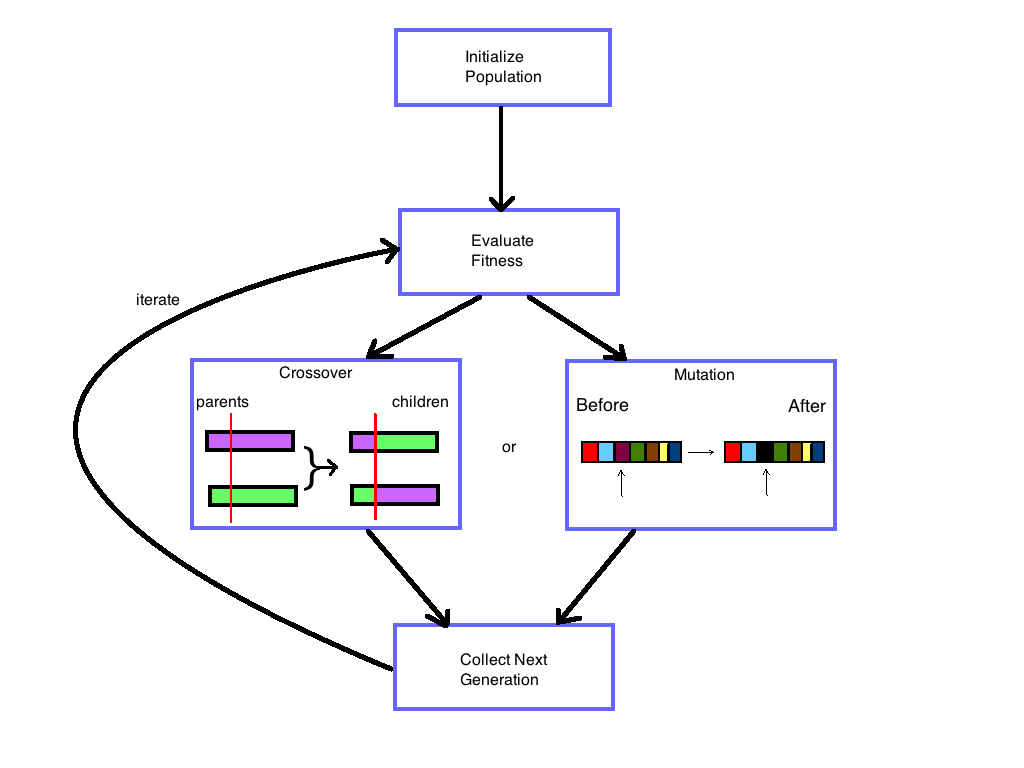
\includegraphics[scale=.34]{GA_exmaple.png}\\
	{\flushleft Example GA experiment:}\\
	$\begin{array}{cc}
		\fbox{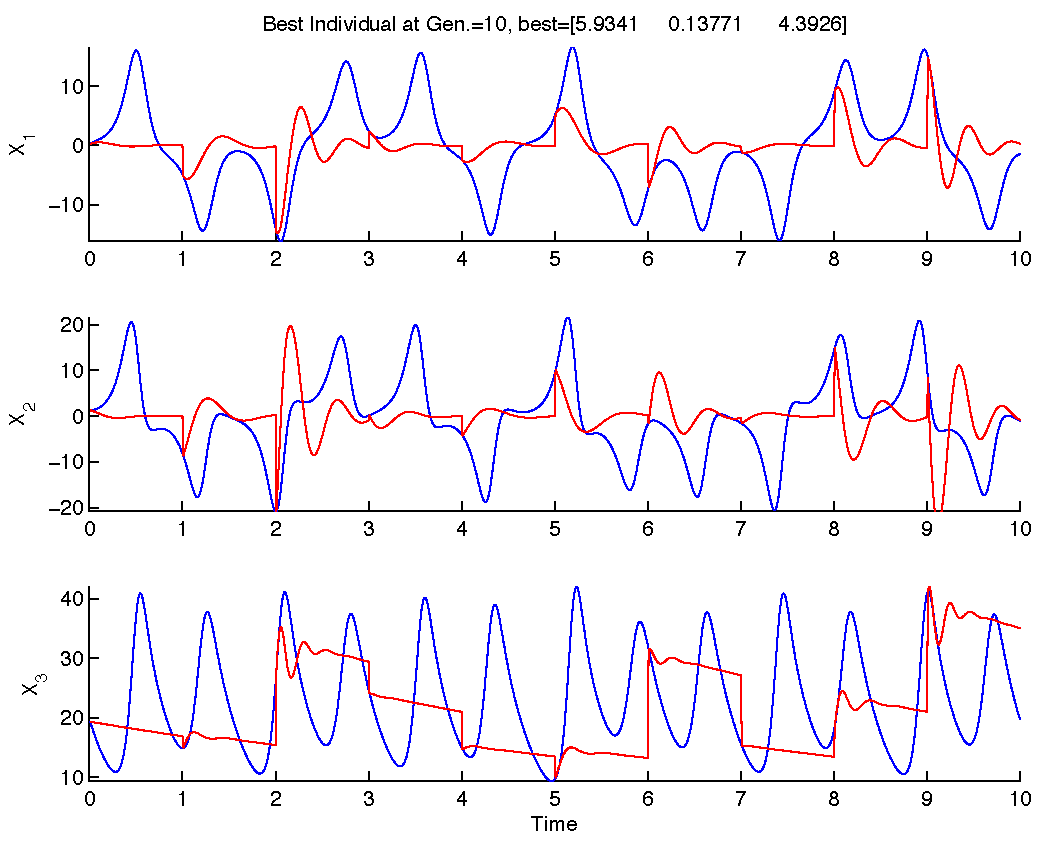
\includegraphics[width=.27\columnwidth]{sample.pdf}}&
		\hspace{-.3cm}\fbox{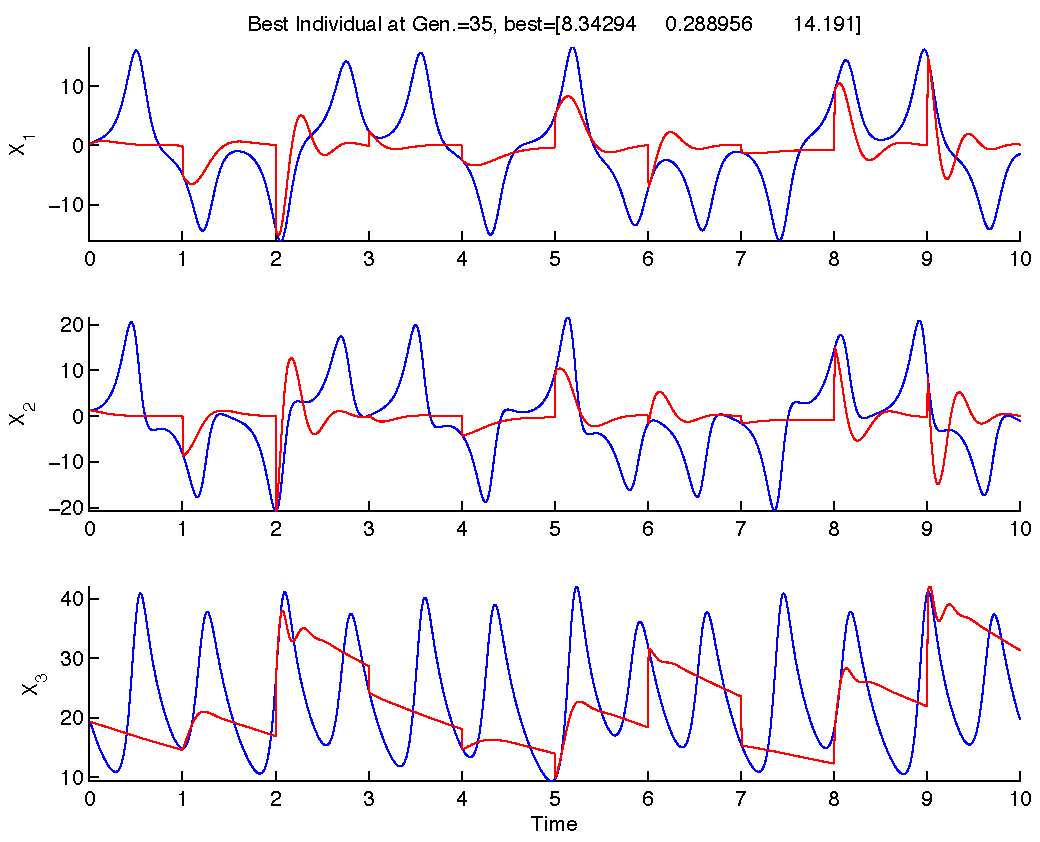
\includegraphics[width=.27\columnwidth]{sample2.pdf}}\\
		\fbox{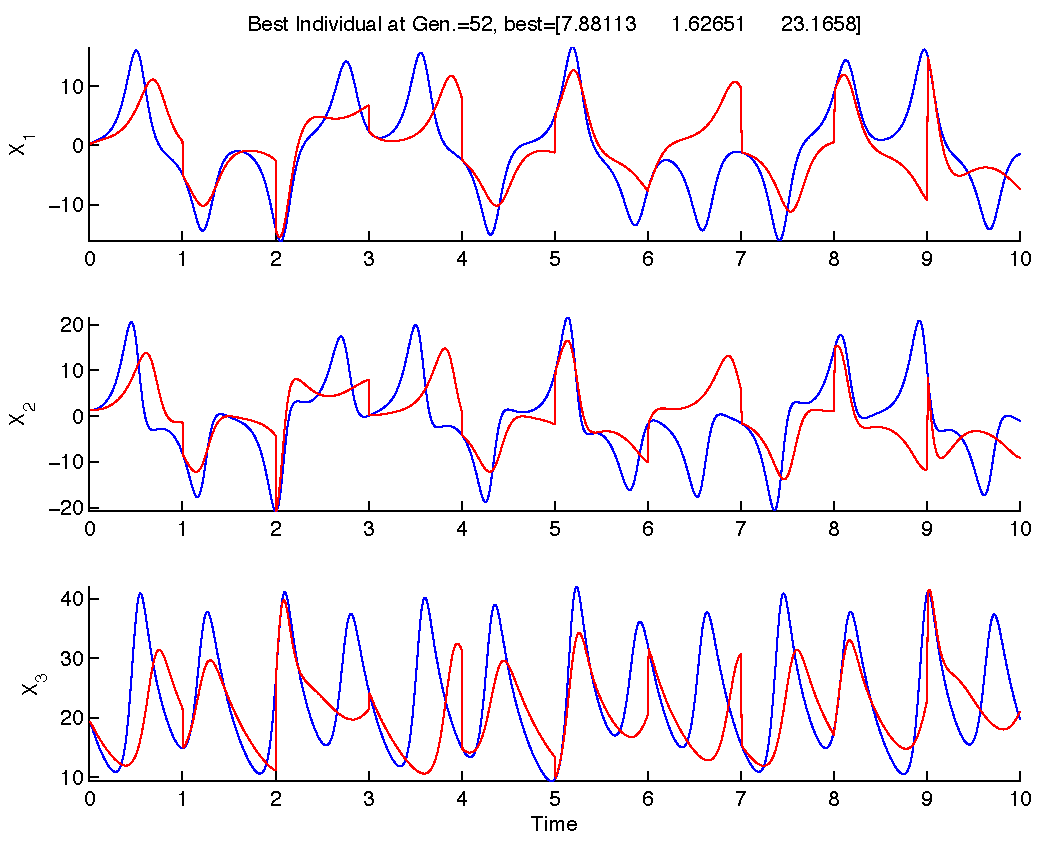
\includegraphics[width=.27\columnwidth]{sample3.pdf}}&		
		\hspace{-.3cm}\fbox{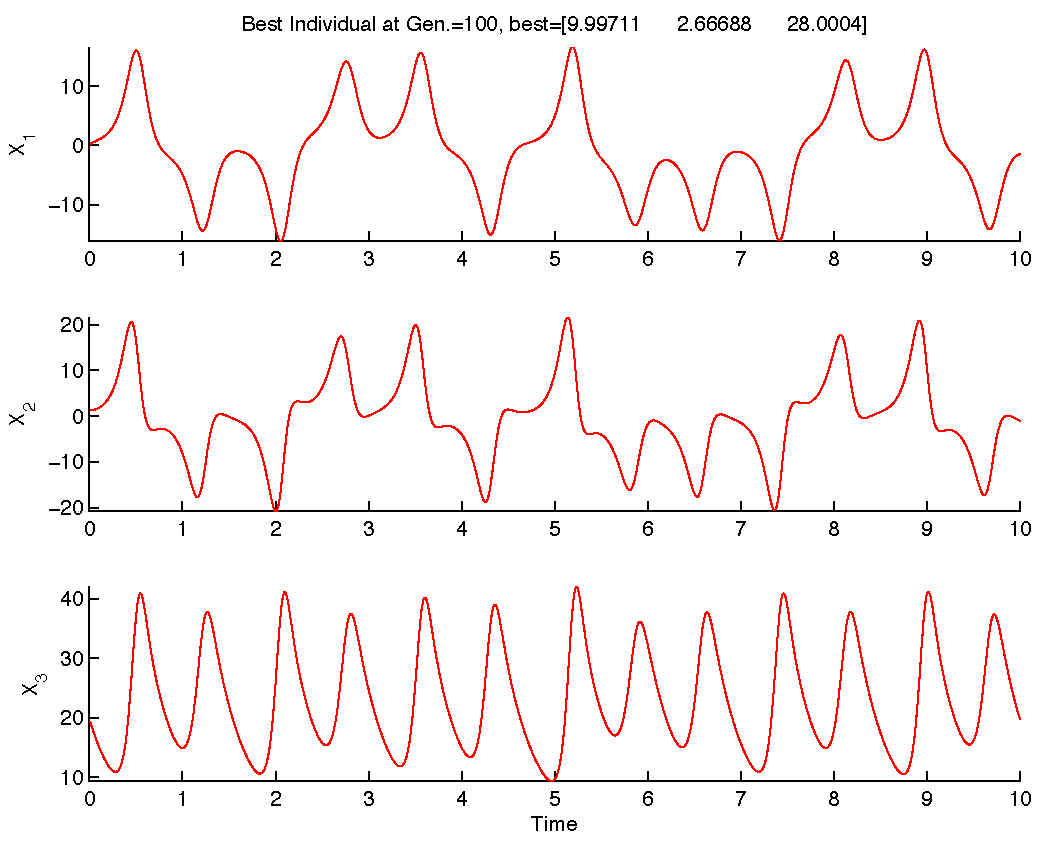
\includegraphics[width=.27\columnwidth]{sample4.pdf}}				
	\end{array}$
\end{center}
{\bf\small Figure 2. (Top) A cartoon demonstrating the flow of control for GA execution. The population of random real-valued vectors is initialized, and each individual has its fitness assessed. With some probability individuals are selected for single-point crossover or mutation. The children from these processes are collected into the new population. This process is iterated for a prescribed number of generations or until iteration fails to yield improvement. (Bottom) An example illustrating the improvement in parameter estimation made by the GA when attempting to recover the parameters ($\sigma=10,b=8/3,R=28$) over 100 generations. The observed data (truth) is in \textcolor{blue}{blue}, while the trajectory yielded from the best guess at the true parameters is provided in \textcolor{red}{red}. From left to right, we show the best solution after 10, 35, 52, and 100 generations. We see that at 100 generations, the best guess at the true parameters is reasonably close to the correct answer ($\sigma=9.99711,b=2.66688,R=28.0004$)}\\

\clearpage
\begin{center}
	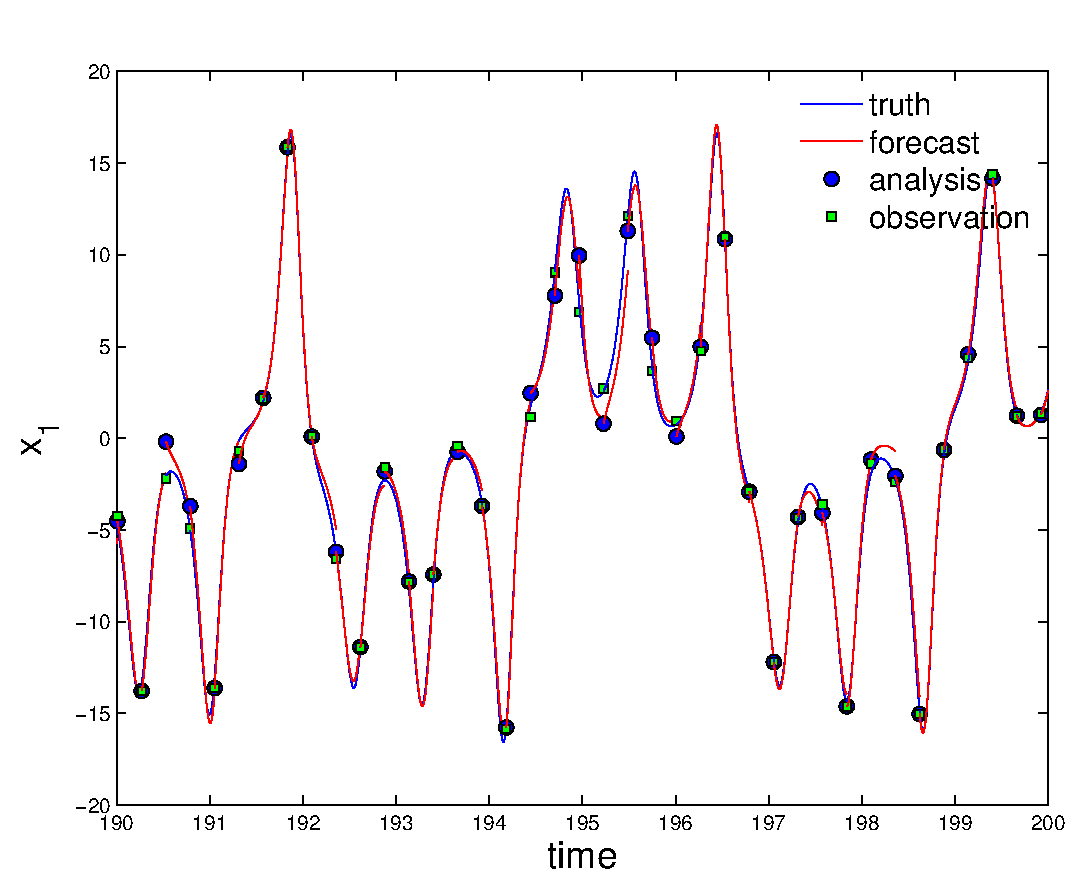
\includegraphics[scale=1.00]{DA-figure.pdf}\\
\end{center}
{\bf\small  Example DA experiment: showing the $x_1$ variable of the Lorenz 63 system, with a observation subsampling of 25. With observational error, the EKF predicts the data well, frequently making analyses that are closer to the truth than the observations.}\\
\clearpage

%%%%%%%%%%%%%%%%%%%%%%%%%%%%%%%%%%%%%%%%%%%%%%%%%%%%%%%%
\begin{thebibliography}{9}

        \bibitem{achtelik2009visual}
        Achtelik, M., T.~Zhang, K.~Kuhnlenz, and M.~Buss (2009).
        \newblock Visual tracking and control of a quadcopter using a stereo camera
          system and inertial sensors.
        \newblock In {\em Mechatronics and Automation, 2009. ICMA 2009. International
          Conference on}, pp.\	2863--2869. IEEE.
        
        \bibitem{siouris1997tracking}
        Siouris, G.~M., G.~Chen, and J.~Wang (1997).
        \newblock Tracking an incoming ballistic missile using an extended interval
          kalman filter.
        \newblock {\em Aerospace and Electronic Systems, IEEE Transactions on\/}~{\em
          33\/}(1), 232--240.
        
        \bibitem{talagrand1997assimilation}
        Talagrand, O. (1997).
        \newblock Assimilation of observations, an introduction.
        \newblock {\em JOURNAL-METEOROLOGICAL SOCIETY OF JAAN SERIES 2\/}~{\em 75},
          81--99.
        
        \bibitem{kalman1961new}
        Kalman, R. and R.~Bucy (1961).
        \newblock New results in linear prediction and filtering theory.
        \newblock {\em Trans. AMSE J. Basic Eng. D\/}~{\em 83}, 95--108.
        
        \bibitem{savely1972}
        Savely, R., B.~Cockrell, , and S.~Pines (1972).
        \newblock Apollo experience report - onboard navigational and alignment
          software.
        \newblock {\em Technical Report\/}.
        
        \bibitem{kalnay2003}
        Kalnay, E. (2003).
        \newblock {\em Atmospheric modeling, data assimilation, and predictability}.
        \newblock Cambridge university press.
        
        \bibitem{danforth2007estimating}
        Danforth, C.~M., E.~Kalnay, and T.~Miyoshi (2007).
        \newblock Estimating and correcting global weather model error.
        \newblock {\em Monthly weather review\/}~{\em 135\/}(2), 281--299.
        
        \bibitem{li2009accounting}
        Li, H., E.~Kalnay, T.~Miyoshi, and C.~M. Danforth (2009).
        \newblock Accounting for model errors in ensemble data assimilation.
        \newblock {\em Monthly Weather Review\/}~{\em 137\/}(10), 3407--3419.

        \bibitem{reagan2013}
        Reagan, A (2013).
        \newblock Predicting Flow Reversals in a Computational Fluid Dyanmics Simulated Thermosyphon Using Data Assimilatoin.
        \newblock University of Vermont Master's Thesis, {\em arXiv:1312.2142 [math.DS]}.

        \bibitem{kalnay20074}
        Kalnay, E., H.~Li, T.~Miyoshi, S.-C. YANG, and J.~BALLABRERA-POY (2007).
        \newblock 4-d-var or ensemble kalman filter?
        \newblock {\em Tellus A\/}~{\em 59\/}(5), 758--773.

        \bibitem{lorenz1963}
        Lorenz, E.~N. (1963).
        \newblock Deterministic nonperiodic flow.
        \newblock {\em Journal of the atmospheric sciences\/}~{\em 20\/}(2), 130--141.

        \bibitem{saltzman1962finite}
        Saltzman, B. (1962).
        \newblock Finite amplitude free convection as an initial value problem-i.
        \newblock {\em Journal of the Atmospheric Sciences\/}~{\em 19\/}(4), 329--341.

	\bibitem{kerr}
	R. A. Kerr. \emph{Weather Forecasts Slowly Clearing Up}. Science 9 November 2012: Vol. 338 no. 6108 pp. 734-737 DOI: 10.1126/science.338.6108.734

        \bibitem{farmer}
                Farmer, J. D., and J. J. Sidorowich. \emph{Predicting Chaotic Time Series.} Phys. Rev. Lett. 59(8) (1987): 845-848.

	\bibitem{orrell3}
	 D. Orrell, \emph{Role of the Metric in Forecast Error Growth: How Chaotic is
the Weather?}, Tellus 54A (2002) 350Ð362.
        \bibitem{D+Y}
        	C. M. Danforth, J. A. Yorke.  2006. \emph{Making Forecasts for Chaotic Physical Processes.}
		Physical Review Letters, 96, 144102.
 	\bibitem{lorenz95}
	E.N. Lorenz, \emph{Predictability A problem partly solved}, in: ECMWF Seminar Proceedings on Predictability, Reading, United
Kingdom, ECMWF, 1995, pp. 118.
         \bibitem{lorenz68}
                E. N. Lorenz. \emph{The predictability of a flow which possesses many scales of motion}. {\bf Tellus XXI}, 289 (1968).
	\bibitem{lorenz98}
	E.N. Lorenz, K.A. Emanuel, \emph{Optimal sites for supplementary weather observations: simulation with a small model}, J. Atmos. Sci.
55 (1998) 399Ð414.
         \bibitem{lorenzAttr}
                Lorenz, Edward N., 1963: \emph{Deterministic Nonperiodic Flow}. {\it J. Atmos. Sci.}, {\bf 20}, 130.141.
           \bibitem{lorenz96} 
                E. N. Lorenz, Proc. Seminar on Predictability 1, 1 (1996).
        \bibitem{england}
                R. England. \emph{Error estimates for Runga-Kutta type solutions to systems of ordinary differential equations}. {\it The Computer Journal} (1969) 12 (2): 166-170. doi: 10.1093/comjnl/12.2.166
%        \bibitem{werneth}
%                Charles M Werneth et al 2010 Eur. J. Phys. {\bf (31)} 693 doi:10.1088/0143-0807/31/3/027
        \bibitem{wilks}
         D. S. Wilks, \emph{Effects of Stochastic Parametrizations in the Lorenz Õ96 System}, Quart. J. Roy. Meteo. Soc. 131 (2005) 389Ð407.

	\bibitem{GA1}
		J. Horn, N. Nafpliotis, and D.E. Goldberg. \emph{A niched Pareto genetic algorithm for multiobjective optimization}. Evolutionary Computation, 1994. IEEE World Congress on Computational Intelligence., Proceedings of the First IEEE Conference on (1994) 1: 82-87. doi:10.1109/ICEC.1994.350037
%@INPROCEEDINGS{GA1, 
%author={Horn, J. and Nafpliotis, N. and Goldberg, D.E.}, 
%booktitle={Evolutionary Computation, 1994. IEEE World Congress on Computational Intelligence., Proceedings of the First IEEE Conference on}, 
%title={A niched Pareto genetic algorithm for multiobjective optimization}, 
%year={1994}, 
%pages={82-87 vol.1}, 
%keywords={genetic algorithms;operations research;optimisation;Niched Pareto GA;Pareto genetic algorithm;Pareto optimal set;genetic algorithm;multiobjective optimization;multiple objectives;niching pressure;optimization problems;Bioinformatics;Contracts;Costs;Genetic algorithms;Genomics;Internet;NASA;Pareto optimization;Sampling methods;Turning}, 
%doi={10.1109/ICEC.1994.350037}}
	\bibitem{GA2}
		K. Deb, A. Pratap, S. Agarwal, and T. Meyarivan. \emph{A fast and elitist multiobjective genetic algorithm: NSGA-II}. Evolutionary Computation, IEEE Transactions on 6 (2): 182-197. doi:10.1109/4235.996017
%@ARTICLE{GA1, 
%author={Deb, K. and Pratap, A. and Agarwal, S. and Meyarivan, T.}, 
%journal={Evolutionary Computation, IEEE Transactions on}, 
%title={A fast and elitist multiobjective genetic algorithm: NSGA-II}, 
%year={2002}, 
%volume={6}, 
%number={2}, 
%pages={182-197}, 
%keywords={Pareto distribution;computational complexity;constraint theory;convergence;genetic algorithms;operations research;simulation;sorting;NSGA-II;Nondominated Sorting Genetic Algorithm II;Pareto-archived evolution strategy;Pareto-optimal front;algorithm performance;computational complexity;constrained multi-objective problems;constraint handling;convergence;dominance definition;fast elitist multi-objective genetic algorithm;mating pool;multi-criterion decision making;multi-objective evolutionary algorithm;multi-objective optimization;nondominated sharing;nonlinear problem;objectives;parent/offspring population combination;population size;selection operator;simulation;solution fitness;solution spread;strength-Pareto evolutionary algorithm;Associate members;Computational complexity;Computational modeling;Constraint optimization;Decision making;Diversity reception;Evolutionary computation;Genetic algorithms;Sorting;Testing}, 
%doi={10.1109/4235.996017}, 
%ISSN={1089-778X}}

	\bibitem{Shin2002321}
		K-S Shin, Y-J Lee. \emph{A genetic algorithm application in bankruptcy prediction modeling}. Expert Systems w/ Applications (2002) 23 (3): 321-328. doi = "http://dx.doi.org/10.1016/S0957-4174(02)00051-9"
%@article{Shin2002321,
%title = "A genetic algorithm application in bankruptcy prediction modeling ",
%journal = "Expert Systems with Applications ",
%volume = "23",
%number = "3",
%pages = "321 - 328",
%year = "2002",
%note = "",
%issn = "0957-4174",
%doi = "http://dx.doi.org/10.1016/S0957-4174(02)00051-9",
%url = "http://www.sciencedirect.com/science/article/pii/S0957417402000519",
%author = "Kyung-Shik Shin and Yong-Joo Lee",
%keywords = "Genetic algorithms",
%keywords = "Rule extraction",
%keywords = "Bankruptcy prediction "
%}
	\bibitem{WRR}
		Q. J. Wang. \emph{The Genetic Algorithm and its Application to Calibrating Conceptual Rainfall-Runoff Models}. Water Resources Research 27 (9): 2467-2471. dpi:http://dx.doi.org/10.1029/91WR01305
%@article {WRR,
%author = {Wang, Q. J.},
%title = {The Genetic Algorithm and Its Application to Calibrating Conceptual Rainfall-Runoff Models},
%journal = {Water Resources Research},
%volume = {27},
%number = {9},
%issn = {1944-7973},
%url = {http://dx.doi.org/10.1029/91WR01305},
%doi = {10.1029/91WR01305},
%pages = {2467--2471},
%year = {1991},
%}

\bibitem{CEM}
R. Leardi. \emph{Application of genetic algorithm-PLS for feature selection in spectral data sets}. Journal of Chemometrics 14 (5-6): 643-655: DOI: 10.1002/1099-128X(200009/12)14:5/6<643::AID-CEM621>3.0.CO;2-E
%@article {CEM,
%author = {Leardi, Riccardo},
%title = {Application of genetic algorithm窶撤LS for feature selection in spectral data sets},
%journal = {Journal of Chemometrics},
%volume = {14},
%number = {5-6},
%publisher = {John Wiley & Sons, Ltd.},
%issn = {1099-128X},
%url = {http://dx.doi.org/10.1002/1099-128X(200009/12)14:5/6<643::AID-CEM621>3.0.CO;2-E},
%doi = {10.1002/1099-128X(200009/12)14:5/6<643::AID-CEM621>3.0.CO;2-E},
%pages = {643--655},
%keywords = {genetic algorithms, feature selection, PLS regression, spectral data},
%year = {2000},
%}

\end{thebibliography}
\end{multicols}

\section{Appendix}
\subsection{Experimental Results}

\input{tableOutput.txt}

\begin{multicols}{3} 
\tiny 

\subsubsection{Lorenz '63 (all Variables)}
Parameters: $\sigma=10, b=8/3, R=22$\\
noise Type: normal with magnitude 0, using every 1 observation(s) of first 1 variables.\\
\begin{tabular}{cccc}
\hline Experiment ID & b & $\sigma$ & R \\ \hline 
0 & nan & nan & nan\\ \hline 
 1 & nan & nan & nan\\ \hline 
 2 & nan & nan & nan\\ \hline 
 3 & nan & nan & nan\\ \hline 
 4 & nan & nan & nan\\ \hline 
 \end{tabular}\\
Parameters: $\sigma=10, b=8/3, R=22$\\
noise Type: normal with magnitude 0, using every 5 observation(s) of first 1 variables.\\
\begin{tabular}{cccc}
\hline Experiment ID & b & $\sigma$ & R \\ \hline 
0 & nan & nan & nan\\ \hline 
 1 & nan & nan & nan\\ \hline 
 2 & nan & nan & nan\\ \hline 
 3 & nan & nan & nan\\ \hline 
 4 & nan & nan & nan\\ \hline 
 \end{tabular}\\
Parameters: $\sigma=10, b=8/3, R=22$\\
noise Type: normal with magnitude 0, using every 25 observation(s) of first 1 variables.\\
\begin{tabular}{cccc}
\hline Experiment ID & b & $\sigma$ & R \\ \hline 
0 & nan & nan & nan\\ \hline 
 1 & nan & nan & nan\\ \hline 
 2 & nan & nan & nan\\ \hline 
 3 & nan & nan & nan\\ \hline 
 4 & nan & nan & nan\\ \hline 
 \end{tabular}\\
Parameters: $\sigma=10, b=8/3, R=22$\\
noise Type: normal with magnitude 0, using every 50 observation(s) of first 1 variables.\\
\begin{tabular}{cccc}
\hline Experiment ID & b & $\sigma$ & R \\ \hline 
0 & nan & nan & nan\\ \hline 
 1 & nan & nan & nan\\ \hline 
 2 & nan & nan & nan\\ \hline 
 3 & nan & nan & nan\\ \hline 
 4 & nan & nan & nan\\ \hline 
 \end{tabular}\\
Parameters: $\sigma=10, b=8/3, R=22$\\
noise Type: normal with magnitude 0.01, using every 1 observation(s) of first 1 variables.\\
\begin{tabular}{cccc}
\hline Experiment ID & b & $\sigma$ & R \\ \hline 
0 & 2.6513 & 9.9041 & 22.089\\ \hline 
 1 & 2.6513 & 9.9041 & 22.089\\ \hline 
 2 & 2.6513 & 9.9041 & 22.089\\ \hline 
 3 & 2.6513 & 9.9041 & 22.089\\ \hline 
 4 & 2.6513 & 9.9041 & 22.089\\ \hline 
 \end{tabular}\\
Parameters: $\sigma=10, b=8/3, R=22$\\
noise Type: normal with magnitude 0.01, using every 5 observation(s) of first 1 variables.\\
\begin{tabular}{cccc}
\hline Experiment ID & b & $\sigma$ & R \\ \hline 
0 & 2.6641 & 9.9993 & 22.02\\ \hline 
 1 & 2.6641 & 9.9993 & 22.02\\ \hline 
 2 & 2.6641 & 9.9993 & 22.02\\ \hline 
 3 & 2.6641 & 9.9993 & 22.02\\ \hline 
 4 & 2.6641 & 9.9993 & 22.02\\ \hline 
 \end{tabular}\\
Parameters: $\sigma=10, b=8/3, R=22$\\
noise Type: normal with magnitude 0.01, using every 25 observation(s) of first 1 variables.\\
\begin{tabular}{cccc}
\hline Experiment ID & b & $\sigma$ & R \\ \hline 
0 & nan & nan & nan\\ \hline 
 1 & nan & nan & nan\\ \hline 
 2 & nan & nan & nan\\ \hline 
 3 & nan & nan & nan\\ \hline 
 4 & nan & nan & nan\\ \hline 
 \end{tabular}\\
Parameters: $\sigma=10, b=8/3, R=22$\\
noise Type: normal with magnitude 0.01, using every 50 observation(s) of first 1 variables.\\
\begin{tabular}{cccc}
\hline Experiment ID & b & $\sigma$ & R \\ \hline 
0 & nan & nan & nan\\ \hline 
 1 & nan & nan & nan\\ \hline 
 2 & nan & nan & nan\\ \hline 
 3 & nan & nan & nan\\ \hline 
 4 & nan & nan & nan\\ \hline 
 \end{tabular}\\
Parameters: $\sigma=10, b=8/3, R=22$\\
noise Type: normal with magnitude 0.05, using every 1 observation(s) of first 1 variables.\\
\begin{tabular}{cccc}
\hline Experiment ID & b & $\sigma$ & R \\ \hline 
0 & 2.692 & 9.9964 & 21.786\\ \hline 
 1 & 2.692 & 9.9964 & 21.786\\ \hline 
 2 & 2.692 & 9.9964 & 21.786\\ \hline 
 3 & 2.692 & 9.9964 & 21.786\\ \hline 
 4 & 2.692 & 9.9964 & 21.786\\ \hline 
 \end{tabular}\\
Parameters: $\sigma=10, b=8/3, R=22$\\
noise Type: normal with magnitude 0.05, using every 5 observation(s) of first 1 variables.\\
\begin{tabular}{cccc}
\hline Experiment ID & b & $\sigma$ & R \\ \hline 
0 & 2.6579 & 9.9885 & 22.07\\ \hline 
 1 & 2.6579 & 9.9885 & 22.07\\ \hline 
 2 & 2.6579 & 9.9885 & 22.07\\ \hline 
 3 & 2.6579 & 9.9885 & 22.07\\ \hline 
 4 & 2.6579 & 9.9885 & 22.07\\ \hline 
 \end{tabular}\\
Parameters: $\sigma=10, b=8/3, R=22$\\
noise Type: normal with magnitude 0.05, using every 25 observation(s) of first 1 variables.\\
\begin{tabular}{cccc}
\hline Experiment ID & b & $\sigma$ & R \\ \hline 
0 & nan & nan & nan\\ \hline 
 1 & nan & nan & nan\\ \hline 
 2 & nan & nan & nan\\ \hline 
 3 & nan & nan & nan\\ \hline 
 4 & nan & nan & nan\\ \hline 
 \end{tabular}\\
Parameters: $\sigma=10, b=8/3, R=22$\\
noise Type: normal with magnitude 0.05, using every 50 observation(s) of first 1 variables.\\
\begin{tabular}{cccc}
\hline Experiment ID & b & $\sigma$ & R \\ \hline 
0 & nan & nan & nan\\ \hline 
 1 & nan & nan & nan\\ \hline 
 2 & nan & nan & nan\\ \hline 
 3 & nan & nan & nan\\ \hline 
 4 & nan & nan & nan\\ \hline 
 \end{tabular}\\
Parameters: $\sigma=10, b=8/3, R=22$\\
noise Type: normal with magnitude 0.1, using every 1 observation(s) of first 1 variables.\\
\begin{tabular}{cccc}
\hline Experiment ID & b & $\sigma$ & R \\ \hline 
0 & 2.6857 & 9.9685 & 21.833\\ \hline 
 1 & 2.6857 & 9.9685 & 21.833\\ \hline 
 2 & 2.6857 & 9.9685 & 21.833\\ \hline 
 3 & 2.6857 & 9.9685 & 21.833\\ \hline 
 4 & 2.6857 & 9.9685 & 21.833\\ \hline 
 \end{tabular}\\
Parameters: $\sigma=10, b=8/3, R=22$\\
noise Type: normal with magnitude 0.1, using every 5 observation(s) of first 1 variables.\\
\begin{tabular}{cccc}
\hline Experiment ID & b & $\sigma$ & R \\ \hline 
0 & 2.6575 & 9.9249 & 22.076\\ \hline 
 1 & 2.6575 & 9.9249 & 22.076\\ \hline 
 2 & 2.6575 & 9.9249 & 22.076\\ \hline 
 3 & 2.6575 & 9.9249 & 22.076\\ \hline 
 4 & 2.6575 & 9.9249 & 22.076\\ \hline 
 \end{tabular}\\
Parameters: $\sigma=10, b=8/3, R=22$\\
noise Type: normal with magnitude 0.1, using every 25 observation(s) of first 1 variables.\\
\begin{tabular}{cccc}
\hline Experiment ID & b & $\sigma$ & R \\ \hline 
0 & nan & nan & nan\\ \hline 
 1 & nan & nan & nan\\ \hline 
 2 & nan & nan & nan\\ \hline 
 3 & nan & nan & nan\\ \hline 
 4 & nan & nan & nan\\ \hline 
 \end{tabular}\\
Parameters: $\sigma=10, b=8/3, R=22$\\
noise Type: normal with magnitude 0.1, using every 50 observation(s) of first 1 variables.\\
\begin{tabular}{cccc}
\hline Experiment ID & b & $\sigma$ & R \\ \hline 
0 & nan & nan & nan\\ \hline 
 1 & nan & nan & nan\\ \hline 
 2 & nan & nan & nan\\ \hline 
 3 & nan & nan & nan\\ \hline 
 4 & nan & nan & nan\\ \hline 
 \end{tabular}\\
Parameters: $\sigma=10, b=8/3, R=22$\\
noise Type: normal with magnitude 0.25, using every 1 observation(s) of first 1 variables.\\
\begin{tabular}{cccc}
\hline Experiment ID & b & $\sigma$ & R \\ \hline 
0 & 2.7263 & 9.6664 & 21.488\\ \hline 
 1 & 2.7263 & 9.6664 & 21.488\\ \hline 
 2 & 2.7263 & 9.6664 & 21.488\\ \hline 
 3 & 2.7263 & 9.6664 & 21.488\\ \hline 
 4 & 2.7263 & 9.6664 & 21.488\\ \hline 
 \end{tabular}\\
Parameters: $\sigma=10, b=8/3, R=22$\\
noise Type: normal with magnitude 0.25, using every 5 observation(s) of first 1 variables.\\
\begin{tabular}{cccc}
\hline Experiment ID & b & $\sigma$ & R \\ \hline 
0 & 2.6715 & 9.8862 & 21.977\\ \hline 
 1 & 2.6715 & 9.8862 & 21.977\\ \hline 
 2 & 2.6715 & 9.8862 & 21.977\\ \hline 
 3 & 2.6715 & 9.8862 & 21.977\\ \hline 
 4 & 2.6715 & 9.8862 & 21.977\\ \hline 
 \end{tabular}\\
Parameters: $\sigma=10, b=8/3, R=22$\\
noise Type: normal with magnitude 0.25, using every 25 observation(s) of first 1 variables.\\
\begin{tabular}{cccc}
\hline Experiment ID & b & $\sigma$ & R \\ \hline 
0 & nan & nan & nan\\ \hline 
 1 & nan & nan & nan\\ \hline 
 2 & nan & nan & nan\\ \hline 
 3 & nan & nan & nan\\ \hline 
 4 & nan & nan & nan\\ \hline 
 \end{tabular}\\
Parameters: $\sigma=10, b=8/3, R=22$\\
noise Type: normal with magnitude 0.25, using every 50 observation(s) of first 1 variables.\\
\begin{tabular}{cccc}
\hline Experiment ID & b & $\sigma$ & R \\ \hline 
0 & 4.2404 & 33.763 & -7.259\\ \hline 
 1 & 4.2404 & 33.763 & -7.259\\ \hline 
 2 & 4.2404 & 33.763 & -7.259\\ \hline 
 3 & 4.2404 & 33.763 & -7.259\\ \hline 
 4 & 4.2404 & 33.763 & -7.259\\ \hline 
 \end{tabular}\\
Parameters: $\sigma=10, b=8/3, R=22$\\
noise Type: normal with magnitude 0.5, using every 1 observation(s) of first 1 variables.\\
\begin{tabular}{cccc}
\hline Experiment ID & b & $\sigma$ & R \\ \hline 
0 & 2.7172 & 9.6206 & 21.437\\ \hline 
 1 & 2.7172 & 9.6206 & 21.437\\ \hline 
 2 & 2.7172 & 9.6206 & 21.437\\ \hline 
 3 & 2.7172 & 9.6206 & 21.437\\ \hline 
 4 & 2.7172 & 9.6206 & 21.437\\ \hline 
 \end{tabular}\\
Parameters: $\sigma=10, b=8/3, R=22$\\
noise Type: normal with magnitude 0.5, using every 5 observation(s) of first 1 variables.\\
\begin{tabular}{cccc}
\hline Experiment ID & b & $\sigma$ & R \\ \hline 
0 & 2.6821 & 9.8642 & 21.904\\ \hline 
 1 & 2.6821 & 9.8642 & 21.904\\ \hline 
 2 & 2.6821 & 9.8642 & 21.904\\ \hline 
 3 & 2.6821 & 9.8642 & 21.904\\ \hline 
 4 & 2.6821 & 9.8642 & 21.904\\ \hline 
 \end{tabular}\\
Parameters: $\sigma=10, b=8/3, R=22$\\
noise Type: normal with magnitude 0.5, using every 25 observation(s) of first 1 variables.\\
\begin{tabular}{cccc}
\hline Experiment ID & b & $\sigma$ & R \\ \hline 
0 & nan & nan & nan\\ \hline 
 1 & nan & nan & nan\\ \hline 
 2 & nan & nan & nan\\ \hline 
 3 & nan & nan & nan\\ \hline 
 4 & nan & nan & nan\\ \hline 
 \end{tabular}\\
Parameters: $\sigma=10, b=8/3, R=22$\\
noise Type: normal with magnitude 0.5, using every 50 observation(s) of first 1 variables.\\
\begin{tabular}{cccc}
\hline Experiment ID & b & $\sigma$ & R \\ \hline 
0 & 5.2708 & -0.21294 & 11.562\\ \hline 
 1 & 5.2708 & -0.21294 & 11.562\\ \hline 
 2 & 5.2708 & -0.21294 & 11.562\\ \hline 
 3 & 5.2708 & -0.21294 & 11.562\\ \hline 
 4 & 5.2708 & -0.21294 & 11.562\\ \hline 
 \end{tabular}\\
Parameters: $\sigma=10, b=8/3, R=22$\\
noise Type: normal with magnitude 1, using every 1 observation(s) of first 1 variables.\\
\begin{tabular}{cccc}
\hline Experiment ID & b & $\sigma$ & R \\ \hline 
0 & 2.7143 & 9.5407 & 21.386\\ \hline 
 1 & 2.7143 & 9.5407 & 21.386\\ \hline 
 2 & 2.7143 & 9.5407 & 21.386\\ \hline 
 3 & 2.7143 & 9.5407 & 21.386\\ \hline 
 4 & 2.7143 & 9.5407 & 21.386\\ \hline 
 \end{tabular}\\
Parameters: $\sigma=10, b=8/3, R=22$\\
noise Type: normal with magnitude 1, using every 5 observation(s) of first 1 variables.\\
\begin{tabular}{cccc}
\hline Experiment ID & b & $\sigma$ & R \\ \hline 
0 & 3.0825 & 10.171 & 19.214\\ \hline 
 1 & 3.0825 & 10.171 & 19.214\\ \hline 
 2 & 3.0825 & 10.171 & 19.214\\ \hline 
 3 & 3.0825 & 10.171 & 19.214\\ \hline 
 4 & 3.0825 & 10.171 & 19.214\\ \hline 
 \end{tabular}\\
Parameters: $\sigma=10, b=8/3, R=22$\\
noise Type: normal with magnitude 1, using every 25 observation(s) of first 1 variables.\\
\begin{tabular}{cccc}
\hline Experiment ID & b & $\sigma$ & R \\ \hline 
0 & nan & nan & nan\\ \hline 
 1 & nan & nan & nan\\ \hline 
 2 & nan & nan & nan\\ \hline 
 3 & nan & nan & nan\\ \hline 
 4 & nan & nan & nan\\ \hline 
 \end{tabular}\\
Parameters: $\sigma=10, b=8/3, R=22$\\
noise Type: normal with magnitude 1, using every 50 observation(s) of first 1 variables.\\
\begin{tabular}{cccc}
\hline Experiment ID & b & $\sigma$ & R \\ \hline 
0 & 3.9608 & 2.3971 & 14.915\\ \hline 
 1 & 3.9608 & 2.3971 & 14.915\\ \hline 
 2 & 3.9608 & 2.3971 & 14.915\\ \hline 
 3 & 3.9608 & 2.3971 & 14.915\\ \hline 
 4 & 3.9608 & 2.3971 & 14.915\\ \hline 
 \end{tabular}\\
Parameters: $\sigma=10, b=8/3, R=22$\\
noise Type: normal with magnitude 2, using every 1 observation(s) of first 1 variables.\\
\begin{tabular}{cccc}
\hline Experiment ID & b & $\sigma$ & R \\ \hline 
0 & 2.7045 & 9.289 & 21.371\\ \hline 
 1 & 2.7045 & 9.289 & 21.371\\ \hline 
 2 & 2.7045 & 9.289 & 21.371\\ \hline 
 3 & 2.7045 & 9.289 & 21.371\\ \hline 
 4 & 2.7045 & 9.289 & 21.371\\ \hline 
 \end{tabular}\\
Parameters: $\sigma=10, b=8/3, R=22$\\
noise Type: normal with magnitude 2, using every 5 observation(s) of first 1 variables.\\
\begin{tabular}{cccc}
\hline Experiment ID & b & $\sigma$ & R \\ \hline 
0 & 3.7514 & 9.8205 & 16.029\\ \hline 
 1 & 3.7514 & 9.8205 & 16.029\\ \hline 
 2 & 3.7514 & 9.8205 & 16.029\\ \hline 
 3 & 3.7514 & 9.8205 & 16.029\\ \hline 
 4 & 3.7514 & 9.8205 & 16.029\\ \hline 
 \end{tabular}\\
Parameters: $\sigma=10, b=8/3, R=22$\\
noise Type: normal with magnitude 2, using every 25 observation(s) of first 1 variables.\\
\begin{tabular}{cccc}
\hline Experiment ID & b & $\sigma$ & R \\ \hline 
0 & nan & nan & nan\\ \hline 
 1 & nan & nan & nan\\ \hline 
 2 & nan & nan & nan\\ \hline 
 3 & nan & nan & nan\\ \hline 
 4 & nan & nan & nan\\ \hline 
 \end{tabular}\\
Parameters: $\sigma=10, b=8/3, R=22$\\
noise Type: normal with magnitude 2, using every 50 observation(s) of first 1 variables.\\
\begin{tabular}{cccc}
\hline Experiment ID & b & $\sigma$ & R \\ \hline 
0 & 3.7842 & 2.6283 & 15.308\\ \hline 
 1 & 3.7842 & 2.6283 & 15.308\\ \hline 
 2 & 3.7842 & 2.6283 & 15.308\\ \hline 
 3 & 3.7842 & 2.6283 & 15.308\\ \hline 
 4 & 3.7842 & 2.6283 & 15.308\\ \hline 
 \end{tabular}\\
Parameters: $\sigma=10, b=8/3, R=22$\\
noise Type: normal with magnitude 0, using every 1 observation(s) of first 3 variables.\\
\begin{tabular}{cccc}
\hline Experiment ID & b & $\sigma$ & R \\ \hline 
0 & nan & nan & nan\\ \hline 
 1 & nan & nan & nan\\ \hline 
 2 & nan & nan & nan\\ \hline 
 3 & nan & nan & nan\\ \hline 
 4 & nan & nan & nan\\ \hline 
 \end{tabular}\\
Parameters: $\sigma=10, b=8/3, R=22$\\
noise Type: normal with magnitude 0, using every 5 observation(s) of first 3 variables.\\
\begin{tabular}{cccc}
\hline Experiment ID & b & $\sigma$ & R \\ \hline 
0 & nan & nan & nan\\ \hline 
 1 & nan & nan & nan\\ \hline 
 2 & nan & nan & nan\\ \hline 
 3 & nan & nan & nan\\ \hline 
 4 & nan & nan & nan\\ \hline 
 \end{tabular}\\
Parameters: $\sigma=10, b=8/3, R=22$\\
noise Type: normal with magnitude 0, using every 25 observation(s) of first 3 variables.\\
\begin{tabular}{cccc}
\hline Experiment ID & b & $\sigma$ & R \\ \hline 
0 & nan & nan & nan\\ \hline 
 1 & nan & nan & nan\\ \hline 
 2 & nan & nan & nan\\ \hline 
 3 & nan & nan & nan\\ \hline 
 4 & nan & nan & nan\\ \hline 
 \end{tabular}\\
Parameters: $\sigma=10, b=8/3, R=22$\\
noise Type: normal with magnitude 0, using every 50 observation(s) of first 3 variables.\\
\begin{tabular}{cccc}
\hline Experiment ID & b & $\sigma$ & R \\ \hline 
0 & nan & nan & nan\\ \hline 
 1 & nan & nan & nan\\ \hline 
 2 & nan & nan & nan\\ \hline 
 3 & nan & nan & nan\\ \hline 
 4 & nan & nan & nan\\ \hline 
 \end{tabular}\\
Parameters: $\sigma=10, b=8/3, R=22$\\
noise Type: normal with magnitude 0.01, using every 1 observation(s) of first 3 variables.\\
\begin{tabular}{cccc}
\hline Experiment ID & b & $\sigma$ & R \\ \hline 
0 & 2.6666 & 10.0 & 22.0\\ \hline 
 1 & 2.6666 & 10.0 & 22.0\\ \hline 
 2 & 2.6666 & 10.0 & 22.0\\ \hline 
 3 & 2.6666 & 10.0 & 22.0\\ \hline 
 4 & 2.6666 & 10.0 & 22.0\\ \hline 
 \end{tabular}\\
Parameters: $\sigma=10, b=8/3, R=22$\\
noise Type: normal with magnitude 0.01, using every 5 observation(s) of first 3 variables.\\
\begin{tabular}{cccc}
\hline Experiment ID & b & $\sigma$ & R \\ \hline 
0 & nan & nan & nan\\ \hline 
 1 & nan & nan & nan\\ \hline 
 2 & nan & nan & nan\\ \hline 
 3 & nan & nan & nan\\ \hline 
 4 & nan & nan & nan\\ \hline 
 \end{tabular}\\
Parameters: $\sigma=10, b=8/3, R=22$\\
noise Type: normal with magnitude 0.01, using every 25 observation(s) of first 3 variables.\\
\begin{tabular}{cccc}
\hline Experiment ID & b & $\sigma$ & R \\ \hline 
0 & nan & nan & nan\\ \hline 
 1 & nan & nan & nan\\ \hline 
 2 & nan & nan & nan\\ \hline 
 3 & nan & nan & nan\\ \hline 
 4 & nan & nan & nan\\ \hline 
 \end{tabular}\\
Parameters: $\sigma=10, b=8/3, R=22$\\
noise Type: normal with magnitude 0.01, using every 50 observation(s) of first 3 variables.\\
\begin{tabular}{cccc}
\hline Experiment ID & b & $\sigma$ & R \\ \hline 
0 & 2.6027 & -0.34153 & 21.996\\ \hline 
 1 & 2.6027 & -0.34153 & 21.996\\ \hline 
 2 & 2.6027 & -0.34153 & 21.996\\ \hline 
 3 & 2.6027 & -0.34153 & 21.996\\ \hline 
 4 & 2.6027 & -0.34153 & 21.996\\ \hline 
 \end{tabular}\\
Parameters: $\sigma=10, b=8/3, R=22$\\
noise Type: normal with magnitude 0.05, using every 1 observation(s) of first 3 variables.\\
\begin{tabular}{cccc}
\hline Experiment ID & b & $\sigma$ & R \\ \hline 
0 & 2.6663 & 10.0 & 22.0\\ \hline 
 1 & 2.6663 & 10.0 & 22.0\\ \hline 
 2 & 2.6663 & 10.0 & 22.0\\ \hline 
 3 & 2.6663 & 10.0 & 22.0\\ \hline 
 4 & 2.6663 & 10.0 & 22.0\\ \hline 
 \end{tabular}\\
Parameters: $\sigma=10, b=8/3, R=22$\\
noise Type: normal with magnitude 0.05, using every 5 observation(s) of first 3 variables.\\
\begin{tabular}{cccc}
\hline Experiment ID & b & $\sigma$ & R \\ \hline 
0 & nan & nan & nan\\ \hline 
 1 & nan & nan & nan\\ \hline 
 2 & nan & nan & nan\\ \hline 
 3 & nan & nan & nan\\ \hline 
 4 & nan & nan & nan\\ \hline 
 \end{tabular}\\
Parameters: $\sigma=10, b=8/3, R=22$\\
noise Type: normal with magnitude 0.05, using every 25 observation(s) of first 3 variables.\\
\begin{tabular}{cccc}
\hline Experiment ID & b & $\sigma$ & R \\ \hline 
0 & nan & nan & nan\\ \hline 
 1 & nan & nan & nan\\ \hline 
 2 & nan & nan & nan\\ \hline 
 3 & nan & nan & nan\\ \hline 
 4 & nan & nan & nan\\ \hline 
 \end{tabular}\\
Parameters: $\sigma=10, b=8/3, R=22$\\
noise Type: normal with magnitude 0.05, using every 50 observation(s) of first 3 variables.\\
\begin{tabular}{cccc}
\hline Experiment ID & b & $\sigma$ & R \\ \hline 
0 & 2.5516 & 10.217 & 22.012\\ \hline 
 1 & 2.5516 & 10.217 & 22.012\\ \hline 
 2 & 2.5516 & 10.217 & 22.012\\ \hline 
 3 & 2.5516 & 10.217 & 22.012\\ \hline 
 4 & 2.5516 & 10.217 & 22.012\\ \hline 
 \end{tabular}\\
Parameters: $\sigma=10, b=8/3, R=22$\\
noise Type: normal with magnitude 0.1, using every 1 observation(s) of first 3 variables.\\
\begin{tabular}{cccc}
\hline Experiment ID & b & $\sigma$ & R \\ \hline 
0 & 2.6658 & 9.9991 & 22.0\\ \hline 
 1 & 2.6658 & 9.9991 & 22.0\\ \hline 
 2 & 2.6658 & 9.9991 & 22.0\\ \hline 
 3 & 2.6658 & 9.9991 & 22.0\\ \hline 
 4 & 2.6658 & 9.9991 & 22.0\\ \hline 
 \end{tabular}\\
Parameters: $\sigma=10, b=8/3, R=22$\\
noise Type: normal with magnitude 0.1, using every 5 observation(s) of first 3 variables.\\
\begin{tabular}{cccc}
\hline Experiment ID & b & $\sigma$ & R \\ \hline 
0 & 2.6678 & 10.01 & 21.998\\ \hline 
 1 & 2.6678 & 10.01 & 21.998\\ \hline 
 2 & 2.6678 & 10.01 & 21.998\\ \hline 
 3 & 2.6678 & 10.01 & 21.998\\ \hline 
 4 & 2.6678 & 10.01 & 21.998\\ \hline 
 \end{tabular}\\
Parameters: $\sigma=10, b=8/3, R=22$\\
noise Type: normal with magnitude 0.1, using every 25 observation(s) of first 3 variables.\\
\begin{tabular}{cccc}
\hline Experiment ID & b & $\sigma$ & R \\ \hline 
0 & nan & nan & nan\\ \hline 
 1 & nan & nan & nan\\ \hline 
 2 & nan & nan & nan\\ \hline 
 3 & nan & nan & nan\\ \hline 
 4 & nan & nan & nan\\ \hline 
 \end{tabular}\\
Parameters: $\sigma=10, b=8/3, R=22$\\
noise Type: normal with magnitude 0.1, using every 50 observation(s) of first 3 variables.\\
\begin{tabular}{cccc}
\hline Experiment ID & b & $\sigma$ & R \\ \hline 
0 & 2.6334 & 11.315 & 21.961\\ \hline 
 1 & 2.6334 & 11.315 & 21.961\\ \hline 
 2 & 2.6334 & 11.315 & 21.961\\ \hline 
 3 & 2.6334 & 11.315 & 21.961\\ \hline 
 4 & 2.6334 & 11.315 & 21.961\\ \hline 
 \end{tabular}\\
Parameters: $\sigma=10, b=8/3, R=22$\\
noise Type: normal with magnitude 0.25, using every 1 observation(s) of first 3 variables.\\
\begin{tabular}{cccc}
\hline Experiment ID & b & $\sigma$ & R \\ \hline 
0 & 2.664 & 9.9999 & 21.999\\ \hline 
 1 & 2.664 & 9.9999 & 21.999\\ \hline 
 2 & 2.664 & 9.9999 & 21.999\\ \hline 
 3 & 2.664 & 9.9999 & 21.999\\ \hline 
 4 & 2.664 & 9.9999 & 21.999\\ \hline 
 \end{tabular}\\
Parameters: $\sigma=10, b=8/3, R=22$\\
noise Type: normal with magnitude 0.25, using every 5 observation(s) of first 3 variables.\\
\begin{tabular}{cccc}
\hline Experiment ID & b & $\sigma$ & R \\ \hline 
0 & 2.6619 & 10.035 & 22.004\\ \hline 
 1 & 2.6619 & 10.035 & 22.004\\ \hline 
 2 & 2.6619 & 10.035 & 22.004\\ \hline 
 3 & 2.6619 & 10.035 & 22.004\\ \hline 
 4 & 2.6619 & 10.035 & 22.004\\ \hline 
 \end{tabular}\\
Parameters: $\sigma=10, b=8/3, R=22$\\
noise Type: normal with magnitude 0.25, using every 25 observation(s) of first 3 variables.\\
\begin{tabular}{cccc}
\hline Experiment ID & b & $\sigma$ & R \\ \hline 
0 & nan & nan & nan\\ \hline 
 1 & nan & nan & nan\\ \hline 
 2 & nan & nan & nan\\ \hline 
 3 & nan & nan & nan\\ \hline 
 4 & nan & nan & nan\\ \hline 
 \end{tabular}\\
Parameters: $\sigma=10, b=8/3, R=22$\\
noise Type: normal with magnitude 0.25, using every 50 observation(s) of first 3 variables.\\
\begin{tabular}{cccc}
\hline Experiment ID & b & $\sigma$ & R \\ \hline 
0 & 2.6973 & 2.3157 & 21.42\\ \hline 
 1 & 2.6973 & 2.3157 & 21.42\\ \hline 
 2 & 2.6973 & 2.3157 & 21.42\\ \hline 
 3 & 2.6973 & 2.3157 & 21.42\\ \hline 
 4 & 2.6973 & 2.3157 & 21.42\\ \hline 
 \end{tabular}\\
Parameters: $\sigma=10, b=8/3, R=22$\\
noise Type: normal with magnitude 0.5, using every 1 observation(s) of first 3 variables.\\
\begin{tabular}{cccc}
\hline Experiment ID & b & $\sigma$ & R \\ \hline 
0 & 2.6639 & 10.014 & 22.0\\ \hline 
 1 & 2.6639 & 10.014 & 22.0\\ \hline 
 2 & 2.6639 & 10.014 & 22.0\\ \hline 
 3 & 2.6639 & 10.014 & 22.0\\ \hline 
 4 & 2.6639 & 10.014 & 22.0\\ \hline 
 \end{tabular}\\
Parameters: $\sigma=10, b=8/3, R=22$\\
noise Type: normal with magnitude 0.5, using every 5 observation(s) of first 3 variables.\\
\begin{tabular}{cccc}
\hline Experiment ID & b & $\sigma$ & R \\ \hline 
0 & 2.6587 & 10.056 & 22.009\\ \hline 
 1 & 2.6587 & 10.056 & 22.009\\ \hline 
 2 & 2.6587 & 10.056 & 22.009\\ \hline 
 3 & 2.6587 & 10.056 & 22.009\\ \hline 
 4 & 2.6587 & 10.056 & 22.009\\ \hline 
 \end{tabular}\\
Parameters: $\sigma=10, b=8/3, R=22$\\
noise Type: normal with magnitude 0.5, using every 25 observation(s) of first 3 variables.\\
\begin{tabular}{cccc}
\hline Experiment ID & b & $\sigma$ & R \\ \hline 
0 & nan & nan & nan\\ \hline 
 1 & nan & nan & nan\\ \hline 
 2 & nan & nan & nan\\ \hline 
 3 & nan & nan & nan\\ \hline 
 4 & nan & nan & nan\\ \hline 
 \end{tabular}\\
Parameters: $\sigma=10, b=8/3, R=22$\\
noise Type: normal with magnitude 0.5, using every 50 observation(s) of first 3 variables.\\
\begin{tabular}{cccc}
\hline Experiment ID & b & $\sigma$ & R \\ \hline 
0 & 2.6659 & 20.04 & 21.976\\ \hline 
 1 & 2.6659 & 20.04 & 21.976\\ \hline 
 2 & 2.6659 & 20.04 & 21.976\\ \hline 
 3 & 2.6659 & 20.04 & 21.976\\ \hline 
 4 & 2.6659 & 20.04 & 21.976\\ \hline 
 \end{tabular}\\
Parameters: $\sigma=10, b=8/3, R=22$\\
noise Type: normal with magnitude 1, using every 1 observation(s) of first 3 variables.\\
\begin{tabular}{cccc}
\hline Experiment ID & b & $\sigma$ & R \\ \hline 
0 & 2.6651 & 10.002 & 22.0\\ \hline 
 1 & 2.6651 & 10.002 & 22.0\\ \hline 
 2 & 2.6651 & 10.002 & 22.0\\ \hline 
 3 & 2.6651 & 10.002 & 22.0\\ \hline 
 4 & 2.6651 & 10.002 & 22.0\\ \hline 
 \end{tabular}\\
Parameters: $\sigma=10, b=8/3, R=22$\\
noise Type: normal with magnitude 1, using every 5 observation(s) of first 3 variables.\\
\begin{tabular}{cccc}
\hline Experiment ID & b & $\sigma$ & R \\ \hline 
0 & 2.6503 & 10.11 & 22.017\\ \hline 
 1 & 2.6503 & 10.11 & 22.017\\ \hline 
 2 & 2.6503 & 10.11 & 22.017\\ \hline 
 3 & 2.6503 & 10.11 & 22.017\\ \hline 
 4 & 2.6503 & 10.11 & 22.017\\ \hline 
 \end{tabular}\\
Parameters: $\sigma=10, b=8/3, R=22$\\
noise Type: normal with magnitude 1, using every 25 observation(s) of first 3 variables.\\
\begin{tabular}{cccc}
\hline Experiment ID & b & $\sigma$ & R \\ \hline 
0 & nan & nan & nan\\ \hline 
 1 & nan & nan & nan\\ \hline 
 2 & nan & nan & nan\\ \hline 
 3 & nan & nan & nan\\ \hline 
 4 & nan & nan & nan\\ \hline 
 \end{tabular}\\
Parameters: $\sigma=10, b=8/3, R=22$\\
noise Type: normal with magnitude 1, using every 50 observation(s) of first 3 variables.\\
\begin{tabular}{cccc}
\hline Experiment ID & b & $\sigma$ & R \\ \hline 
0 & 2.6627 & 19.548 & 21.953\\ \hline 
 1 & 2.6627 & 19.548 & 21.953\\ \hline 
 2 & 2.6627 & 19.548 & 21.953\\ \hline 
 3 & 2.6627 & 19.548 & 21.953\\ \hline 
 4 & 2.6627 & 19.548 & 21.953\\ \hline 
 \end{tabular}\\
Parameters: $\sigma=10, b=8/3, R=22$\\
noise Type: normal with magnitude 2, using every 1 observation(s) of first 3 variables.\\
\begin{tabular}{cccc}
\hline Experiment ID & b & $\sigma$ & R \\ \hline 
0 & 2.6677 & 9.9369 & 21.999\\ \hline 
 1 & 2.6677 & 9.9369 & 21.999\\ \hline 
 2 & 2.6677 & 9.9369 & 21.999\\ \hline 
 3 & 2.6677 & 9.9369 & 21.999\\ \hline 
 4 & 2.6677 & 9.9369 & 21.999\\ \hline 
 \end{tabular}\\
Parameters: $\sigma=10, b=8/3, R=22$\\
noise Type: normal with magnitude 2, using every 5 observation(s) of first 3 variables.\\
\begin{tabular}{cccc}
\hline Experiment ID & b & $\sigma$ & R \\ \hline 
0 & 2.5547 & 10.103 & 22.061\\ \hline 
 1 & 2.5547 & 10.103 & 22.061\\ \hline 
 2 & 2.5547 & 10.103 & 22.061\\ \hline 
 3 & 2.5547 & 10.103 & 22.061\\ \hline 
 4 & 2.5547 & 10.103 & 22.061\\ \hline 
 \end{tabular}\\
Parameters: $\sigma=10, b=8/3, R=22$\\
noise Type: normal with magnitude 2, using every 25 observation(s) of first 3 variables.\\
\begin{tabular}{cccc}
\hline Experiment ID & b & $\sigma$ & R \\ \hline 
0 & nan & nan & nan\\ \hline 
 1 & nan & nan & nan\\ \hline 
 2 & nan & nan & nan\\ \hline 
 3 & nan & nan & nan\\ \hline 
 4 & nan & nan & nan\\ \hline 
 \end{tabular}\\
Parameters: $\sigma=10, b=8/3, R=22$\\
noise Type: normal with magnitude 2, using every 50 observation(s) of first 3 variables.\\
\begin{tabular}{cccc}
\hline Experiment ID & b & $\sigma$ & R \\ \hline 
0 & 2.7649 & 11.678 & 22.247\\ \hline 
 1 & 2.7649 & 11.678 & 22.247\\ \hline 
 2 & 2.7649 & 11.678 & 22.247\\ \hline 
 3 & 2.7649 & 11.678 & 22.247\\ \hline 
 4 & 2.7649 & 11.678 & 22.247\\ \hline 
 \end{tabular}\\
Parameters: $\sigma=10, b=8/3, R=28$\\
noise Type: normal with magnitude 0, using every 1 observation(s) of first 1 variables.\\
\begin{tabular}{cccc}
\hline Experiment ID & b & $\sigma$ & R \\ \hline 
0 & nan & nan & nan\\ \hline 
 1 & nan & nan & nan\\ \hline 
 2 & nan & nan & nan\\ \hline 
 3 & nan & nan & nan\\ \hline 
 4 & nan & nan & nan\\ \hline 
 \end{tabular}\\
Parameters: $\sigma=10, b=8/3, R=28$\\
noise Type: normal with magnitude 0, using every 5 observation(s) of first 1 variables.\\
\begin{tabular}{cccc}
\hline Experiment ID & b & $\sigma$ & R \\ \hline 
0 & nan & nan & nan\\ \hline 
 1 & nan & nan & nan\\ \hline 
 2 & nan & nan & nan\\ \hline 
 3 & nan & nan & nan\\ \hline 
 4 & nan & nan & nan\\ \hline 
 \end{tabular}\\
Parameters: $\sigma=10, b=8/3, R=28$\\
noise Type: normal with magnitude 0, using every 25 observation(s) of first 1 variables.\\
\begin{tabular}{cccc}
\hline Experiment ID & b & $\sigma$ & R \\ \hline 
0 & nan & nan & nan\\ \hline 
 1 & nan & nan & nan\\ \hline 
 2 & nan & nan & nan\\ \hline 
 3 & nan & nan & nan\\ \hline 
 4 & nan & nan & nan\\ \hline 
 \end{tabular}\\
Parameters: $\sigma=10, b=8/3, R=28$\\
noise Type: normal with magnitude 0, using every 50 observation(s) of first 1 variables.\\
\begin{tabular}{cccc}
\hline Experiment ID & b & $\sigma$ & R \\ \hline 
0 & nan & nan & nan\\ \hline 
 1 & nan & nan & nan\\ \hline 
 2 & nan & nan & nan\\ \hline 
 3 & nan & nan & nan\\ \hline 
 4 & nan & nan & nan\\ \hline 
 \end{tabular}\\
Parameters: $\sigma=10, b=8/3, R=28$\\
noise Type: normal with magnitude 0.01, using every 1 observation(s) of first 1 variables.\\
\begin{tabular}{cccc}
\hline Experiment ID & b & $\sigma$ & R \\ \hline 
0 & nan & nan & nan\\ \hline 
 1 & nan & nan & nan\\ \hline 
 2 & nan & nan & nan\\ \hline 
 3 & nan & nan & nan\\ \hline 
 4 & nan & nan & nan\\ \hline 
 \end{tabular}\\
Parameters: $\sigma=10, b=8/3, R=28$\\
noise Type: normal with magnitude 0.01, using every 5 observation(s) of first 1 variables.\\
\begin{tabular}{cccc}
\hline Experiment ID & b & $\sigma$ & R \\ \hline 
0 & nan & nan & nan\\ \hline 
 1 & nan & nan & nan\\ \hline 
 2 & nan & nan & nan\\ \hline 
 3 & nan & nan & nan\\ \hline 
 4 & nan & nan & nan\\ \hline 
 \end{tabular}\\
Parameters: $\sigma=10, b=8/3, R=28$\\
noise Type: normal with magnitude 0.01, using every 25 observation(s) of first 1 variables.\\
\begin{tabular}{cccc}
\hline Experiment ID & b & $\sigma$ & R \\ \hline 
0 & nan & nan & nan\\ \hline 
 1 & nan & nan & nan\\ \hline 
 2 & nan & nan & nan\\ \hline 
 3 & nan & nan & nan\\ \hline 
 4 & nan & nan & nan\\ \hline 
 \end{tabular}\\
Parameters: $\sigma=10, b=8/3, R=28$\\
noise Type: normal with magnitude 0.01, using every 50 observation(s) of first 1 variables.\\
\begin{tabular}{cccc}
\hline Experiment ID & b & $\sigma$ & R \\ \hline 
0 & nan & nan & nan\\ \hline 
 1 & nan & nan & nan\\ \hline 
 2 & nan & nan & nan\\ \hline 
 3 & nan & nan & nan\\ \hline 
 4 & nan & nan & nan\\ \hline 
 \end{tabular}\\
Parameters: $\sigma=10, b=8/3, R=28$\\
noise Type: normal with magnitude 0.05, using every 1 observation(s) of first 1 variables.\\
\begin{tabular}{cccc}
\hline Experiment ID & b & $\sigma$ & R \\ \hline 
0 & nan & nan & nan\\ \hline 
 1 & nan & nan & nan\\ \hline 
 2 & nan & nan & nan\\ \hline 
 3 & nan & nan & nan\\ \hline 
 4 & nan & nan & nan\\ \hline 
 \end{tabular}\\
Parameters: $\sigma=10, b=8/3, R=28$\\
noise Type: normal with magnitude 0.05, using every 5 observation(s) of first 1 variables.\\
\begin{tabular}{cccc}
\hline Experiment ID & b & $\sigma$ & R \\ \hline 
0 & nan & nan & nan\\ \hline 
 1 & nan & nan & nan\\ \hline 
 2 & nan & nan & nan\\ \hline 
 3 & nan & nan & nan\\ \hline 
 4 & nan & nan & nan\\ \hline 
 \end{tabular}\\
Parameters: $\sigma=10, b=8/3, R=28$\\
noise Type: normal with magnitude 0.05, using every 25 observation(s) of first 1 variables.\\
\begin{tabular}{cccc}
\hline Experiment ID & b & $\sigma$ & R \\ \hline 
0 & nan & nan & nan\\ \hline 
 1 & nan & nan & nan\\ \hline 
 2 & nan & nan & nan\\ \hline 
 3 & nan & nan & nan\\ \hline 
 4 & nan & nan & nan\\ \hline 
 \end{tabular}\\
Parameters: $\sigma=10, b=8/3, R=28$\\
noise Type: normal with magnitude 0.05, using every 50 observation(s) of first 1 variables.\\
\begin{tabular}{cccc}
\hline Experiment ID & b & $\sigma$ & R \\ \hline 
0 & 0.73426 & 14.162 & 46.524\\ \hline 
 1 & 0.73426 & 14.162 & 46.524\\ \hline 
 2 & 0.73426 & 14.162 & 46.524\\ \hline 
 3 & 0.73426 & 14.162 & 46.524\\ \hline 
 4 & 0.73426 & 14.162 & 46.524\\ \hline 
 \end{tabular}\\
Parameters: $\sigma=10, b=8/3, R=28$\\
noise Type: normal with magnitude 0.1, using every 1 observation(s) of first 1 variables.\\
\begin{tabular}{cccc}
\hline Experiment ID & b & $\sigma$ & R \\ \hline 
0 & nan & nan & nan\\ \hline 
 1 & nan & nan & nan\\ \hline 
 2 & nan & nan & nan\\ \hline 
 3 & nan & nan & nan\\ \hline 
 4 & nan & nan & nan\\ \hline 
 \end{tabular}\\
Parameters: $\sigma=10, b=8/3, R=28$\\
noise Type: normal with magnitude 0.1, using every 5 observation(s) of first 1 variables.\\
\begin{tabular}{cccc}
\hline Experiment ID & b & $\sigma$ & R \\ \hline 
0 & nan & nan & nan\\ \hline 
 1 & nan & nan & nan\\ \hline 
 2 & nan & nan & nan\\ \hline 
 3 & nan & nan & nan\\ \hline 
 4 & nan & nan & nan\\ \hline 
 \end{tabular}\\
Parameters: $\sigma=10, b=8/3, R=28$\\
noise Type: normal with magnitude 0.1, using every 25 observation(s) of first 1 variables.\\
\begin{tabular}{cccc}
\hline Experiment ID & b & $\sigma$ & R \\ \hline 
0 & nan & nan & nan\\ \hline 
 1 & nan & nan & nan\\ \hline 
 2 & nan & nan & nan\\ \hline 
 3 & nan & nan & nan\\ \hline 
 4 & nan & nan & nan\\ \hline 
 \end{tabular}\\
Parameters: $\sigma=10, b=8/3, R=28$\\
noise Type: normal with magnitude 0.1, using every 50 observation(s) of first 1 variables.\\
\begin{tabular}{cccc}
\hline Experiment ID & b & $\sigma$ & R \\ \hline 
0 & 0.0059554 & 51.224 & 43.227\\ \hline 
 1 & 0.0059554 & 51.224 & 43.227\\ \hline 
 2 & 0.0059554 & 51.224 & 43.227\\ \hline 
 3 & 0.0059554 & 51.224 & 43.227\\ \hline 
 4 & 0.0059554 & 51.224 & 43.227\\ \hline 
 \end{tabular}\\
Parameters: $\sigma=10, b=8/3, R=28$\\
noise Type: normal with magnitude 0.25, using every 1 observation(s) of first 1 variables.\\
\begin{tabular}{cccc}
\hline Experiment ID & b & $\sigma$ & R \\ \hline 
0 & 2.5358 & 9.4042 & 28.632\\ \hline 
 1 & 2.5358 & 9.4042 & 28.632\\ \hline 
 2 & 2.5358 & 9.4042 & 28.632\\ \hline 
 3 & 2.5358 & 9.4042 & 28.632\\ \hline 
 4 & 2.5358 & 9.4042 & 28.632\\ \hline 
 \end{tabular}\\
Parameters: $\sigma=10, b=8/3, R=28$\\
noise Type: normal with magnitude 0.25, using every 5 observation(s) of first 1 variables.\\
\begin{tabular}{cccc}
\hline Experiment ID & b & $\sigma$ & R \\ \hline 
0 & nan & nan & nan\\ \hline 
 1 & nan & nan & nan\\ \hline 
 2 & nan & nan & nan\\ \hline 
 3 & nan & nan & nan\\ \hline 
 4 & nan & nan & nan\\ \hline 
 \end{tabular}\\
Parameters: $\sigma=10, b=8/3, R=28$\\
noise Type: normal with magnitude 0.25, using every 25 observation(s) of first 1 variables.\\
\begin{tabular}{cccc}
\hline Experiment ID & b & $\sigma$ & R \\ \hline 
0 & nan & nan & nan\\ \hline 
 1 & nan & nan & nan\\ \hline 
 2 & nan & nan & nan\\ \hline 
 3 & nan & nan & nan\\ \hline 
 4 & nan & nan & nan\\ \hline 
 \end{tabular}\\
Parameters: $\sigma=10, b=8/3, R=28$\\
noise Type: normal with magnitude 0.25, using every 50 observation(s) of first 1 variables.\\
\begin{tabular}{cccc}
\hline Experiment ID & b & $\sigma$ & R \\ \hline 
0 & 0.55379 & 17.2 & 36.953\\ \hline 
 1 & 0.55379 & 17.2 & 36.953\\ \hline 
 2 & 0.55379 & 17.2 & 36.953\\ \hline 
 3 & 0.55379 & 17.2 & 36.953\\ \hline 
 4 & 0.55379 & 17.2 & 36.953\\ \hline 
 \end{tabular}\\
Parameters: $\sigma=10, b=8/3, R=28$\\
noise Type: normal with magnitude 0.5, using every 1 observation(s) of first 1 variables.\\
\begin{tabular}{cccc}
\hline Experiment ID & b & $\sigma$ & R \\ \hline 
0 & 1.6882 & 5.1545 & 30.438\\ \hline 
 1 & 1.6882 & 5.1545 & 30.438\\ \hline 
 2 & 1.6882 & 5.1545 & 30.438\\ \hline 
 3 & 1.6882 & 5.1545 & 30.438\\ \hline 
 4 & 1.6882 & 5.1545 & 30.438\\ \hline 
 \end{tabular}\\
Parameters: $\sigma=10, b=8/3, R=28$\\
noise Type: normal with magnitude 0.5, using every 5 observation(s) of first 1 variables.\\
\begin{tabular}{cccc}
\hline Experiment ID & b & $\sigma$ & R \\ \hline 
0 & nan & nan & nan\\ \hline 
 1 & nan & nan & nan\\ \hline 
 2 & nan & nan & nan\\ \hline 
 3 & nan & nan & nan\\ \hline 
 4 & nan & nan & nan\\ \hline 
 \end{tabular}\\
Parameters: $\sigma=10, b=8/3, R=28$\\
noise Type: normal with magnitude 0.5, using every 25 observation(s) of first 1 variables.\\
\begin{tabular}{cccc}
\hline Experiment ID & b & $\sigma$ & R \\ \hline 
0 & nan & nan & nan\\ \hline 
 1 & nan & nan & nan\\ \hline 
 2 & nan & nan & nan\\ \hline 
 3 & nan & nan & nan\\ \hline 
 4 & nan & nan & nan\\ \hline 
 \end{tabular}\\
Parameters: $\sigma=10, b=8/3, R=28$\\
noise Type: normal with magnitude 0.5, using every 50 observation(s) of first 1 variables.\\
\begin{tabular}{cccc}
\hline Experiment ID & b & $\sigma$ & R \\ \hline 
0 & 0.19227 & 4.1401 & 25.436\\ \hline 
 1 & 0.19227 & 4.1401 & 25.436\\ \hline 
 2 & 0.19227 & 4.1401 & 25.436\\ \hline 
 3 & 0.19227 & 4.1401 & 25.436\\ \hline 
 4 & 0.19227 & 4.1401 & 25.436\\ \hline 
 \end{tabular}\\
Parameters: $\sigma=10, b=8/3, R=28$\\
noise Type: normal with magnitude 1, using every 1 observation(s) of first 1 variables.\\
\begin{tabular}{cccc}
\hline Experiment ID & b & $\sigma$ & R \\ \hline 
0 & 1.1488 & 8.0732 & 40.423\\ \hline 
 1 & 1.1488 & 8.0732 & 40.423\\ \hline 
 2 & 1.1488 & 8.0732 & 40.423\\ \hline 
 3 & 1.1488 & 8.0732 & 40.423\\ \hline 
 4 & 1.1488 & 8.0732 & 40.423\\ \hline 
 \end{tabular}\\
Parameters: $\sigma=10, b=8/3, R=28$\\
noise Type: normal with magnitude 1, using every 5 observation(s) of first 1 variables.\\
\begin{tabular}{cccc}
\hline Experiment ID & b & $\sigma$ & R \\ \hline 
0 & 2.1208 & -0.59827 & 25.53\\ \hline 
 1 & 2.1208 & -0.59827 & 25.53\\ \hline 
 2 & 2.1208 & -0.59827 & 25.53\\ \hline 
 3 & 2.1208 & -0.59827 & 25.53\\ \hline 
 4 & 2.1208 & -0.59827 & 25.53\\ \hline 
 \end{tabular}\\
Parameters: $\sigma=10, b=8/3, R=28$\\
noise Type: normal with magnitude 1, using every 25 observation(s) of first 1 variables.\\
\begin{tabular}{cccc}
\hline Experiment ID & b & $\sigma$ & R \\ \hline 
0 & nan & nan & nan\\ \hline 
 1 & nan & nan & nan\\ \hline 
 2 & nan & nan & nan\\ \hline 
 3 & nan & nan & nan\\ \hline 
 4 & nan & nan & nan\\ \hline 
 \end{tabular}\\
Parameters: $\sigma=10, b=8/3, R=28$\\
noise Type: normal with magnitude 1, using every 50 observation(s) of first 1 variables.\\
\begin{tabular}{cccc}
\hline Experiment ID & b & $\sigma$ & R \\ \hline 
0 & 0.066075 & 11.973 & 13.416\\ \hline 
 1 & 0.066075 & 11.973 & 13.416\\ \hline 
 2 & 0.066075 & 11.973 & 13.416\\ \hline 
 3 & 0.066075 & 11.973 & 13.416\\ \hline 
 4 & 0.066075 & 11.973 & 13.416\\ \hline 
 \end{tabular}\\
Parameters: $\sigma=10, b=8/3, R=28$\\
noise Type: normal with magnitude 2, using every 1 observation(s) of first 1 variables.\\
\begin{tabular}{cccc}
\hline Experiment ID & b & $\sigma$ & R \\ \hline 
0 & 2.275 & 15.009 & 27.688\\ \hline 
 1 & 2.275 & 15.009 & 27.688\\ \hline 
 2 & 2.275 & 15.009 & 27.688\\ \hline 
 3 & 2.275 & 15.009 & 27.688\\ \hline 
 4 & 2.275 & 15.009 & 27.688\\ \hline 
 \end{tabular}\\
Parameters: $\sigma=10, b=8/3, R=28$\\
noise Type: normal with magnitude 2, using every 5 observation(s) of first 1 variables.\\
\begin{tabular}{cccc}
\hline Experiment ID & b & $\sigma$ & R \\ \hline 
0 & 1.0623 & 6.2884 & 38.972\\ \hline 
 1 & 1.0623 & 6.2884 & 38.972\\ \hline 
 2 & 1.0623 & 6.2884 & 38.972\\ \hline 
 3 & 1.0623 & 6.2884 & 38.972\\ \hline 
 4 & 1.0623 & 6.2884 & 38.972\\ \hline 
 \end{tabular}\\
Parameters: $\sigma=10, b=8/3, R=28$\\
noise Type: normal with magnitude 2, using every 25 observation(s) of first 1 variables.\\
\begin{tabular}{cccc}
\hline Experiment ID & b & $\sigma$ & R \\ \hline 
0 & nan & nan & nan\\ \hline 
 1 & nan & nan & nan\\ \hline 
 2 & nan & nan & nan\\ \hline 
 3 & nan & nan & nan\\ \hline 
 4 & nan & nan & nan\\ \hline 
 \end{tabular}\\
Parameters: $\sigma=10, b=8/3, R=28$\\
noise Type: normal with magnitude 2, using every 50 observation(s) of first 1 variables.\\
\begin{tabular}{cccc}
\hline Experiment ID & b & $\sigma$ & R \\ \hline 
0 & 0.0017466 & 23.373 & 35.938\\ \hline 
 1 & 0.0017466 & 23.373 & 35.938\\ \hline 
 2 & 0.0017466 & 23.373 & 35.938\\ \hline 
 3 & 0.0017466 & 23.373 & 35.938\\ \hline 
 4 & 0.0017466 & 23.373 & 35.938\\ \hline 
 \end{tabular}\\
Parameters: $\sigma=10, b=8/3, R=28$\\
noise Type: normal with magnitude 0, using every 1 observation(s) of first 3 variables.\\
\begin{tabular}{cccc}
\hline Experiment ID & b & $\sigma$ & R \\ \hline 
0 & nan & nan & nan\\ \hline 
 1 & nan & nan & nan\\ \hline 
 2 & nan & nan & nan\\ \hline 
 3 & nan & nan & nan\\ \hline 
 4 & nan & nan & nan\\ \hline 
 \end{tabular}\\
Parameters: $\sigma=10, b=8/3, R=28$\\
noise Type: normal with magnitude 0, using every 5 observation(s) of first 3 variables.\\
\begin{tabular}{cccc}
\hline Experiment ID & b & $\sigma$ & R \\ \hline 
0 & nan & nan & nan\\ \hline 
 1 & nan & nan & nan\\ \hline 
 2 & nan & nan & nan\\ \hline 
 3 & nan & nan & nan\\ \hline 
 4 & nan & nan & nan\\ \hline 
 \end{tabular}\\
Parameters: $\sigma=10, b=8/3, R=28$\\
noise Type: normal with magnitude 0, using every 25 observation(s) of first 3 variables.\\
\begin{tabular}{cccc}
\hline Experiment ID & b & $\sigma$ & R \\ \hline 
0 & nan & nan & nan\\ \hline 
 1 & nan & nan & nan\\ \hline 
 2 & nan & nan & nan\\ \hline 
 3 & nan & nan & nan\\ \hline 
 4 & nan & nan & nan\\ \hline 
 \end{tabular}\\
Parameters: $\sigma=10, b=8/3, R=28$\\
noise Type: normal with magnitude 0, using every 50 observation(s) of first 3 variables.\\
\begin{tabular}{cccc}
\hline Experiment ID & b & $\sigma$ & R \\ \hline 
0 & nan & nan & nan\\ \hline 
 1 & nan & nan & nan\\ \hline 
 2 & nan & nan & nan\\ \hline 
 3 & nan & nan & nan\\ \hline 
 4 & nan & nan & nan\\ \hline 
 \end{tabular}\\
Parameters: $\sigma=10, b=8/3, R=28$\\
noise Type: normal with magnitude 0.01, using every 1 observation(s) of first 3 variables.\\
\begin{tabular}{cccc}
\hline Experiment ID & b & $\sigma$ & R \\ \hline 
0 & 2.6667 & 9.9999 & 28.0\\ \hline 
 1 & 2.6667 & 9.9999 & 28.0\\ \hline 
 2 & 2.6667 & 9.9999 & 28.0\\ \hline 
 3 & 2.6667 & 9.9999 & 28.0\\ \hline 
 4 & 2.6667 & 9.9999 & 28.0\\ \hline 
 \end{tabular}\\
Parameters: $\sigma=10, b=8/3, R=28$\\
noise Type: normal with magnitude 0.01, using every 5 observation(s) of first 3 variables.\\
\begin{tabular}{cccc}
\hline Experiment ID & b & $\sigma$ & R \\ \hline 
0 & nan & nan & nan\\ \hline 
 1 & nan & nan & nan\\ \hline 
 2 & nan & nan & nan\\ \hline 
 3 & nan & nan & nan\\ \hline 
 4 & nan & nan & nan\\ \hline 
 \end{tabular}\\
Parameters: $\sigma=10, b=8/3, R=28$\\
noise Type: normal with magnitude 0.01, using every 25 observation(s) of first 3 variables.\\
\begin{tabular}{cccc}
\hline Experiment ID & b & $\sigma$ & R \\ \hline 
0 & nan & nan & nan\\ \hline 
 1 & nan & nan & nan\\ \hline 
 2 & nan & nan & nan\\ \hline 
 3 & nan & nan & nan\\ \hline 
 4 & nan & nan & nan\\ \hline 
 \end{tabular}\\
Parameters: $\sigma=10, b=8/3, R=28$\\
noise Type: normal with magnitude 0.01, using every 50 observation(s) of first 3 variables.\\
\begin{tabular}{cccc}
\hline Experiment ID & b & $\sigma$ & R \\ \hline 
0 & nan & nan & nan\\ \hline 
 1 & nan & nan & nan\\ \hline 
 2 & nan & nan & nan\\ \hline 
 3 & nan & nan & nan\\ \hline 
 4 & nan & nan & nan\\ \hline 
 \end{tabular}\\
Parameters: $\sigma=10, b=8/3, R=28$\\
noise Type: normal with magnitude 0.05, using every 1 observation(s) of first 3 variables.\\
\begin{tabular}{cccc}
\hline Experiment ID & b & $\sigma$ & R \\ \hline 
0 & 2.6667 & 9.9995 & 28.0\\ \hline 
 1 & 2.6667 & 9.9995 & 28.0\\ \hline 
 2 & 2.6667 & 9.9995 & 28.0\\ \hline 
 3 & 2.6667 & 9.9995 & 28.0\\ \hline 
 4 & 2.6667 & 9.9995 & 28.0\\ \hline 
 \end{tabular}\\
Parameters: $\sigma=10, b=8/3, R=28$\\
noise Type: normal with magnitude 0.05, using every 5 observation(s) of first 3 variables.\\
\begin{tabular}{cccc}
\hline Experiment ID & b & $\sigma$ & R \\ \hline 
0 & nan & nan & nan\\ \hline 
 1 & nan & nan & nan\\ \hline 
 2 & nan & nan & nan\\ \hline 
 3 & nan & nan & nan\\ \hline 
 4 & nan & nan & nan\\ \hline 
 \end{tabular}\\
Parameters: $\sigma=10, b=8/3, R=28$\\
noise Type: normal with magnitude 0.05, using every 25 observation(s) of first 3 variables.\\
\begin{tabular}{cccc}
\hline Experiment ID & b & $\sigma$ & R \\ \hline 
0 & 0.37317 & -0.072476 & 24.786\\ \hline 
 1 & 0.37317 & -0.072476 & 24.786\\ \hline 
 2 & 0.37317 & -0.072476 & 24.786\\ \hline 
 3 & 0.37317 & -0.072476 & 24.786\\ \hline 
 4 & 0.37317 & -0.072476 & 24.786\\ \hline 
 \end{tabular}\\
Parameters: $\sigma=10, b=8/3, R=28$\\
noise Type: normal with magnitude 0.05, using every 50 observation(s) of first 3 variables.\\
\begin{tabular}{cccc}
\hline Experiment ID & b & $\sigma$ & R \\ \hline 
0 & -0.0014538 & 18.474 & 26.944\\ \hline 
 1 & -0.0014538 & 18.474 & 26.944\\ \hline 
 2 & -0.0014538 & 18.474 & 26.944\\ \hline 
 3 & -0.0014538 & 18.474 & 26.944\\ \hline 
 4 & -0.0014538 & 18.474 & 26.944\\ \hline 
 \end{tabular}\\
Parameters: $\sigma=10, b=8/3, R=28$\\
noise Type: normal with magnitude 0.1, using every 1 observation(s) of first 3 variables.\\
\begin{tabular}{cccc}
\hline Experiment ID & b & $\sigma$ & R \\ \hline 
0 & 2.6667 & 9.9984 & 28.001\\ \hline 
 1 & 2.6667 & 9.9984 & 28.001\\ \hline 
 2 & 2.6667 & 9.9984 & 28.001\\ \hline 
 3 & 2.6667 & 9.9984 & 28.001\\ \hline 
 4 & 2.6667 & 9.9984 & 28.001\\ \hline 
 \end{tabular}\\
Parameters: $\sigma=10, b=8/3, R=28$\\
noise Type: normal with magnitude 0.1, using every 5 observation(s) of first 3 variables.\\
\begin{tabular}{cccc}
\hline Experiment ID & b & $\sigma$ & R \\ \hline 
0 & 2.6664 & 9.989 & 28.007\\ \hline 
 1 & 2.6664 & 9.989 & 28.007\\ \hline 
 2 & 2.6664 & 9.989 & 28.007\\ \hline 
 3 & 2.6664 & 9.989 & 28.007\\ \hline 
 4 & 2.6664 & 9.989 & 28.007\\ \hline 
 \end{tabular}\\
Parameters: $\sigma=10, b=8/3, R=28$\\
noise Type: normal with magnitude 0.1, using every 25 observation(s) of first 3 variables.\\
\begin{tabular}{cccc}
\hline Experiment ID & b & $\sigma$ & R \\ \hline 
0 & 0.90877 & 5.6695 & 24.781\\ \hline 
 1 & 0.90877 & 5.6695 & 24.781\\ \hline 
 2 & 0.90877 & 5.6695 & 24.781\\ \hline 
 3 & 0.90877 & 5.6695 & 24.781\\ \hline 
 4 & 0.90877 & 5.6695 & 24.781\\ \hline 
 \end{tabular}\\
Parameters: $\sigma=10, b=8/3, R=28$\\
noise Type: normal with magnitude 0.1, using every 50 observation(s) of first 3 variables.\\
\begin{tabular}{cccc}
\hline Experiment ID & b & $\sigma$ & R \\ \hline 
0 & -0.002865 & 17.547 & 25.662\\ \hline 
 1 & -0.002865 & 17.547 & 25.662\\ \hline 
 2 & -0.002865 & 17.547 & 25.662\\ \hline 
 3 & -0.002865 & 17.547 & 25.662\\ \hline 
 4 & -0.002865 & 17.547 & 25.662\\ \hline 
 \end{tabular}\\
Parameters: $\sigma=10, b=8/3, R=28$\\
noise Type: normal with magnitude 0.25, using every 1 observation(s) of first 3 variables.\\
\begin{tabular}{cccc}
\hline Experiment ID & b & $\sigma$ & R \\ \hline 
0 & 2.6667 & 9.9922 & 28.003\\ \hline 
 1 & 2.6667 & 9.9922 & 28.003\\ \hline 
 2 & 2.6667 & 9.9922 & 28.003\\ \hline 
 3 & 2.6667 & 9.9922 & 28.003\\ \hline 
 4 & 2.6667 & 9.9922 & 28.003\\ \hline 
 \end{tabular}\\
Parameters: $\sigma=10, b=8/3, R=28$\\
noise Type: normal with magnitude 0.25, using every 5 observation(s) of first 3 variables.\\
\begin{tabular}{cccc}
\hline Experiment ID & b & $\sigma$ & R \\ \hline 
0 & 2.6649 & 9.9544 & 28.017\\ \hline 
 1 & 2.6649 & 9.9544 & 28.017\\ \hline 
 2 & 2.6649 & 9.9544 & 28.017\\ \hline 
 3 & 2.6649 & 9.9544 & 28.017\\ \hline 
 4 & 2.6649 & 9.9544 & 28.017\\ \hline 
 \end{tabular}\\
Parameters: $\sigma=10, b=8/3, R=28$\\
noise Type: normal with magnitude 0.25, using every 25 observation(s) of first 3 variables.\\
\begin{tabular}{cccc}
\hline Experiment ID & b & $\sigma$ & R \\ \hline 
0 & 0.34094 & 9.9971 & 25.664\\ \hline 
 1 & 0.34094 & 9.9971 & 25.664\\ \hline 
 2 & 0.34094 & 9.9971 & 25.664\\ \hline 
 3 & 0.34094 & 9.9971 & 25.664\\ \hline 
 4 & 0.34094 & 9.9971 & 25.664\\ \hline 
 \end{tabular}\\
Parameters: $\sigma=10, b=8/3, R=28$\\
noise Type: normal with magnitude 0.25, using every 50 observation(s) of first 3 variables.\\
\begin{tabular}{cccc}
\hline Experiment ID & b & $\sigma$ & R \\ \hline 
0 & -0.00017067 & 0.49258 & 20.093\\ \hline 
 1 & -0.00017067 & 0.49258 & 20.093\\ \hline 
 2 & -0.00017067 & 0.49258 & 20.093\\ \hline 
 3 & -0.00017067 & 0.49258 & 20.093\\ \hline 
 4 & -0.00017067 & 0.49258 & 20.093\\ \hline 
 \end{tabular}\\
Parameters: $\sigma=10, b=8/3, R=28$\\
noise Type: normal with magnitude 0.5, using every 1 observation(s) of first 3 variables.\\
\begin{tabular}{cccc}
\hline Experiment ID & b & $\sigma$ & R \\ \hline 
0 & 2.667 & 9.9736 & 28.01\\ \hline 
 1 & 2.667 & 9.9736 & 28.01\\ \hline 
 2 & 2.667 & 9.9736 & 28.01\\ \hline 
 3 & 2.667 & 9.9736 & 28.01\\ \hline 
 4 & 2.667 & 9.9736 & 28.01\\ \hline 
 \end{tabular}\\
Parameters: $\sigma=10, b=8/3, R=28$\\
noise Type: normal with magnitude 0.5, using every 5 observation(s) of first 3 variables.\\
\begin{tabular}{cccc}
\hline Experiment ID & b & $\sigma$ & R \\ \hline 
0 & 2.6709 & 9.8612 & 27.989\\ \hline 
 1 & 2.6709 & 9.8612 & 27.989\\ \hline 
 2 & 2.6709 & 9.8612 & 27.989\\ \hline 
 3 & 2.6709 & 9.8612 & 27.989\\ \hline 
 4 & 2.6709 & 9.8612 & 27.989\\ \hline 
 \end{tabular}\\
Parameters: $\sigma=10, b=8/3, R=28$\\
noise Type: normal with magnitude 0.5, using every 25 observation(s) of first 3 variables.\\
\begin{tabular}{cccc}
\hline Experiment ID & b & $\sigma$ & R \\ \hline 
0 & 0.0091763 & 4.0844 & 36.266\\ \hline 
 1 & 0.0091763 & 4.0844 & 36.266\\ \hline 
 2 & 0.0091763 & 4.0844 & 36.266\\ \hline 
 3 & 0.0091763 & 4.0844 & 36.266\\ \hline 
 4 & 0.0091763 & 4.0844 & 36.266\\ \hline 
 \end{tabular}\\
Parameters: $\sigma=10, b=8/3, R=28$\\
noise Type: normal with magnitude 0.5, using every 50 observation(s) of first 3 variables.\\
\begin{tabular}{cccc}
\hline Experiment ID & b & $\sigma$ & R \\ \hline 
0 & -0.00028445 & -0.73762 & 29.22\\ \hline 
 1 & -0.00028445 & -0.73762 & 29.22\\ \hline 
 2 & -0.00028445 & -0.73762 & 29.22\\ \hline 
 3 & -0.00028445 & -0.73762 & 29.22\\ \hline 
 4 & -0.00028445 & -0.73762 & 29.22\\ \hline 
 \end{tabular}\\
Parameters: $\sigma=10, b=8/3, R=28$\\
noise Type: normal with magnitude 1, using every 1 observation(s) of first 3 variables.\\
\begin{tabular}{cccc}
\hline Experiment ID & b & $\sigma$ & R \\ \hline 
0 & 2.6684 & 9.9272 & 28.019\\ \hline 
 1 & 2.6684 & 9.9272 & 28.019\\ \hline 
 2 & 2.6684 & 9.9272 & 28.019\\ \hline 
 3 & 2.6684 & 9.9272 & 28.019\\ \hline 
 4 & 2.6684 & 9.9272 & 28.019\\ \hline 
 \end{tabular}\\
Parameters: $\sigma=10, b=8/3, R=28$\\
noise Type: normal with magnitude 1, using every 5 observation(s) of first 3 variables.\\
\begin{tabular}{cccc}
\hline Experiment ID & b & $\sigma$ & R \\ \hline 
0 & nan & nan & nan\\ \hline 
 1 & nan & nan & nan\\ \hline 
 2 & nan & nan & nan\\ \hline 
 3 & nan & nan & nan\\ \hline 
 4 & nan & nan & nan\\ \hline 
 \end{tabular}\\
Parameters: $\sigma=10, b=8/3, R=28$\\
noise Type: normal with magnitude 1, using every 25 observation(s) of first 3 variables.\\
\begin{tabular}{cccc}
\hline Experiment ID & b & $\sigma$ & R \\ \hline 
0 & nan & nan & nan\\ \hline 
 1 & nan & nan & nan\\ \hline 
 2 & nan & nan & nan\\ \hline 
 3 & nan & nan & nan\\ \hline 
 4 & nan & nan & nan\\ \hline 
 \end{tabular}\\
Parameters: $\sigma=10, b=8/3, R=28$\\
noise Type: normal with magnitude 1, using every 50 observation(s) of first 3 variables.\\
\begin{tabular}{cccc}
\hline Experiment ID & b & $\sigma$ & R \\ \hline 
0 & -0.0017706 & 19.211 & 24.894\\ \hline 
 1 & -0.0017706 & 19.211 & 24.894\\ \hline 
 2 & -0.0017706 & 19.211 & 24.894\\ \hline 
 3 & -0.0017706 & 19.211 & 24.894\\ \hline 
 4 & -0.0017706 & 19.211 & 24.894\\ \hline 
 \end{tabular}\\
Parameters: $\sigma=10, b=8/3, R=28$\\
noise Type: normal with magnitude 2, using every 1 observation(s) of first 3 variables.\\
\begin{tabular}{cccc}
\hline Experiment ID & b & $\sigma$ & R \\ \hline 
0 & 2.5137 & 9.6374 & 28.815\\ \hline 
 1 & 2.5137 & 9.6374 & 28.815\\ \hline 
 2 & 2.5137 & 9.6374 & 28.815\\ \hline 
 3 & 2.5137 & 9.6374 & 28.815\\ \hline 
 4 & 2.5137 & 9.6374 & 28.815\\ \hline 
 \end{tabular}\\
Parameters: $\sigma=10, b=8/3, R=28$\\
noise Type: normal with magnitude 2, using every 5 observation(s) of first 3 variables.\\
\begin{tabular}{cccc}
\hline Experiment ID & b & $\sigma$ & R \\ \hline 
0 & 2.52 & 11.138 & 27.675\\ \hline 
 1 & 2.52 & 11.138 & 27.675\\ \hline 
 2 & 2.52 & 11.138 & 27.675\\ \hline 
 3 & 2.52 & 11.138 & 27.675\\ \hline 
 4 & 2.52 & 11.138 & 27.675\\ \hline 
 \end{tabular}\\
Parameters: $\sigma=10, b=8/3, R=28$\\
noise Type: normal with magnitude 2, using every 25 observation(s) of first 3 variables.\\
\begin{tabular}{cccc}
\hline Experiment ID & b & $\sigma$ & R \\ \hline 
0 & 0.0073123 & 1.1599 & 34.544\\ \hline 
 1 & 0.0073123 & 1.1599 & 34.544\\ \hline 
 2 & 0.0073123 & 1.1599 & 34.544\\ \hline 
 3 & 0.0073123 & 1.1599 & 34.544\\ \hline 
 4 & 0.0073123 & 1.1599 & 34.544\\ \hline 
 \end{tabular}\\
Parameters: $\sigma=10, b=8/3, R=28$\\
noise Type: normal with magnitude 2, using every 50 observation(s) of first 3 variables.\\
\begin{tabular}{cccc}
\hline Experiment ID & b & $\sigma$ & R \\ \hline 
0 & -0.019088 & 21.408 & 22.691\\ \hline 
 1 & -0.019088 & 21.408 & 22.691\\ \hline 
 2 & -0.019088 & 21.408 & 22.691\\ \hline 
 3 & -0.019088 & 21.408 & 22.691\\ \hline 
 4 & -0.019088 & 21.408 & 22.691\\ \hline 
 \end{tabular}\\
Parameters: $\sigma=10, b=8/3, R=35$\\
noise Type: normal with magnitude 0, using every 1 observation(s) of first 1 variables.\\
\begin{tabular}{cccc}
\hline Experiment ID & b & $\sigma$ & R \\ \hline 
0 & nan & nan & nan\\ \hline 
 1 & nan & nan & nan\\ \hline 
 2 & nan & nan & nan\\ \hline 
 3 & nan & nan & nan\\ \hline 
 4 & nan & nan & nan\\ \hline 
 \end{tabular}\\
Parameters: $\sigma=10, b=8/3, R=35$\\
noise Type: normal with magnitude 0, using every 5 observation(s) of first 1 variables.\\
\begin{tabular}{cccc}
\hline Experiment ID & b & $\sigma$ & R \\ \hline 
0 & nan & nan & nan\\ \hline 
 1 & nan & nan & nan\\ \hline 
 2 & nan & nan & nan\\ \hline 
 3 & nan & nan & nan\\ \hline 
 4 & nan & nan & nan\\ \hline 
 \end{tabular}\\
Parameters: $\sigma=10, b=8/3, R=35$\\
noise Type: normal with magnitude 0, using every 25 observation(s) of first 1 variables.\\
\begin{tabular}{cccc}
\hline Experiment ID & b & $\sigma$ & R \\ \hline 
0 & nan & nan & nan\\ \hline 
 1 & nan & nan & nan\\ \hline 
 2 & nan & nan & nan\\ \hline 
 3 & nan & nan & nan\\ \hline 
 4 & nan & nan & nan\\ \hline 
 \end{tabular}\\
Parameters: $\sigma=10, b=8/3, R=35$\\
noise Type: normal with magnitude 0, using every 50 observation(s) of first 1 variables.\\
\begin{tabular}{cccc}
\hline Experiment ID & b & $\sigma$ & R \\ \hline 
0 & nan & nan & nan\\ \hline 
 1 & nan & nan & nan\\ \hline 
 2 & nan & nan & nan\\ \hline 
 3 & nan & nan & nan\\ \hline 
 4 & nan & nan & nan\\ \hline 
 \end{tabular}\\
Parameters: $\sigma=10, b=8/3, R=35$\\
noise Type: normal with magnitude 0.01, using every 1 observation(s) of first 1 variables.\\
\begin{tabular}{cccc}
\hline Experiment ID & b & $\sigma$ & R \\ \hline 
0 & nan & nan & nan\\ \hline 
 1 & nan & nan & nan\\ \hline 
 2 & nan & nan & nan\\ \hline 
 3 & nan & nan & nan\\ \hline 
 4 & nan & nan & nan\\ \hline 
 \end{tabular}\\
Parameters: $\sigma=10, b=8/3, R=35$\\
noise Type: normal with magnitude 0.01, using every 5 observation(s) of first 1 variables.\\
\begin{tabular}{cccc}
\hline Experiment ID & b & $\sigma$ & R \\ \hline 
0 & nan & nan & nan\\ \hline 
 1 & nan & nan & nan\\ \hline 
 2 & nan & nan & nan\\ \hline 
 3 & nan & nan & nan\\ \hline 
 4 & nan & nan & nan\\ \hline 
 \end{tabular}\\
Parameters: $\sigma=10, b=8/3, R=35$\\
noise Type: normal with magnitude 0.01, using every 25 observation(s) of first 1 variables.\\
\begin{tabular}{cccc}
\hline Experiment ID & b & $\sigma$ & R \\ \hline 
0 & nan & nan & nan\\ \hline 
 1 & nan & nan & nan\\ \hline 
 2 & nan & nan & nan\\ \hline 
 3 & nan & nan & nan\\ \hline 
 4 & nan & nan & nan\\ \hline 
 \end{tabular}\\
Parameters: $\sigma=10, b=8/3, R=35$\\
noise Type: normal with magnitude 0.01, using every 50 observation(s) of first 1 variables.\\
\begin{tabular}{cccc}
\hline Experiment ID & b & $\sigma$ & R \\ \hline 
0 & 26.036 & -0.27007 & 11.836\\ \hline 
 1 & 26.036 & -0.27007 & 11.836\\ \hline 
 2 & 26.036 & -0.27007 & 11.836\\ \hline 
 3 & 26.036 & -0.27007 & 11.836\\ \hline 
 4 & 26.036 & -0.27007 & 11.836\\ \hline 
 \end{tabular}\\
Parameters: $\sigma=10, b=8/3, R=35$\\
noise Type: normal with magnitude 0.05, using every 1 observation(s) of first 1 variables.\\
\begin{tabular}{cccc}
\hline Experiment ID & b & $\sigma$ & R \\ \hline 
0 & nan & nan & nan\\ \hline 
 1 & nan & nan & nan\\ \hline 
 2 & nan & nan & nan\\ \hline 
 3 & nan & nan & nan\\ \hline 
 4 & nan & nan & nan\\ \hline 
 \end{tabular}\\
Parameters: $\sigma=10, b=8/3, R=35$\\
noise Type: normal with magnitude 0.05, using every 5 observation(s) of first 1 variables.\\
\begin{tabular}{cccc}
\hline Experiment ID & b & $\sigma$ & R \\ \hline 
0 & nan & nan & nan\\ \hline 
 1 & nan & nan & nan\\ \hline 
 2 & nan & nan & nan\\ \hline 
 3 & nan & nan & nan\\ \hline 
 4 & nan & nan & nan\\ \hline 
 \end{tabular}\\
Parameters: $\sigma=10, b=8/3, R=35$\\
noise Type: normal with magnitude 0.05, using every 25 observation(s) of first 1 variables.\\
\begin{tabular}{cccc}
\hline Experiment ID & b & $\sigma$ & R \\ \hline 
0 & nan & nan & nan\\ \hline 
 1 & nan & nan & nan\\ \hline 
 2 & nan & nan & nan\\ \hline 
 3 & nan & nan & nan\\ \hline 
 4 & nan & nan & nan\\ \hline 
 \end{tabular}\\
Parameters: $\sigma=10, b=8/3, R=35$\\
noise Type: normal with magnitude 0.05, using every 50 observation(s) of first 1 variables.\\
\begin{tabular}{cccc}
\hline Experiment ID & b & $\sigma$ & R \\ \hline 
0 & 5.6745 & 0.13621 & -1.216\\ \hline 
 1 & 5.6745 & 0.13621 & -1.216\\ \hline 
 2 & 5.6745 & 0.13621 & -1.216\\ \hline 
 3 & 5.6745 & 0.13621 & -1.216\\ \hline 
 4 & 5.6745 & 0.13621 & -1.216\\ \hline 
 \end{tabular}\\
Parameters: $\sigma=10, b=8/3, R=35$\\
noise Type: normal with magnitude 0.1, using every 1 observation(s) of first 1 variables.\\
\begin{tabular}{cccc}
\hline Experiment ID & b & $\sigma$ & R \\ \hline 
0 & nan & nan & nan\\ \hline 
 1 & nan & nan & nan\\ \hline 
 2 & nan & nan & nan\\ \hline 
 3 & nan & nan & nan\\ \hline 
 4 & nan & nan & nan\\ \hline 
 \end{tabular}\\
Parameters: $\sigma=10, b=8/3, R=35$\\
noise Type: normal with magnitude 0.1, using every 5 observation(s) of first 1 variables.\\
\begin{tabular}{cccc}
\hline Experiment ID & b & $\sigma$ & R \\ \hline 
0 & 2.7775 & 10.338 & 34.015\\ \hline 
 1 & 2.7775 & 10.338 & 34.015\\ \hline 
 2 & 2.7775 & 10.338 & 34.015\\ \hline 
 3 & 2.7775 & 10.338 & 34.015\\ \hline 
 4 & 2.7775 & 10.338 & 34.015\\ \hline 
 \end{tabular}\\
Parameters: $\sigma=10, b=8/3, R=35$\\
noise Type: normal with magnitude 0.1, using every 25 observation(s) of first 1 variables.\\
\begin{tabular}{cccc}
\hline Experiment ID & b & $\sigma$ & R \\ \hline 
0 & nan & nan & nan\\ \hline 
 1 & nan & nan & nan\\ \hline 
 2 & nan & nan & nan\\ \hline 
 3 & nan & nan & nan\\ \hline 
 4 & nan & nan & nan\\ \hline 
 \end{tabular}\\
Parameters: $\sigma=10, b=8/3, R=35$\\
noise Type: normal with magnitude 0.1, using every 50 observation(s) of first 1 variables.\\
\begin{tabular}{cccc}
\hline Experiment ID & b & $\sigma$ & R \\ \hline 
0 & 4.7847 & 13.369 & -1.868\\ \hline 
 1 & 4.7847 & 13.369 & -1.868\\ \hline 
 2 & 4.7847 & 13.369 & -1.868\\ \hline 
 3 & 4.7847 & 13.369 & -1.868\\ \hline 
 4 & 4.7847 & 13.369 & -1.868\\ \hline 
 \end{tabular}\\
Parameters: $\sigma=10, b=8/3, R=35$\\
noise Type: normal with magnitude 0.25, using every 1 observation(s) of first 1 variables.\\
\begin{tabular}{cccc}
\hline Experiment ID & b & $\sigma$ & R \\ \hline 
0 & 2.6876 & 10.04 & 34.822\\ \hline 
 1 & 2.6876 & 10.04 & 34.822\\ \hline 
 2 & 2.6876 & 10.04 & 34.822\\ \hline 
 3 & 2.6876 & 10.04 & 34.822\\ \hline 
 4 & 2.6876 & 10.04 & 34.822\\ \hline 
 \end{tabular}\\
Parameters: $\sigma=10, b=8/3, R=35$\\
noise Type: normal with magnitude 0.25, using every 5 observation(s) of first 1 variables.\\
\begin{tabular}{cccc}
\hline Experiment ID & b & $\sigma$ & R \\ \hline 
0 & 2.7652 & 10.32 & 34.099\\ \hline 
 1 & 2.7652 & 10.32 & 34.099\\ \hline 
 2 & 2.7652 & 10.32 & 34.099\\ \hline 
 3 & 2.7652 & 10.32 & 34.099\\ \hline 
 4 & 2.7652 & 10.32 & 34.099\\ \hline 
 \end{tabular}\\
Parameters: $\sigma=10, b=8/3, R=35$\\
noise Type: normal with magnitude 0.25, using every 25 observation(s) of first 1 variables.\\
\begin{tabular}{cccc}
\hline Experiment ID & b & $\sigma$ & R \\ \hline 
0 & 0.76193 & -1.1688 & 41.538\\ \hline 
 1 & 0.76193 & -1.1688 & 41.538\\ \hline 
 2 & 0.76193 & -1.1688 & 41.538\\ \hline 
 3 & 0.76193 & -1.1688 & 41.538\\ \hline 
 4 & 0.76193 & -1.1688 & 41.538\\ \hline 
 \end{tabular}\\
Parameters: $\sigma=10, b=8/3, R=35$\\
noise Type: normal with magnitude 0.25, using every 50 observation(s) of first 1 variables.\\
\begin{tabular}{cccc}
\hline Experiment ID & b & $\sigma$ & R \\ \hline 
0 & 0.40302 & 23.405 & 40.769\\ \hline 
 1 & 0.40302 & 23.405 & 40.769\\ \hline 
 2 & 0.40302 & 23.405 & 40.769\\ \hline 
 3 & 0.40302 & 23.405 & 40.769\\ \hline 
 4 & 0.40302 & 23.405 & 40.769\\ \hline 
 \end{tabular}\\
Parameters: $\sigma=10, b=8/3, R=35$\\
noise Type: normal with magnitude 0.5, using every 1 observation(s) of first 1 variables.\\
\begin{tabular}{cccc}
\hline Experiment ID & b & $\sigma$ & R \\ \hline 
0 & 2.5727 & 9.7305 & 35.76\\ \hline 
 1 & 2.5727 & 9.7305 & 35.76\\ \hline 
 2 & 2.5727 & 9.7305 & 35.76\\ \hline 
 3 & 2.5727 & 9.7305 & 35.76\\ \hline 
 4 & 2.5727 & 9.7305 & 35.76\\ \hline 
 \end{tabular}\\
Parameters: $\sigma=10, b=8/3, R=35$\\
noise Type: normal with magnitude 0.5, using every 5 observation(s) of first 1 variables.\\
\begin{tabular}{cccc}
\hline Experiment ID & b & $\sigma$ & R \\ \hline 
0 & 1.8514 & 16.124 & 35.673\\ \hline 
 1 & 1.8514 & 16.124 & 35.673\\ \hline 
 2 & 1.8514 & 16.124 & 35.673\\ \hline 
 3 & 1.8514 & 16.124 & 35.673\\ \hline 
 4 & 1.8514 & 16.124 & 35.673\\ \hline 
 \end{tabular}\\
Parameters: $\sigma=10, b=8/3, R=35$\\
noise Type: normal with magnitude 0.5, using every 25 observation(s) of first 1 variables.\\
\begin{tabular}{cccc}
\hline Experiment ID & b & $\sigma$ & R \\ \hline 
0 & 1.2744 & -0.56637 & 31.786\\ \hline 
 1 & 1.2744 & -0.56637 & 31.786\\ \hline 
 2 & 1.2744 & -0.56637 & 31.786\\ \hline 
 3 & 1.2744 & -0.56637 & 31.786\\ \hline 
 4 & 1.2744 & -0.56637 & 31.786\\ \hline 
 \end{tabular}\\
Parameters: $\sigma=10, b=8/3, R=35$\\
noise Type: normal with magnitude 0.5, using every 50 observation(s) of first 1 variables.\\
\begin{tabular}{cccc}
\hline Experiment ID & b & $\sigma$ & R \\ \hline 
0 & 1.9203 & 16.514 & 32.723\\ \hline 
 1 & 1.9203 & 16.514 & 32.723\\ \hline 
 2 & 1.9203 & 16.514 & 32.723\\ \hline 
 3 & 1.9203 & 16.514 & 32.723\\ \hline 
 4 & 1.9203 & 16.514 & 32.723\\ \hline 
 \end{tabular}\\
Parameters: $\sigma=10, b=8/3, R=35$\\
noise Type: normal with magnitude 1, using every 1 observation(s) of first 1 variables.\\
\begin{tabular}{cccc}
\hline Experiment ID & b & $\sigma$ & R \\ \hline 
0 & 2.478 & 9.5361 & 36.546\\ \hline 
 1 & 2.478 & 9.5361 & 36.546\\ \hline 
 2 & 2.478 & 9.5361 & 36.546\\ \hline 
 3 & 2.478 & 9.5361 & 36.546\\ \hline 
 4 & 2.478 & 9.5361 & 36.546\\ \hline 
 \end{tabular}\\
Parameters: $\sigma=10, b=8/3, R=35$\\
noise Type: normal with magnitude 1, using every 5 observation(s) of first 1 variables.\\
\begin{tabular}{cccc}
\hline Experiment ID & b & $\sigma$ & R \\ \hline 
0 & 2.0716 & 12.4 & 28.69\\ \hline 
 1 & 2.0716 & 12.4 & 28.69\\ \hline 
 2 & 2.0716 & 12.4 & 28.69\\ \hline 
 3 & 2.0716 & 12.4 & 28.69\\ \hline 
 4 & 2.0716 & 12.4 & 28.69\\ \hline 
 \end{tabular}\\
Parameters: $\sigma=10, b=8/3, R=35$\\
noise Type: normal with magnitude 1, using every 25 observation(s) of first 1 variables.\\
\begin{tabular}{cccc}
\hline Experiment ID & b & $\sigma$ & R \\ \hline 
0 & 2.049 & 13.221 & 21.132\\ \hline 
 1 & 2.049 & 13.221 & 21.132\\ \hline 
 2 & 2.049 & 13.221 & 21.132\\ \hline 
 3 & 2.049 & 13.221 & 21.132\\ \hline 
 4 & 2.049 & 13.221 & 21.132\\ \hline 
 \end{tabular}\\
Parameters: $\sigma=10, b=8/3, R=35$\\
noise Type: normal with magnitude 1, using every 50 observation(s) of first 1 variables.\\
\begin{tabular}{cccc}
\hline Experiment ID & b & $\sigma$ & R \\ \hline 
0 & 0.96514 & 20.136 & 37.92\\ \hline 
 1 & 0.96514 & 20.136 & 37.92\\ \hline 
 2 & 0.96514 & 20.136 & 37.92\\ \hline 
 3 & 0.96514 & 20.136 & 37.92\\ \hline 
 4 & 0.96514 & 20.136 & 37.92\\ \hline 
 \end{tabular}\\
Parameters: $\sigma=10, b=8/3, R=35$\\
noise Type: normal with magnitude 2, using every 1 observation(s) of first 1 variables.\\
\begin{tabular}{cccc}
\hline Experiment ID & b & $\sigma$ & R \\ \hline 
0 & 2.5859 & 6.7114 & 35.304\\ \hline 
 1 & 2.5859 & 6.7114 & 35.304\\ \hline 
 2 & 2.5859 & 6.7114 & 35.304\\ \hline 
 3 & 2.5859 & 6.7114 & 35.304\\ \hline 
 4 & 2.5859 & 6.7114 & 35.304\\ \hline 
 \end{tabular}\\
Parameters: $\sigma=10, b=8/3, R=35$\\
noise Type: normal with magnitude 2, using every 5 observation(s) of first 1 variables.\\
\begin{tabular}{cccc}
\hline Experiment ID & b & $\sigma$ & R \\ \hline 
0 & nan & nan & nan\\ \hline 
 1 & nan & nan & nan\\ \hline 
 2 & nan & nan & nan\\ \hline 
 3 & nan & nan & nan\\ \hline 
 4 & nan & nan & nan\\ \hline 
 \end{tabular}\\
Parameters: $\sigma=10, b=8/3, R=35$\\
noise Type: normal with magnitude 2, using every 25 observation(s) of first 1 variables.\\
\begin{tabular}{cccc}
\hline Experiment ID & b & $\sigma$ & R \\ \hline 
0 & 1.0802 & 23.228 & 40.538\\ \hline 
 1 & 1.0802 & 23.228 & 40.538\\ \hline 
 2 & 1.0802 & 23.228 & 40.538\\ \hline 
 3 & 1.0802 & 23.228 & 40.538\\ \hline 
 4 & 1.0802 & 23.228 & 40.538\\ \hline 
 \end{tabular}\\
Parameters: $\sigma=10, b=8/3, R=35$\\
noise Type: normal with magnitude 2, using every 50 observation(s) of first 1 variables.\\
\begin{tabular}{cccc}
\hline Experiment ID & b & $\sigma$ & R \\ \hline 
0 & 7.1914 & -0.77856 & 52.786\\ \hline 
 1 & 7.1914 & -0.77856 & 52.786\\ \hline 
 2 & 7.1914 & -0.77856 & 52.786\\ \hline 
 3 & 7.1914 & -0.77856 & 52.786\\ \hline 
 4 & 7.1914 & -0.77856 & 52.786\\ \hline 
 \end{tabular}\\
Parameters: $\sigma=10, b=8/3, R=35$\\
noise Type: normal with magnitude 0, using every 1 observation(s) of first 3 variables.\\
\begin{tabular}{cccc}
\hline Experiment ID & b & $\sigma$ & R \\ \hline 
0 & nan & nan & nan\\ \hline 
 1 & nan & nan & nan\\ \hline 
 2 & nan & nan & nan\\ \hline 
 3 & nan & nan & nan\\ \hline 
 4 & nan & nan & nan\\ \hline 
 \end{tabular}\\
Parameters: $\sigma=10, b=8/3, R=35$\\
noise Type: normal with magnitude 0, using every 5 observation(s) of first 3 variables.\\
\begin{tabular}{cccc}
\hline Experiment ID & b & $\sigma$ & R \\ \hline 
0 & nan & nan & nan\\ \hline 
 1 & nan & nan & nan\\ \hline 
 2 & nan & nan & nan\\ \hline 
 3 & nan & nan & nan\\ \hline 
 4 & nan & nan & nan\\ \hline 
 \end{tabular}\\
Parameters: $\sigma=10, b=8/3, R=35$\\
noise Type: normal with magnitude 0, using every 25 observation(s) of first 3 variables.\\
\begin{tabular}{cccc}
\hline Experiment ID & b & $\sigma$ & R \\ \hline 
0 & nan & nan & nan\\ \hline 
 1 & nan & nan & nan\\ \hline 
 2 & nan & nan & nan\\ \hline 
 3 & nan & nan & nan\\ \hline 
 4 & nan & nan & nan\\ \hline 
 \end{tabular}\\
Parameters: $\sigma=10, b=8/3, R=35$\\
noise Type: normal with magnitude 0, using every 50 observation(s) of first 3 variables.\\
\begin{tabular}{cccc}
\hline Experiment ID & b & $\sigma$ & R \\ \hline 
0 & nan & nan & nan\\ \hline 
 1 & nan & nan & nan\\ \hline 
 2 & nan & nan & nan\\ \hline 
 3 & nan & nan & nan\\ \hline 
 4 & nan & nan & nan\\ \hline 
 \end{tabular}\\
Parameters: $\sigma=10, b=8/3, R=35$\\
noise Type: normal with magnitude 0.01, using every 1 observation(s) of first 3 variables.\\
\begin{tabular}{cccc}
\hline Experiment ID & b & $\sigma$ & R \\ \hline 
0 & 2.6667 & 10.0 & 35.0\\ \hline 
 1 & 2.6667 & 10.0 & 35.0\\ \hline 
 2 & 2.6667 & 10.0 & 35.0\\ \hline 
 3 & 2.6667 & 10.0 & 35.0\\ \hline 
 4 & 2.6667 & 10.0 & 35.0\\ \hline 
 \end{tabular}\\
Parameters: $\sigma=10, b=8/3, R=35$\\
noise Type: normal with magnitude 0.01, using every 5 observation(s) of first 3 variables.\\
\begin{tabular}{cccc}
\hline Experiment ID & b & $\sigma$ & R \\ \hline 
0 & nan & nan & nan\\ \hline 
 1 & nan & nan & nan\\ \hline 
 2 & nan & nan & nan\\ \hline 
 3 & nan & nan & nan\\ \hline 
 4 & nan & nan & nan\\ \hline 
 \end{tabular}\\
Parameters: $\sigma=10, b=8/3, R=35$\\
noise Type: normal with magnitude 0.01, using every 25 observation(s) of first 3 variables.\\
\begin{tabular}{cccc}
\hline Experiment ID & b & $\sigma$ & R \\ \hline 
0 & nan & nan & nan\\ \hline 
 1 & nan & nan & nan\\ \hline 
 2 & nan & nan & nan\\ \hline 
 3 & nan & nan & nan\\ \hline 
 4 & nan & nan & nan\\ \hline 
 \end{tabular}\\
Parameters: $\sigma=10, b=8/3, R=35$\\
noise Type: normal with magnitude 0.01, using every 50 observation(s) of first 3 variables.\\
\begin{tabular}{cccc}
\hline Experiment ID & b & $\sigma$ & R \\ \hline 
0 & 0.58929 & 20.021 & 34.127\\ \hline 
 1 & 0.58929 & 20.021 & 34.127\\ \hline 
 2 & 0.58929 & 20.021 & 34.127\\ \hline 
 3 & 0.58929 & 20.021 & 34.127\\ \hline 
 4 & 0.58929 & 20.021 & 34.127\\ \hline 
 \end{tabular}\\
Parameters: $\sigma=10, b=8/3, R=35$\\
noise Type: normal with magnitude 0.05, using every 1 observation(s) of first 3 variables.\\
\begin{tabular}{cccc}
\hline Experiment ID & b & $\sigma$ & R \\ \hline 
0 & 2.6667 & 10.0 & 35.0\\ \hline 
 1 & 2.6667 & 10.0 & 35.0\\ \hline 
 2 & 2.6667 & 10.0 & 35.0\\ \hline 
 3 & 2.6667 & 10.0 & 35.0\\ \hline 
 4 & 2.6667 & 10.0 & 35.0\\ \hline 
 \end{tabular}\\
Parameters: $\sigma=10, b=8/3, R=35$\\
noise Type: normal with magnitude 0.05, using every 5 observation(s) of first 3 variables.\\
\begin{tabular}{cccc}
\hline Experiment ID & b & $\sigma$ & R \\ \hline 
0 & nan & nan & nan\\ \hline 
 1 & nan & nan & nan\\ \hline 
 2 & nan & nan & nan\\ \hline 
 3 & nan & nan & nan\\ \hline 
 4 & nan & nan & nan\\ \hline 
 \end{tabular}\\
Parameters: $\sigma=10, b=8/3, R=35$\\
noise Type: normal with magnitude 0.05, using every 25 observation(s) of first 3 variables.\\
\begin{tabular}{cccc}
\hline Experiment ID & b & $\sigma$ & R \\ \hline 
0 & nan & nan & nan\\ \hline 
 1 & nan & nan & nan\\ \hline 
 2 & nan & nan & nan\\ \hline 
 3 & nan & nan & nan\\ \hline 
 4 & nan & nan & nan\\ \hline 
 \end{tabular}\\
Parameters: $\sigma=10, b=8/3, R=35$\\
noise Type: normal with magnitude 0.05, using every 50 observation(s) of first 3 variables.\\
\begin{tabular}{cccc}
\hline Experiment ID & b & $\sigma$ & R \\ \hline 
0 & 0.26817 & 6.5347 & 31.788\\ \hline 
 1 & 0.26817 & 6.5347 & 31.788\\ \hline 
 2 & 0.26817 & 6.5347 & 31.788\\ \hline 
 3 & 0.26817 & 6.5347 & 31.788\\ \hline 
 4 & 0.26817 & 6.5347 & 31.788\\ \hline 
 \end{tabular}\\
Parameters: $\sigma=10, b=8/3, R=35$\\
noise Type: normal with magnitude 0.1, using every 1 observation(s) of first 3 variables.\\
\begin{tabular}{cccc}
\hline Experiment ID & b & $\sigma$ & R \\ \hline 
0 & 2.6667 & 9.9996 & 35.0\\ \hline 
 1 & 2.6667 & 9.9996 & 35.0\\ \hline 
 2 & 2.6667 & 9.9996 & 35.0\\ \hline 
 3 & 2.6667 & 9.9996 & 35.0\\ \hline 
 4 & 2.6667 & 9.9996 & 35.0\\ \hline 
 \end{tabular}\\
Parameters: $\sigma=10, b=8/3, R=35$\\
noise Type: normal with magnitude 0.1, using every 5 observation(s) of first 3 variables.\\
\begin{tabular}{cccc}
\hline Experiment ID & b & $\sigma$ & R \\ \hline 
0 & nan & nan & nan\\ \hline 
 1 & nan & nan & nan\\ \hline 
 2 & nan & nan & nan\\ \hline 
 3 & nan & nan & nan\\ \hline 
 4 & nan & nan & nan\\ \hline 
 \end{tabular}\\
Parameters: $\sigma=10, b=8/3, R=35$\\
noise Type: normal with magnitude 0.1, using every 25 observation(s) of first 3 variables.\\
\begin{tabular}{cccc}
\hline Experiment ID & b & $\sigma$ & R \\ \hline 
0 & nan & nan & nan\\ \hline 
 1 & nan & nan & nan\\ \hline 
 2 & nan & nan & nan\\ \hline 
 3 & nan & nan & nan\\ \hline 
 4 & nan & nan & nan\\ \hline 
 \end{tabular}\\
Parameters: $\sigma=10, b=8/3, R=35$\\
noise Type: normal with magnitude 0.1, using every 50 observation(s) of first 3 variables.\\
\begin{tabular}{cccc}
\hline Experiment ID & b & $\sigma$ & R \\ \hline 
0 & 0.024014 & 0.88564 & 31.889\\ \hline 
 1 & 0.024014 & 0.88564 & 31.889\\ \hline 
 2 & 0.024014 & 0.88564 & 31.889\\ \hline 
 3 & 0.024014 & 0.88564 & 31.889\\ \hline 
 4 & 0.024014 & 0.88564 & 31.889\\ \hline 
 \end{tabular}\\
Parameters: $\sigma=10, b=8/3, R=35$\\
noise Type: normal with magnitude 0.25, using every 1 observation(s) of first 3 variables.\\
\begin{tabular}{cccc}
\hline Experiment ID & b & $\sigma$ & R \\ \hline 
0 & 2.6668 & 9.9987 & 35.0\\ \hline 
 1 & 2.6668 & 9.9987 & 35.0\\ \hline 
 2 & 2.6668 & 9.9987 & 35.0\\ \hline 
 3 & 2.6668 & 9.9987 & 35.0\\ \hline 
 4 & 2.6668 & 9.9987 & 35.0\\ \hline 
 \end{tabular}\\
Parameters: $\sigma=10, b=8/3, R=35$\\
noise Type: normal with magnitude 0.25, using every 5 observation(s) of first 3 variables.\\
\begin{tabular}{cccc}
\hline Experiment ID & b & $\sigma$ & R \\ \hline 
0 & 2.6688 & 9.9598 & 35.012\\ \hline 
 1 & 2.6688 & 9.9598 & 35.012\\ \hline 
 2 & 2.6688 & 9.9598 & 35.012\\ \hline 
 3 & 2.6688 & 9.9598 & 35.012\\ \hline 
 4 & 2.6688 & 9.9598 & 35.012\\ \hline 
 \end{tabular}\\
Parameters: $\sigma=10, b=8/3, R=35$\\
noise Type: normal with magnitude 0.25, using every 25 observation(s) of first 3 variables.\\
\begin{tabular}{cccc}
\hline Experiment ID & b & $\sigma$ & R \\ \hline 
0 & 1.4011 & 5.5139 & 31.117\\ \hline 
 1 & 1.4011 & 5.5139 & 31.117\\ \hline 
 2 & 1.4011 & 5.5139 & 31.117\\ \hline 
 3 & 1.4011 & 5.5139 & 31.117\\ \hline 
 4 & 1.4011 & 5.5139 & 31.117\\ \hline 
 \end{tabular}\\
Parameters: $\sigma=10, b=8/3, R=35$\\
noise Type: normal with magnitude 0.25, using every 50 observation(s) of first 3 variables.\\
\begin{tabular}{cccc}
\hline Experiment ID & b & $\sigma$ & R \\ \hline 
0 & 0.8251 & 10.733 & 34.336\\ \hline 
 1 & 0.8251 & 10.733 & 34.336\\ \hline 
 2 & 0.8251 & 10.733 & 34.336\\ \hline 
 3 & 0.8251 & 10.733 & 34.336\\ \hline 
 4 & 0.8251 & 10.733 & 34.336\\ \hline 
 \end{tabular}\\
Parameters: $\sigma=10, b=8/3, R=35$\\
noise Type: normal with magnitude 0.5, using every 1 observation(s) of first 3 variables.\\
\begin{tabular}{cccc}
\hline Experiment ID & b & $\sigma$ & R \\ \hline 
0 & 2.6669 & 9.9953 & 35.0\\ \hline 
 1 & 2.6669 & 9.9953 & 35.0\\ \hline 
 2 & 2.6669 & 9.9953 & 35.0\\ \hline 
 3 & 2.6669 & 9.9953 & 35.0\\ \hline 
 4 & 2.6669 & 9.9953 & 35.0\\ \hline 
 \end{tabular}\\
Parameters: $\sigma=10, b=8/3, R=35$\\
noise Type: normal with magnitude 0.5, using every 5 observation(s) of first 3 variables.\\
\begin{tabular}{cccc}
\hline Experiment ID & b & $\sigma$ & R \\ \hline 
0 & 2.6745 & 9.8575 & 35.031\\ \hline 
 1 & 2.6745 & 9.8575 & 35.031\\ \hline 
 2 & 2.6745 & 9.8575 & 35.031\\ \hline 
 3 & 2.6745 & 9.8575 & 35.031\\ \hline 
 4 & 2.6745 & 9.8575 & 35.031\\ \hline 
 \end{tabular}\\
Parameters: $\sigma=10, b=8/3, R=35$\\
noise Type: normal with magnitude 0.5, using every 25 observation(s) of first 3 variables.\\
\begin{tabular}{cccc}
\hline Experiment ID & b & $\sigma$ & R \\ \hline 
0 & nan & nan & nan\\ \hline 
 1 & nan & nan & nan\\ \hline 
 2 & nan & nan & nan\\ \hline 
 3 & nan & nan & nan\\ \hline 
 4 & nan & nan & nan\\ \hline 
 \end{tabular}\\
Parameters: $\sigma=10, b=8/3, R=35$\\
noise Type: normal with magnitude 0.5, using every 50 observation(s) of first 3 variables.\\
\begin{tabular}{cccc}
\hline Experiment ID & b & $\sigma$ & R \\ \hline 
0 & 0.048738 & 1.9323 & 31.866\\ \hline 
 1 & 0.048738 & 1.9323 & 31.866\\ \hline 
 2 & 0.048738 & 1.9323 & 31.866\\ \hline 
 3 & 0.048738 & 1.9323 & 31.866\\ \hline 
 4 & 0.048738 & 1.9323 & 31.866\\ \hline 
 \end{tabular}\\
Parameters: $\sigma=10, b=8/3, R=35$\\
noise Type: normal with magnitude 1, using every 1 observation(s) of first 3 variables.\\
\begin{tabular}{cccc}
\hline Experiment ID & b & $\sigma$ & R \\ \hline 
0 & 2.667 & 9.9817 & 35.003\\ \hline 
 1 & 2.667 & 9.9817 & 35.003\\ \hline 
 2 & 2.667 & 9.9817 & 35.003\\ \hline 
 3 & 2.667 & 9.9817 & 35.003\\ \hline 
 4 & 2.667 & 9.9817 & 35.003\\ \hline 
 \end{tabular}\\
Parameters: $\sigma=10, b=8/3, R=35$\\
noise Type: normal with magnitude 1, using every 5 observation(s) of first 3 variables.\\
\begin{tabular}{cccc}
\hline Experiment ID & b & $\sigma$ & R \\ \hline 
0 & 2.6651 & 9.8494 & 35.014\\ \hline 
 1 & 2.6651 & 9.8494 & 35.014\\ \hline 
 2 & 2.6651 & 9.8494 & 35.014\\ \hline 
 3 & 2.6651 & 9.8494 & 35.014\\ \hline 
 4 & 2.6651 & 9.8494 & 35.014\\ \hline 
 \end{tabular}\\
Parameters: $\sigma=10, b=8/3, R=35$\\
noise Type: normal with magnitude 1, using every 25 observation(s) of first 3 variables.\\
\begin{tabular}{cccc}
\hline Experiment ID & b & $\sigma$ & R \\ \hline 
0 & 0.051339 & 9.3048 & 30.962\\ \hline 
 1 & 0.051339 & 9.3048 & 30.962\\ \hline 
 2 & 0.051339 & 9.3048 & 30.962\\ \hline 
 3 & 0.051339 & 9.3048 & 30.962\\ \hline 
 4 & 0.051339 & 9.3048 & 30.962\\ \hline 
 \end{tabular}\\
Parameters: $\sigma=10, b=8/3, R=35$\\
noise Type: normal with magnitude 1, using every 50 observation(s) of first 3 variables.\\
\begin{tabular}{cccc}
\hline Experiment ID & b & $\sigma$ & R \\ \hline 
0 & 0.069178 & 11.614 & 32.25\\ \hline 
 1 & 0.069178 & 11.614 & 32.25\\ \hline 
 2 & 0.069178 & 11.614 & 32.25\\ \hline 
 3 & 0.069178 & 11.614 & 32.25\\ \hline 
 4 & 0.069178 & 11.614 & 32.25\\ \hline 
 \end{tabular}\\
Parameters: $\sigma=10, b=8/3, R=35$\\
noise Type: normal with magnitude 2, using every 1 observation(s) of first 3 variables.\\
\begin{tabular}{cccc}
\hline Experiment ID & b & $\sigma$ & R \\ \hline 
0 & 2.6663 & 9.9232 & 34.999\\ \hline 
 1 & 2.6663 & 9.9232 & 34.999\\ \hline 
 2 & 2.6663 & 9.9232 & 34.999\\ \hline 
 3 & 2.6663 & 9.9232 & 34.999\\ \hline 
 4 & 2.6663 & 9.9232 & 34.999\\ \hline 
 \end{tabular}\\
Parameters: $\sigma=10, b=8/3, R=35$\\
noise Type: normal with magnitude 2, using every 5 observation(s) of first 3 variables.\\
\begin{tabular}{cccc}
\hline Experiment ID & b & $\sigma$ & R \\ \hline 
0 & 2.6669 & 9.9831 & 34.515\\ \hline 
 1 & 2.6669 & 9.9831 & 34.515\\ \hline 
 2 & 2.6669 & 9.9831 & 34.515\\ \hline 
 3 & 2.6669 & 9.9831 & 34.515\\ \hline 
 4 & 2.6669 & 9.9831 & 34.515\\ \hline 
 \end{tabular}\\
Parameters: $\sigma=10, b=8/3, R=35$\\
noise Type: normal with magnitude 2, using every 25 observation(s) of first 3 variables.\\
\begin{tabular}{cccc}
\hline Experiment ID & b & $\sigma$ & R \\ \hline 
0 & 1.3155 & 6.8289 & 32.555\\ \hline 
 1 & 1.3155 & 6.8289 & 32.555\\ \hline 
 2 & 1.3155 & 6.8289 & 32.555\\ \hline 
 3 & 1.3155 & 6.8289 & 32.555\\ \hline 
 4 & 1.3155 & 6.8289 & 32.555\\ \hline 
 \end{tabular}\\
Parameters: $\sigma=10, b=8/3, R=35$\\
noise Type: normal with magnitude 2, using every 50 observation(s) of first 3 variables.\\
\begin{tabular}{cccc}
\hline Experiment ID & b & $\sigma$ & R \\ \hline 
0 & 0.20429 & 1.5591 & 32.489\\ \hline 
 1 & 0.20429 & 1.5591 & 32.489\\ \hline 
 2 & 0.20429 & 1.5591 & 32.489\\ \hline 
 3 & 0.20429 & 1.5591 & 32.489\\ \hline 
 4 & 0.20429 & 1.5591 & 32.489\\ \hline 
 \end{tabular}\\
Parameters: $\sigma=10, b=8/3, R=22$\\
noise Type: uniform with magnitude 0, using every 1 observation(s) of first 1 variables.\\
\begin{tabular}{cccc}
\hline Experiment ID & b & $\sigma$ & R \\ \hline 
0 & nan & nan & nan\\ \hline 
 1 & nan & nan & nan\\ \hline 
 2 & nan & nan & nan\\ \hline 
 3 & nan & nan & nan\\ \hline 
 4 & nan & nan & nan\\ \hline 
 \end{tabular}\\
Parameters: $\sigma=10, b=8/3, R=22$\\
noise Type: uniform with magnitude 0, using every 5 observation(s) of first 1 variables.\\
\begin{tabular}{cccc}
\hline Experiment ID & b & $\sigma$ & R \\ \hline 
0 & nan & nan & nan\\ \hline 
 1 & nan & nan & nan\\ \hline 
 2 & nan & nan & nan\\ \hline 
 3 & nan & nan & nan\\ \hline 
 4 & nan & nan & nan\\ \hline 
 \end{tabular}\\
Parameters: $\sigma=10, b=8/3, R=22$\\
noise Type: uniform with magnitude 0, using every 25 observation(s) of first 1 variables.\\
\begin{tabular}{cccc}
\hline Experiment ID & b & $\sigma$ & R \\ \hline 
0 & nan & nan & nan\\ \hline 
 1 & nan & nan & nan\\ \hline 
 2 & nan & nan & nan\\ \hline 
 3 & nan & nan & nan\\ \hline 
 4 & nan & nan & nan\\ \hline 
 \end{tabular}\\
Parameters: $\sigma=10, b=8/3, R=22$\\
noise Type: uniform with magnitude 0, using every 50 observation(s) of first 1 variables.\\
\begin{tabular}{cccc}
\hline Experiment ID & b & $\sigma$ & R \\ \hline 
0 & nan & nan & nan\\ \hline 
 1 & nan & nan & nan\\ \hline 
 2 & nan & nan & nan\\ \hline 
 3 & nan & nan & nan\\ \hline 
 4 & nan & nan & nan\\ \hline 
 \end{tabular}\\
Parameters: $\sigma=10, b=8/3, R=22$\\
noise Type: uniform with magnitude 0.5, using every 1 observation(s) of first 1 variables.\\
\begin{tabular}{cccc}
\hline Experiment ID & b & $\sigma$ & R \\ \hline 
0 & 2.6284 & 0.072685 & 22.244\\ \hline 
 1 & 2.6284 & 0.072685 & 22.244\\ \hline 
 2 & 2.6284 & 0.072685 & 22.244\\ \hline 
 3 & 2.6284 & 0.072685 & 22.244\\ \hline 
 4 & 2.6284 & 0.072685 & 22.244\\ \hline 
 \end{tabular}\\
Parameters: $\sigma=10, b=8/3, R=22$\\
noise Type: uniform with magnitude 0.5, using every 5 observation(s) of first 1 variables.\\
\begin{tabular}{cccc}
\hline Experiment ID & b & $\sigma$ & R \\ \hline 
0 & 3.6945 & 10.184 & 16.148\\ \hline 
 1 & 3.6945 & 10.184 & 16.148\\ \hline 
 2 & 3.6945 & 10.184 & 16.148\\ \hline 
 3 & 3.6945 & 10.184 & 16.148\\ \hline 
 4 & 3.6945 & 10.184 & 16.148\\ \hline 
 \end{tabular}\\
Parameters: $\sigma=10, b=8/3, R=22$\\
noise Type: uniform with magnitude 0.5, using every 25 observation(s) of first 1 variables.\\
\begin{tabular}{cccc}
\hline Experiment ID & b & $\sigma$ & R \\ \hline 
0 & nan & nan & nan\\ \hline 
 1 & nan & nan & nan\\ \hline 
 2 & nan & nan & nan\\ \hline 
 3 & nan & nan & nan\\ \hline 
 4 & nan & nan & nan\\ \hline 
 \end{tabular}\\
Parameters: $\sigma=10, b=8/3, R=22$\\
noise Type: uniform with magnitude 0.5, using every 50 observation(s) of first 1 variables.\\
\begin{tabular}{cccc}
\hline Experiment ID & b & $\sigma$ & R \\ \hline 
0 & nan & nan & nan\\ \hline 
 1 & nan & nan & nan\\ \hline 
 2 & nan & nan & nan\\ \hline 
 3 & nan & nan & nan\\ \hline 
 4 & nan & nan & nan\\ \hline 
 \end{tabular}\\
Parameters: $\sigma=10, b=8/3, R=22$\\
noise Type: uniform with magnitude 2, using every 1 observation(s) of first 1 variables.\\
\begin{tabular}{cccc}
\hline Experiment ID & b & $\sigma$ & R \\ \hline 
0 & 1.7463 & 18.554 & 27.584\\ \hline 
 1 & 1.7463 & 18.554 & 27.584\\ \hline 
 2 & 1.7463 & 18.554 & 27.584\\ \hline 
 3 & 1.7463 & 18.554 & 27.584\\ \hline 
 4 & 1.7463 & 18.554 & 27.584\\ \hline 
 \end{tabular}\\
Parameters: $\sigma=10, b=8/3, R=22$\\
noise Type: uniform with magnitude 2, using every 5 observation(s) of first 1 variables.\\
\begin{tabular}{cccc}
\hline Experiment ID & b & $\sigma$ & R \\ \hline 
0 & 4.185 & 11.887 & 14.386\\ \hline 
 1 & 4.185 & 11.887 & 14.386\\ \hline 
 2 & 4.185 & 11.887 & 14.386\\ \hline 
 3 & 4.185 & 11.887 & 14.386\\ \hline 
 4 & 4.185 & 11.887 & 14.386\\ \hline 
 \end{tabular}\\
Parameters: $\sigma=10, b=8/3, R=22$\\
noise Type: uniform with magnitude 2, using every 25 observation(s) of first 1 variables.\\
\begin{tabular}{cccc}
\hline Experiment ID & b & $\sigma$ & R \\ \hline 
0 & nan & nan & nan\\ \hline 
 1 & nan & nan & nan\\ \hline 
 2 & nan & nan & nan\\ \hline 
 3 & nan & nan & nan\\ \hline 
 4 & nan & nan & nan\\ \hline 
 \end{tabular}\\
Parameters: $\sigma=10, b=8/3, R=22$\\
noise Type: uniform with magnitude 2, using every 50 observation(s) of first 1 variables.\\
\begin{tabular}{cccc}
\hline Experiment ID & b & $\sigma$ & R \\ \hline 
0 & 3.6228 & 3.9209 & 16.481\\ \hline 
 1 & 3.6228 & 3.9209 & 16.481\\ \hline 
 2 & 3.6228 & 3.9209 & 16.481\\ \hline 
 3 & 3.6228 & 3.9209 & 16.481\\ \hline 
 4 & 3.6228 & 3.9209 & 16.481\\ \hline 
 \end{tabular}\\
Parameters: $\sigma=10, b=8/3, R=22$\\
noise Type: uniform with magnitude 4, using every 1 observation(s) of first 1 variables.\\
\begin{tabular}{cccc}
\hline Experiment ID & b & $\sigma$ & R \\ \hline 
0 & 1.6323 & 21.303 & 29.274\\ \hline 
 1 & 1.6323 & 21.303 & 29.274\\ \hline 
 2 & 1.6323 & 21.303 & 29.274\\ \hline 
 3 & 1.6323 & 21.303 & 29.274\\ \hline 
 4 & 1.6323 & 21.303 & 29.274\\ \hline 
 \end{tabular}\\
Parameters: $\sigma=10, b=8/3, R=22$\\
noise Type: uniform with magnitude 4, using every 5 observation(s) of first 1 variables.\\
\begin{tabular}{cccc}
\hline Experiment ID & b & $\sigma$ & R \\ \hline 
0 & 4.3803 & 16.771 & 13.834\\ \hline 
 1 & 4.3803 & 16.771 & 13.834\\ \hline 
 2 & 4.3803 & 16.771 & 13.834\\ \hline 
 3 & 4.3803 & 16.771 & 13.834\\ \hline 
 4 & 4.3803 & 16.771 & 13.834\\ \hline 
 \end{tabular}\\
Parameters: $\sigma=10, b=8/3, R=22$\\
noise Type: uniform with magnitude 4, using every 25 observation(s) of first 1 variables.\\
\begin{tabular}{cccc}
\hline Experiment ID & b & $\sigma$ & R \\ \hline 
0 & nan & nan & nan\\ \hline 
 1 & nan & nan & nan\\ \hline 
 2 & nan & nan & nan\\ \hline 
 3 & nan & nan & nan\\ \hline 
 4 & nan & nan & nan\\ \hline 
 \end{tabular}\\
Parameters: $\sigma=10, b=8/3, R=22$\\
noise Type: uniform with magnitude 4, using every 50 observation(s) of first 1 variables.\\
\begin{tabular}{cccc}
\hline Experiment ID & b & $\sigma$ & R \\ \hline 
0 & nan & nan & nan\\ \hline 
 1 & nan & nan & nan\\ \hline 
 2 & nan & nan & nan\\ \hline 
 3 & nan & nan & nan\\ \hline 
 4 & nan & nan & nan\\ \hline 
 \end{tabular}\\
Parameters: $\sigma=10, b=8/3, R=22$\\
noise Type: uniform with magnitude 6, using every 1 observation(s) of first 1 variables.\\
\begin{tabular}{cccc}
\hline Experiment ID & b & $\sigma$ & R \\ \hline 
0 & 1.5364 & 24.428 & 31.598\\ \hline 
 1 & 1.5364 & 24.428 & 31.598\\ \hline 
 2 & 1.5364 & 24.428 & 31.598\\ \hline 
 3 & 1.5364 & 24.428 & 31.598\\ \hline 
 4 & 1.5364 & 24.428 & 31.598\\ \hline 
 \end{tabular}\\
Parameters: $\sigma=10, b=8/3, R=22$\\
noise Type: uniform with magnitude 6, using every 5 observation(s) of first 1 variables.\\
\begin{tabular}{cccc}
\hline Experiment ID & b & $\sigma$ & R \\ \hline 
0 & 4.4082 & 18.125 & 13.8\\ \hline 
 1 & 4.4082 & 18.125 & 13.8\\ \hline 
 2 & 4.4082 & 18.125 & 13.8\\ \hline 
 3 & 4.4082 & 18.125 & 13.8\\ \hline 
 4 & 4.4082 & 18.125 & 13.8\\ \hline 
 \end{tabular}\\
Parameters: $\sigma=10, b=8/3, R=22$\\
noise Type: uniform with magnitude 6, using every 25 observation(s) of first 1 variables.\\
\begin{tabular}{cccc}
\hline Experiment ID & b & $\sigma$ & R \\ \hline 
0 & nan & nan & nan\\ \hline 
 1 & nan & nan & nan\\ \hline 
 2 & nan & nan & nan\\ \hline 
 3 & nan & nan & nan\\ \hline 
 4 & nan & nan & nan\\ \hline 
 \end{tabular}\\
Parameters: $\sigma=10, b=8/3, R=22$\\
noise Type: uniform with magnitude 6, using every 50 observation(s) of first 1 variables.\\
\begin{tabular}{cccc}
\hline Experiment ID & b & $\sigma$ & R \\ \hline 
0 & nan & nan & nan\\ \hline 
 1 & nan & nan & nan\\ \hline 
 2 & nan & nan & nan\\ \hline 
 3 & nan & nan & nan\\ \hline 
 4 & nan & nan & nan\\ \hline 
 \end{tabular}\\
Parameters: $\sigma=10, b=8/3, R=22$\\
noise Type: uniform with magnitude 8, using every 1 observation(s) of first 1 variables.\\
\begin{tabular}{cccc}
\hline Experiment ID & b & $\sigma$ & R \\ \hline 
0 & 5.5708 & 6.66e-06 & 29.971\\ \hline 
 1 & 5.5708 & 6.66e-06 & 29.971\\ \hline 
 2 & 5.5708 & 6.66e-06 & 29.971\\ \hline 
 3 & 5.5708 & 6.66e-06 & 29.971\\ \hline 
 4 & 5.5708 & 6.66e-06 & 29.971\\ \hline 
 \end{tabular}\\
Parameters: $\sigma=10, b=8/3, R=22$\\
noise Type: uniform with magnitude 8, using every 5 observation(s) of first 1 variables.\\
\begin{tabular}{cccc}
\hline Experiment ID & b & $\sigma$ & R \\ \hline 
0 & 4.2604 & 18.473 & 14.289\\ \hline 
 1 & 4.2604 & 18.473 & 14.289\\ \hline 
 2 & 4.2604 & 18.473 & 14.289\\ \hline 
 3 & 4.2604 & 18.473 & 14.289\\ \hline 
 4 & 4.2604 & 18.473 & 14.289\\ \hline 
 \end{tabular}\\
Parameters: $\sigma=10, b=8/3, R=22$\\
noise Type: uniform with magnitude 8, using every 25 observation(s) of first 1 variables.\\
\begin{tabular}{cccc}
\hline Experiment ID & b & $\sigma$ & R \\ \hline 
0 & nan & nan & nan\\ \hline 
 1 & nan & nan & nan\\ \hline 
 2 & nan & nan & nan\\ \hline 
 3 & nan & nan & nan\\ \hline 
 4 & nan & nan & nan\\ \hline 
 \end{tabular}\\
Parameters: $\sigma=10, b=8/3, R=22$\\
noise Type: uniform with magnitude 8, using every 50 observation(s) of first 1 variables.\\
\begin{tabular}{cccc}
\hline Experiment ID & b & $\sigma$ & R \\ \hline 
0 & nan & nan & nan\\ \hline 
 1 & nan & nan & nan\\ \hline 
 2 & nan & nan & nan\\ \hline 
 3 & nan & nan & nan\\ \hline 
 4 & nan & nan & nan\\ \hline 
 \end{tabular}\\
Parameters: $\sigma=10, b=8/3, R=22$\\
noise Type: uniform with magnitude 10, using every 1 observation(s) of first 1 variables.\\
\begin{tabular}{cccc}
\hline Experiment ID & b & $\sigma$ & R \\ \hline 
0 & 1.6493 & -0.05191 & 34.936\\ \hline 
 1 & 1.6493 & -0.05191 & 34.936\\ \hline 
 2 & 1.6493 & -0.05191 & 34.936\\ \hline 
 3 & 1.6493 & -0.05191 & 34.936\\ \hline 
 4 & 1.6493 & -0.05191 & 34.936\\ \hline 
 \end{tabular}\\
Parameters: $\sigma=10, b=8/3, R=22$\\
noise Type: uniform with magnitude 10, using every 5 observation(s) of first 1 variables.\\
\begin{tabular}{cccc}
\hline Experiment ID & b & $\sigma$ & R \\ \hline 
0 & 4.133 & 18.483 & 14.739\\ \hline 
 1 & 4.133 & 18.483 & 14.739\\ \hline 
 2 & 4.133 & 18.483 & 14.739\\ \hline 
 3 & 4.133 & 18.483 & 14.739\\ \hline 
 4 & 4.133 & 18.483 & 14.739\\ \hline 
 \end{tabular}\\
Parameters: $\sigma=10, b=8/3, R=22$\\
noise Type: uniform with magnitude 10, using every 25 observation(s) of first 1 variables.\\
\begin{tabular}{cccc}
\hline Experiment ID & b & $\sigma$ & R \\ \hline 
0 & 1.1656 & 17.618 & 24.089\\ \hline 
 1 & 1.1656 & 17.618 & 24.089\\ \hline 
 2 & 1.1656 & 17.618 & 24.089\\ \hline 
 3 & 1.1656 & 17.618 & 24.089\\ \hline 
 4 & 1.1656 & 17.618 & 24.089\\ \hline 
 \end{tabular}\\
Parameters: $\sigma=10, b=8/3, R=22$\\
noise Type: uniform with magnitude 10, using every 50 observation(s) of first 1 variables.\\
\begin{tabular}{cccc}
\hline Experiment ID & b & $\sigma$ & R \\ \hline 
0 & nan & nan & nan\\ \hline 
 1 & nan & nan & nan\\ \hline 
 2 & nan & nan & nan\\ \hline 
 3 & nan & nan & nan\\ \hline 
 4 & nan & nan & nan\\ \hline 
 \end{tabular}\\
Parameters: $\sigma=10, b=8/3, R=22$\\
noise Type: uniform with magnitude 0, using every 1 observation(s) of first 3 variables.\\
\begin{tabular}{cccc}
\hline Experiment ID & b & $\sigma$ & R \\ \hline 
0 & nan & nan & nan\\ \hline 
 1 & nan & nan & nan\\ \hline 
 2 & nan & nan & nan\\ \hline 
 3 & nan & nan & nan\\ \hline 
 4 & nan & nan & nan\\ \hline 
 \end{tabular}\\
Parameters: $\sigma=10, b=8/3, R=22$\\
noise Type: uniform with magnitude 0, using every 5 observation(s) of first 3 variables.\\
\begin{tabular}{cccc}
\hline Experiment ID & b & $\sigma$ & R \\ \hline 
0 & nan & nan & nan\\ \hline 
 1 & nan & nan & nan\\ \hline 
 2 & nan & nan & nan\\ \hline 
 3 & nan & nan & nan\\ \hline 
 4 & nan & nan & nan\\ \hline 
 \end{tabular}\\
Parameters: $\sigma=10, b=8/3, R=22$\\
noise Type: uniform with magnitude 0, using every 25 observation(s) of first 3 variables.\\
\begin{tabular}{cccc}
\hline Experiment ID & b & $\sigma$ & R \\ \hline 
0 & nan & nan & nan\\ \hline 
 1 & nan & nan & nan\\ \hline 
 2 & nan & nan & nan\\ \hline 
 3 & nan & nan & nan\\ \hline 
 4 & nan & nan & nan\\ \hline 
 \end{tabular}\\
Parameters: $\sigma=10, b=8/3, R=22$\\
noise Type: uniform with magnitude 0, using every 50 observation(s) of first 3 variables.\\
\begin{tabular}{cccc}
\hline Experiment ID & b & $\sigma$ & R \\ \hline 
0 & nan & nan & nan\\ \hline 
 1 & nan & nan & nan\\ \hline 
 2 & nan & nan & nan\\ \hline 
 3 & nan & nan & nan\\ \hline 
 4 & nan & nan & nan\\ \hline 
 \end{tabular}\\
Parameters: $\sigma=10, b=8/3, R=22$\\
noise Type: uniform with magnitude 0.5, using every 1 observation(s) of first 3 variables.\\
\begin{tabular}{cccc}
\hline Experiment ID & b & $\sigma$ & R \\ \hline 
0 & 2.6661 & 10.001 & 21.998\\ \hline 
 1 & 2.6661 & 10.001 & 21.998\\ \hline 
 2 & 2.6661 & 10.001 & 21.998\\ \hline 
 3 & 2.6661 & 10.001 & 21.998\\ \hline 
 4 & 2.6661 & 10.001 & 21.998\\ \hline 
 \end{tabular}\\
Parameters: $\sigma=10, b=8/3, R=22$\\
noise Type: uniform with magnitude 0.5, using every 5 observation(s) of first 3 variables.\\
\begin{tabular}{cccc}
\hline Experiment ID & b & $\sigma$ & R \\ \hline 
0 & 2.6666 & 9.9976 & 21.998\\ \hline 
 1 & 2.6666 & 9.9976 & 21.998\\ \hline 
 2 & 2.6666 & 9.9976 & 21.998\\ \hline 
 3 & 2.6666 & 9.9976 & 21.998\\ \hline 
 4 & 2.6666 & 9.9976 & 21.998\\ \hline 
 \end{tabular}\\
Parameters: $\sigma=10, b=8/3, R=22$\\
noise Type: uniform with magnitude 0.5, using every 25 observation(s) of first 3 variables.\\
\begin{tabular}{cccc}
\hline Experiment ID & b & $\sigma$ & R \\ \hline 
0 & nan & nan & nan\\ \hline 
 1 & nan & nan & nan\\ \hline 
 2 & nan & nan & nan\\ \hline 
 3 & nan & nan & nan\\ \hline 
 4 & nan & nan & nan\\ \hline 
 \end{tabular}\\
Parameters: $\sigma=10, b=8/3, R=22$\\
noise Type: uniform with magnitude 0.5, using every 50 observation(s) of first 3 variables.\\
\begin{tabular}{cccc}
\hline Experiment ID & b & $\sigma$ & R \\ \hline 
0 & 2.8955 & 7.9076 & 18.964\\ \hline 
 1 & 2.8955 & 7.9076 & 18.964\\ \hline 
 2 & 2.8955 & 7.9076 & 18.964\\ \hline 
 3 & 2.8955 & 7.9076 & 18.964\\ \hline 
 4 & 2.8955 & 7.9076 & 18.964\\ \hline 
 \end{tabular}\\
Parameters: $\sigma=10, b=8/3, R=22$\\
noise Type: uniform with magnitude 2, using every 1 observation(s) of first 3 variables.\\
\begin{tabular}{cccc}
\hline Experiment ID & b & $\sigma$ & R \\ \hline 
0 & 2.6619 & 10.007 & 21.989\\ \hline 
 1 & 2.6619 & 10.007 & 21.989\\ \hline 
 2 & 2.6619 & 10.007 & 21.989\\ \hline 
 3 & 2.6619 & 10.007 & 21.989\\ \hline 
 4 & 2.6619 & 10.007 & 21.989\\ \hline 
 \end{tabular}\\
Parameters: $\sigma=10, b=8/3, R=22$\\
noise Type: uniform with magnitude 2, using every 5 observation(s) of first 3 variables.\\
\begin{tabular}{cccc}
\hline Experiment ID & b & $\sigma$ & R \\ \hline 
0 & 2.6678 & 9.9901 & 21.993\\ \hline 
 1 & 2.6678 & 9.9901 & 21.993\\ \hline 
 2 & 2.6678 & 9.9901 & 21.993\\ \hline 
 3 & 2.6678 & 9.9901 & 21.993\\ \hline 
 4 & 2.6678 & 9.9901 & 21.993\\ \hline 
 \end{tabular}\\
Parameters: $\sigma=10, b=8/3, R=22$\\
noise Type: uniform with magnitude 2, using every 25 observation(s) of first 3 variables.\\
\begin{tabular}{cccc}
\hline Experiment ID & b & $\sigma$ & R \\ \hline 
0 & nan & nan & nan\\ \hline 
 1 & nan & nan & nan\\ \hline 
 2 & nan & nan & nan\\ \hline 
 3 & nan & nan & nan\\ \hline 
 4 & nan & nan & nan\\ \hline 
 \end{tabular}\\
Parameters: $\sigma=10, b=8/3, R=22$\\
noise Type: uniform with magnitude 2, using every 50 observation(s) of first 3 variables.\\
\begin{tabular}{cccc}
\hline Experiment ID & b & $\sigma$ & R \\ \hline 
0 & 2.7511 & 3.3962 & 20.681\\ \hline 
 1 & 2.7511 & 3.3962 & 20.681\\ \hline 
 2 & 2.7511 & 3.3962 & 20.681\\ \hline 
 3 & 2.7511 & 3.3962 & 20.681\\ \hline 
 4 & 2.7511 & 3.3962 & 20.681\\ \hline 
 \end{tabular}\\
Parameters: $\sigma=10, b=8/3, R=22$\\
noise Type: uniform with magnitude 4, using every 1 observation(s) of first 3 variables.\\
\begin{tabular}{cccc}
\hline Experiment ID & b & $\sigma$ & R \\ \hline 
0 & 2.664 & 10.038 & 21.987\\ \hline 
 1 & 2.664 & 10.038 & 21.987\\ \hline 
 2 & 2.664 & 10.038 & 21.987\\ \hline 
 3 & 2.664 & 10.038 & 21.987\\ \hline 
 4 & 2.664 & 10.038 & 21.987\\ \hline 
 \end{tabular}\\
Parameters: $\sigma=10, b=8/3, R=22$\\
noise Type: uniform with magnitude 4, using every 5 observation(s) of first 3 variables.\\
\begin{tabular}{cccc}
\hline Experiment ID & b & $\sigma$ & R \\ \hline 
0 & 2.6691 & 9.9845 & 21.987\\ \hline 
 1 & 2.6691 & 9.9845 & 21.987\\ \hline 
 2 & 2.6691 & 9.9845 & 21.987\\ \hline 
 3 & 2.6691 & 9.9845 & 21.987\\ \hline 
 4 & 2.6691 & 9.9845 & 21.987\\ \hline 
 \end{tabular}\\
Parameters: $\sigma=10, b=8/3, R=22$\\
noise Type: uniform with magnitude 4, using every 25 observation(s) of first 3 variables.\\
\begin{tabular}{cccc}
\hline Experiment ID & b & $\sigma$ & R \\ \hline 
0 & nan & nan & nan\\ \hline 
 1 & nan & nan & nan\\ \hline 
 2 & nan & nan & nan\\ \hline 
 3 & nan & nan & nan\\ \hline 
 4 & nan & nan & nan\\ \hline 
 \end{tabular}\\
Parameters: $\sigma=10, b=8/3, R=22$\\
noise Type: uniform with magnitude 4, using every 50 observation(s) of first 3 variables.\\
\begin{tabular}{cccc}
\hline Experiment ID & b & $\sigma$ & R \\ \hline 
0 & 2.6313 & 7.8808 & 21.982\\ \hline 
 1 & 2.6313 & 7.8808 & 21.982\\ \hline 
 2 & 2.6313 & 7.8808 & 21.982\\ \hline 
 3 & 2.6313 & 7.8808 & 21.982\\ \hline 
 4 & 2.6313 & 7.8808 & 21.982\\ \hline 
 \end{tabular}\\
Parameters: $\sigma=10, b=8/3, R=22$\\
noise Type: uniform with magnitude 6, using every 1 observation(s) of first 3 variables.\\
\begin{tabular}{cccc}
\hline Experiment ID & b & $\sigma$ & R \\ \hline 
0 & 2.6599 & 10.063 & 21.978\\ \hline 
 1 & 2.6599 & 10.063 & 21.978\\ \hline 
 2 & 2.6599 & 10.063 & 21.978\\ \hline 
 3 & 2.6599 & 10.063 & 21.978\\ \hline 
 4 & 2.6599 & 10.063 & 21.978\\ \hline 
 \end{tabular}\\
Parameters: $\sigma=10, b=8/3, R=22$\\
noise Type: uniform with magnitude 6, using every 5 observation(s) of first 3 variables.\\
\begin{tabular}{cccc}
\hline Experiment ID & b & $\sigma$ & R \\ \hline 
0 & 2.6704 & 9.9949 & 21.973\\ \hline 
 1 & 2.6704 & 9.9949 & 21.973\\ \hline 
 2 & 2.6704 & 9.9949 & 21.973\\ \hline 
 3 & 2.6704 & 9.9949 & 21.973\\ \hline 
 4 & 2.6704 & 9.9949 & 21.973\\ \hline 
 \end{tabular}\\
Parameters: $\sigma=10, b=8/3, R=22$\\
noise Type: uniform with magnitude 6, using every 25 observation(s) of first 3 variables.\\
\begin{tabular}{cccc}
\hline Experiment ID & b & $\sigma$ & R \\ \hline 
0 & nan & nan & nan\\ \hline 
 1 & nan & nan & nan\\ \hline 
 2 & nan & nan & nan\\ \hline 
 3 & nan & nan & nan\\ \hline 
 4 & nan & nan & nan\\ \hline 
 \end{tabular}\\
Parameters: $\sigma=10, b=8/3, R=22$\\
noise Type: uniform with magnitude 6, using every 50 observation(s) of first 3 variables.\\
\begin{tabular}{cccc}
\hline Experiment ID & b & $\sigma$ & R \\ \hline 
0 & 1.1382 & 11.089 & 21.995\\ \hline 
 1 & 1.1382 & 11.089 & 21.995\\ \hline 
 2 & 1.1382 & 11.089 & 21.995\\ \hline 
 3 & 1.1382 & 11.089 & 21.995\\ \hline 
 4 & 1.1382 & 11.089 & 21.995\\ \hline 
 \end{tabular}\\
Parameters: $\sigma=10, b=8/3, R=22$\\
noise Type: uniform with magnitude 8, using every 1 observation(s) of first 3 variables.\\
\begin{tabular}{cccc}
\hline Experiment ID & b & $\sigma$ & R \\ \hline 
0 & 2.6217 & 9.966 & 21.939\\ \hline 
 1 & 2.6217 & 9.966 & 21.939\\ \hline 
 2 & 2.6217 & 9.966 & 21.939\\ \hline 
 3 & 2.6217 & 9.966 & 21.939\\ \hline 
 4 & 2.6217 & 9.966 & 21.939\\ \hline 
 \end{tabular}\\
Parameters: $\sigma=10, b=8/3, R=22$\\
noise Type: uniform with magnitude 8, using every 5 observation(s) of first 3 variables.\\
\begin{tabular}{cccc}
\hline Experiment ID & b & $\sigma$ & R \\ \hline 
0 & 2.6244 & 9.9351 & 21.978\\ \hline 
 1 & 2.6244 & 9.9351 & 21.978\\ \hline 
 2 & 2.6244 & 9.9351 & 21.978\\ \hline 
 3 & 2.6244 & 9.9351 & 21.978\\ \hline 
 4 & 2.6244 & 9.9351 & 21.978\\ \hline 
 \end{tabular}\\
Parameters: $\sigma=10, b=8/3, R=22$\\
noise Type: uniform with magnitude 8, using every 25 observation(s) of first 3 variables.\\
\begin{tabular}{cccc}
\hline Experiment ID & b & $\sigma$ & R \\ \hline 
0 & nan & nan & nan\\ \hline 
 1 & nan & nan & nan\\ \hline 
 2 & nan & nan & nan\\ \hline 
 3 & nan & nan & nan\\ \hline 
 4 & nan & nan & nan\\ \hline 
 \end{tabular}\\
Parameters: $\sigma=10, b=8/3, R=22$\\
noise Type: uniform with magnitude 8, using every 50 observation(s) of first 3 variables.\\
\begin{tabular}{cccc}
\hline Experiment ID & b & $\sigma$ & R \\ \hline 
0 & 2.8416 & 4.9467 & 19.688\\ \hline 
 1 & 2.8416 & 4.9467 & 19.688\\ \hline 
 2 & 2.8416 & 4.9467 & 19.688\\ \hline 
 3 & 2.8416 & 4.9467 & 19.688\\ \hline 
 4 & 2.8416 & 4.9467 & 19.688\\ \hline 
 \end{tabular}\\
Parameters: $\sigma=10, b=8/3, R=22$\\
noise Type: uniform with magnitude 10, using every 1 observation(s) of first 3 variables.\\
\begin{tabular}{cccc}
\hline Experiment ID & b & $\sigma$ & R \\ \hline 
0 & 2.6151 & 9.9106 & 21.931\\ \hline 
 1 & 2.6151 & 9.9106 & 21.931\\ \hline 
 2 & 2.6151 & 9.9106 & 21.931\\ \hline 
 3 & 2.6151 & 9.9106 & 21.931\\ \hline 
 4 & 2.6151 & 9.9106 & 21.931\\ \hline 
 \end{tabular}\\
Parameters: $\sigma=10, b=8/3, R=22$\\
noise Type: uniform with magnitude 10, using every 5 observation(s) of first 3 variables.\\
\begin{tabular}{cccc}
\hline Experiment ID & b & $\sigma$ & R \\ \hline 
0 & 2.585 & 9.9046 & 21.964\\ \hline 
 1 & 2.585 & 9.9046 & 21.964\\ \hline 
 2 & 2.585 & 9.9046 & 21.964\\ \hline 
 3 & 2.585 & 9.9046 & 21.964\\ \hline 
 4 & 2.585 & 9.9046 & 21.964\\ \hline 
 \end{tabular}\\
Parameters: $\sigma=10, b=8/3, R=22$\\
noise Type: uniform with magnitude 10, using every 25 observation(s) of first 3 variables.\\
\begin{tabular}{cccc}
\hline Experiment ID & b & $\sigma$ & R \\ \hline 
0 & nan & nan & nan\\ \hline 
 1 & nan & nan & nan\\ \hline 
 2 & nan & nan & nan\\ \hline 
 3 & nan & nan & nan\\ \hline 
 4 & nan & nan & nan\\ \hline 
 \end{tabular}\\
Parameters: $\sigma=10, b=8/3, R=22$\\
noise Type: uniform with magnitude 10, using every 50 observation(s) of first 3 variables.\\
\begin{tabular}{cccc}
\hline Experiment ID & b & $\sigma$ & R \\ \hline 
0 & 2.8607 & 5.0074 & 19.509\\ \hline 
 1 & 2.8607 & 5.0074 & 19.509\\ \hline 
 2 & 2.8607 & 5.0074 & 19.509\\ \hline 
 3 & 2.8607 & 5.0074 & 19.509\\ \hline 
 4 & 2.8607 & 5.0074 & 19.509\\ \hline 
 \end{tabular}\\
Parameters: $\sigma=10, b=8/3, R=28$\\
noise Type: uniform with magnitude 0, using every 1 observation(s) of first 1 variables.\\
\begin{tabular}{cccc}
\hline Experiment ID & b & $\sigma$ & R \\ \hline 
0 & nan & nan & nan\\ \hline 
 1 & nan & nan & nan\\ \hline 
 2 & nan & nan & nan\\ \hline 
 3 & nan & nan & nan\\ \hline 
 4 & nan & nan & nan\\ \hline 
 \end{tabular}\\
Parameters: $\sigma=10, b=8/3, R=28$\\
noise Type: uniform with magnitude 0, using every 5 observation(s) of first 1 variables.\\
\begin{tabular}{cccc}
\hline Experiment ID & b & $\sigma$ & R \\ \hline 
0 & nan & nan & nan\\ \hline 
 1 & nan & nan & nan\\ \hline 
 2 & nan & nan & nan\\ \hline 
 3 & nan & nan & nan\\ \hline 
 4 & nan & nan & nan\\ \hline 
 \end{tabular}\\
Parameters: $\sigma=10, b=8/3, R=28$\\
noise Type: uniform with magnitude 0, using every 25 observation(s) of first 1 variables.\\
\begin{tabular}{cccc}
\hline Experiment ID & b & $\sigma$ & R \\ \hline 
0 & nan & nan & nan\\ \hline 
 1 & nan & nan & nan\\ \hline 
 2 & nan & nan & nan\\ \hline 
 3 & nan & nan & nan\\ \hline 
 4 & nan & nan & nan\\ \hline 
 \end{tabular}\\
Parameters: $\sigma=10, b=8/3, R=28$\\
noise Type: uniform with magnitude 0, using every 50 observation(s) of first 1 variables.\\
\begin{tabular}{cccc}
\hline Experiment ID & b & $\sigma$ & R \\ \hline 
0 & nan & nan & nan\\ \hline 
 1 & nan & nan & nan\\ \hline 
 2 & nan & nan & nan\\ \hline 
 3 & nan & nan & nan\\ \hline 
 4 & nan & nan & nan\\ \hline 
 \end{tabular}\\
Parameters: $\sigma=10, b=8/3, R=28$\\
noise Type: uniform with magnitude 0.5, using every 1 observation(s) of first 1 variables.\\
\begin{tabular}{cccc}
\hline Experiment ID & b & $\sigma$ & R \\ \hline 
0 & 2.5198 & 13.156 & 27.557\\ \hline 
 1 & 2.5198 & 13.156 & 27.557\\ \hline 
 2 & 2.5198 & 13.156 & 27.557\\ \hline 
 3 & 2.5198 & 13.156 & 27.557\\ \hline 
 4 & 2.5198 & 13.156 & 27.557\\ \hline 
 \end{tabular}\\
Parameters: $\sigma=10, b=8/3, R=28$\\
noise Type: uniform with magnitude 0.5, using every 5 observation(s) of first 1 variables.\\
\begin{tabular}{cccc}
\hline Experiment ID & b & $\sigma$ & R \\ \hline 
0 & 1.1717 & 3.2724 & 26.388\\ \hline 
 1 & 1.1717 & 3.2724 & 26.388\\ \hline 
 2 & 1.1717 & 3.2724 & 26.388\\ \hline 
 3 & 1.1717 & 3.2724 & 26.388\\ \hline 
 4 & 1.1717 & 3.2724 & 26.388\\ \hline 
 \end{tabular}\\
Parameters: $\sigma=10, b=8/3, R=28$\\
noise Type: uniform with magnitude 0.5, using every 25 observation(s) of first 1 variables.\\
\begin{tabular}{cccc}
\hline Experiment ID & b & $\sigma$ & R \\ \hline 
0 & nan & nan & nan\\ \hline 
 1 & nan & nan & nan\\ \hline 
 2 & nan & nan & nan\\ \hline 
 3 & nan & nan & nan\\ \hline 
 4 & nan & nan & nan\\ \hline 
 \end{tabular}\\
Parameters: $\sigma=10, b=8/3, R=28$\\
noise Type: uniform with magnitude 0.5, using every 50 observation(s) of first 1 variables.\\
\begin{tabular}{cccc}
\hline Experiment ID & b & $\sigma$ & R \\ \hline 
0 & nan & nan & nan\\ \hline 
 1 & nan & nan & nan\\ \hline 
 2 & nan & nan & nan\\ \hline 
 3 & nan & nan & nan\\ \hline 
 4 & nan & nan & nan\\ \hline 
 \end{tabular}\\
Parameters: $\sigma=10, b=8/3, R=28$\\
noise Type: uniform with magnitude 2, using every 1 observation(s) of first 1 variables.\\
\begin{tabular}{cccc}
\hline Experiment ID & b & $\sigma$ & R \\ \hline 
0 & nan & nan & nan\\ \hline 
 1 & nan & nan & nan\\ \hline 
 2 & nan & nan & nan\\ \hline 
 3 & nan & nan & nan\\ \hline 
 4 & nan & nan & nan\\ \hline 
 \end{tabular}\\
Parameters: $\sigma=10, b=8/3, R=28$\\
noise Type: uniform with magnitude 2, using every 5 observation(s) of first 1 variables.\\
\begin{tabular}{cccc}
\hline Experiment ID & b & $\sigma$ & R \\ \hline 
0 & 1.2726 & -0.030629 & 27.69\\ \hline 
 1 & 1.2726 & -0.030629 & 27.69\\ \hline 
 2 & 1.2726 & -0.030629 & 27.69\\ \hline 
 3 & 1.2726 & -0.030629 & 27.69\\ \hline 
 4 & 1.2726 & -0.030629 & 27.69\\ \hline 
 \end{tabular}\\
Parameters: $\sigma=10, b=8/3, R=28$\\
noise Type: uniform with magnitude 2, using every 25 observation(s) of first 1 variables.\\
\begin{tabular}{cccc}
\hline Experiment ID & b & $\sigma$ & R \\ \hline 
0 & nan & nan & nan\\ \hline 
 1 & nan & nan & nan\\ \hline 
 2 & nan & nan & nan\\ \hline 
 3 & nan & nan & nan\\ \hline 
 4 & nan & nan & nan\\ \hline 
 \end{tabular}\\
Parameters: $\sigma=10, b=8/3, R=28$\\
noise Type: uniform with magnitude 2, using every 50 observation(s) of first 1 variables.\\
\begin{tabular}{cccc}
\hline Experiment ID & b & $\sigma$ & R \\ \hline 
0 & nan & nan & nan\\ \hline 
 1 & nan & nan & nan\\ \hline 
 2 & nan & nan & nan\\ \hline 
 3 & nan & nan & nan\\ \hline 
 4 & nan & nan & nan\\ \hline 
 \end{tabular}\\
Parameters: $\sigma=10, b=8/3, R=28$\\
noise Type: uniform with magnitude 4, using every 1 observation(s) of first 1 variables.\\
\begin{tabular}{cccc}
\hline Experiment ID & b & $\sigma$ & R \\ \hline 
0 & nan & nan & nan\\ \hline 
 1 & nan & nan & nan\\ \hline 
 2 & nan & nan & nan\\ \hline 
 3 & nan & nan & nan\\ \hline 
 4 & nan & nan & nan\\ \hline 
 \end{tabular}\\
Parameters: $\sigma=10, b=8/3, R=28$\\
noise Type: uniform with magnitude 4, using every 5 observation(s) of first 1 variables.\\
\begin{tabular}{cccc}
\hline Experiment ID & b & $\sigma$ & R \\ \hline 
0 & 0.33524 & 27.26 & 38.33\\ \hline 
 1 & 0.33524 & 27.26 & 38.33\\ \hline 
 2 & 0.33524 & 27.26 & 38.33\\ \hline 
 3 & 0.33524 & 27.26 & 38.33\\ \hline 
 4 & 0.33524 & 27.26 & 38.33\\ \hline 
 \end{tabular}\\
Parameters: $\sigma=10, b=8/3, R=28$\\
noise Type: uniform with magnitude 4, using every 25 observation(s) of first 1 variables.\\
\begin{tabular}{cccc}
\hline Experiment ID & b & $\sigma$ & R \\ \hline 
0 & 0.64917 & 55.038 & 33.14\\ \hline 
 1 & 0.64917 & 55.038 & 33.14\\ \hline 
 2 & 0.64917 & 55.038 & 33.14\\ \hline 
 3 & 0.64917 & 55.038 & 33.14\\ \hline 
 4 & 0.64917 & 55.038 & 33.14\\ \hline 
 \end{tabular}\\
Parameters: $\sigma=10, b=8/3, R=28$\\
noise Type: uniform with magnitude 4, using every 50 observation(s) of first 1 variables.\\
\begin{tabular}{cccc}
\hline Experiment ID & b & $\sigma$ & R \\ \hline 
0 & nan & nan & nan\\ \hline 
 1 & nan & nan & nan\\ \hline 
 2 & nan & nan & nan\\ \hline 
 3 & nan & nan & nan\\ \hline 
 4 & nan & nan & nan\\ \hline 
 \end{tabular}\\
Parameters: $\sigma=10, b=8/3, R=28$\\
noise Type: uniform with magnitude 6, using every 1 observation(s) of first 1 variables.\\
\begin{tabular}{cccc}
\hline Experiment ID & b & $\sigma$ & R \\ \hline 
0 & 1.7931 & 8.1949 & 27.695\\ \hline 
 1 & 1.7931 & 8.1949 & 27.695\\ \hline 
 2 & 1.7931 & 8.1949 & 27.695\\ \hline 
 3 & 1.7931 & 8.1949 & 27.695\\ \hline 
 4 & 1.7931 & 8.1949 & 27.695\\ \hline 
 \end{tabular}\\
Parameters: $\sigma=10, b=8/3, R=28$\\
noise Type: uniform with magnitude 6, using every 5 observation(s) of first 1 variables.\\
\begin{tabular}{cccc}
\hline Experiment ID & b & $\sigma$ & R \\ \hline 
0 & 3.118 & -2.6726 & 28.684\\ \hline 
 1 & 3.118 & -2.6726 & 28.684\\ \hline 
 2 & 3.118 & -2.6726 & 28.684\\ \hline 
 3 & 3.118 & -2.6726 & 28.684\\ \hline 
 4 & 3.118 & -2.6726 & 28.684\\ \hline 
 \end{tabular}\\
Parameters: $\sigma=10, b=8/3, R=28$\\
noise Type: uniform with magnitude 6, using every 25 observation(s) of first 1 variables.\\
\begin{tabular}{cccc}
\hline Experiment ID & b & $\sigma$ & R \\ \hline 
0 & 1.5582 & 6.775 & 48.321\\ \hline 
 1 & 1.5582 & 6.775 & 48.321\\ \hline 
 2 & 1.5582 & 6.775 & 48.321\\ \hline 
 3 & 1.5582 & 6.775 & 48.321\\ \hline 
 4 & 1.5582 & 6.775 & 48.321\\ \hline 
 \end{tabular}\\
Parameters: $\sigma=10, b=8/3, R=28$\\
noise Type: uniform with magnitude 6, using every 50 observation(s) of first 1 variables.\\
\begin{tabular}{cccc}
\hline Experiment ID & b & $\sigma$ & R \\ \hline 
0 & nan & nan & nan\\ \hline 
 1 & nan & nan & nan\\ \hline 
 2 & nan & nan & nan\\ \hline 
 3 & nan & nan & nan\\ \hline 
 4 & nan & nan & nan\\ \hline 
 \end{tabular}\\
Parameters: $\sigma=10, b=8/3, R=28$\\
noise Type: uniform with magnitude 8, using every 1 observation(s) of first 1 variables.\\
\begin{tabular}{cccc}
\hline Experiment ID & b & $\sigma$ & R \\ \hline 
0 & 0.22229 & 0.33675 & 34.944\\ \hline 
 1 & 0.22229 & 0.33675 & 34.944\\ \hline 
 2 & 0.22229 & 0.33675 & 34.944\\ \hline 
 3 & 0.22229 & 0.33675 & 34.944\\ \hline 
 4 & 0.22229 & 0.33675 & 34.944\\ \hline 
 \end{tabular}\\
Parameters: $\sigma=10, b=8/3, R=28$\\
noise Type: uniform with magnitude 8, using every 5 observation(s) of first 1 variables.\\
\begin{tabular}{cccc}
\hline Experiment ID & b & $\sigma$ & R \\ \hline 
0 & 2.2165 & 22.033 & 34.501\\ \hline 
 1 & 2.2165 & 22.033 & 34.501\\ \hline 
 2 & 2.2165 & 22.033 & 34.501\\ \hline 
 3 & 2.2165 & 22.033 & 34.501\\ \hline 
 4 & 2.2165 & 22.033 & 34.501\\ \hline 
 \end{tabular}\\
Parameters: $\sigma=10, b=8/3, R=28$\\
noise Type: uniform with magnitude 8, using every 25 observation(s) of first 1 variables.\\
\begin{tabular}{cccc}
\hline Experiment ID & b & $\sigma$ & R \\ \hline 
0 & 0.92498 & 8.5968 & 26.231\\ \hline 
 1 & 0.92498 & 8.5968 & 26.231\\ \hline 
 2 & 0.92498 & 8.5968 & 26.231\\ \hline 
 3 & 0.92498 & 8.5968 & 26.231\\ \hline 
 4 & 0.92498 & 8.5968 & 26.231\\ \hline 
 \end{tabular}\\
Parameters: $\sigma=10, b=8/3, R=28$\\
noise Type: uniform with magnitude 8, using every 50 observation(s) of first 1 variables.\\
\begin{tabular}{cccc}
\hline Experiment ID & b & $\sigma$ & R \\ \hline 
0 & nan & nan & nan\\ \hline 
 1 & nan & nan & nan\\ \hline 
 2 & nan & nan & nan\\ \hline 
 3 & nan & nan & nan\\ \hline 
 4 & nan & nan & nan\\ \hline 
 \end{tabular}\\
Parameters: $\sigma=10, b=8/3, R=28$\\
noise Type: uniform with magnitude 10, using every 1 observation(s) of first 1 variables.\\
\begin{tabular}{cccc}
\hline Experiment ID & b & $\sigma$ & R \\ \hline 
0 & 2.2119 & 10.868 & 29.142\\ \hline 
 1 & 2.2119 & 10.868 & 29.142\\ \hline 
 2 & 2.2119 & 10.868 & 29.142\\ \hline 
 3 & 2.2119 & 10.868 & 29.142\\ \hline 
 4 & 2.2119 & 10.868 & 29.142\\ \hline 
 \end{tabular}\\
Parameters: $\sigma=10, b=8/3, R=28$\\
noise Type: uniform with magnitude 10, using every 5 observation(s) of first 1 variables.\\
\begin{tabular}{cccc}
\hline Experiment ID & b & $\sigma$ & R \\ \hline 
0 & 0.91672 & 22.137 & 38.179\\ \hline 
 1 & 0.91672 & 22.137 & 38.179\\ \hline 
 2 & 0.91672 & 22.137 & 38.179\\ \hline 
 3 & 0.91672 & 22.137 & 38.179\\ \hline 
 4 & 0.91672 & 22.137 & 38.179\\ \hline 
 \end{tabular}\\
Parameters: $\sigma=10, b=8/3, R=28$\\
noise Type: uniform with magnitude 10, using every 25 observation(s) of first 1 variables.\\
\begin{tabular}{cccc}
\hline Experiment ID & b & $\sigma$ & R \\ \hline 
0 & 1.1467 & 22.938 & 37.131\\ \hline 
 1 & 1.1467 & 22.938 & 37.131\\ \hline 
 2 & 1.1467 & 22.938 & 37.131\\ \hline 
 3 & 1.1467 & 22.938 & 37.131\\ \hline 
 4 & 1.1467 & 22.938 & 37.131\\ \hline 
 \end{tabular}\\
Parameters: $\sigma=10, b=8/3, R=28$\\
noise Type: uniform with magnitude 10, using every 50 observation(s) of first 1 variables.\\
\begin{tabular}{cccc}
\hline Experiment ID & b & $\sigma$ & R \\ \hline 
0 & nan & nan & nan\\ \hline 
 1 & nan & nan & nan\\ \hline 
 2 & nan & nan & nan\\ \hline 
 3 & nan & nan & nan\\ \hline 
 4 & nan & nan & nan\\ \hline 
 \end{tabular}\\
Parameters: $\sigma=10, b=8/3, R=28$\\
noise Type: uniform with magnitude 0, using every 1 observation(s) of first 3 variables.\\
\begin{tabular}{cccc}
\hline Experiment ID & b & $\sigma$ & R \\ \hline 
0 & nan & nan & nan\\ \hline 
 1 & nan & nan & nan\\ \hline 
 2 & nan & nan & nan\\ \hline 
 3 & nan & nan & nan\\ \hline 
 4 & nan & nan & nan\\ \hline 
 \end{tabular}\\
Parameters: $\sigma=10, b=8/3, R=28$\\
noise Type: uniform with magnitude 0, using every 5 observation(s) of first 3 variables.\\
\begin{tabular}{cccc}
\hline Experiment ID & b & $\sigma$ & R \\ \hline 
0 & nan & nan & nan\\ \hline 
 1 & nan & nan & nan\\ \hline 
 2 & nan & nan & nan\\ \hline 
 3 & nan & nan & nan\\ \hline 
 4 & nan & nan & nan\\ \hline 
 \end{tabular}\\
Parameters: $\sigma=10, b=8/3, R=28$\\
noise Type: uniform with magnitude 0, using every 25 observation(s) of first 3 variables.\\
\begin{tabular}{cccc}
\hline Experiment ID & b & $\sigma$ & R \\ \hline 
0 & nan & nan & nan\\ \hline 
 1 & nan & nan & nan\\ \hline 
 2 & nan & nan & nan\\ \hline 
 3 & nan & nan & nan\\ \hline 
 4 & nan & nan & nan\\ \hline 
 \end{tabular}\\
Parameters: $\sigma=10, b=8/3, R=28$\\
noise Type: uniform with magnitude 0, using every 50 observation(s) of first 3 variables.\\
\begin{tabular}{cccc}
\hline Experiment ID & b & $\sigma$ & R \\ \hline 
0 & nan & nan & nan\\ \hline 
 1 & nan & nan & nan\\ \hline 
 2 & nan & nan & nan\\ \hline 
 3 & nan & nan & nan\\ \hline 
 4 & nan & nan & nan\\ \hline 
 \end{tabular}\\
Parameters: $\sigma=10, b=8/3, R=28$\\
noise Type: uniform with magnitude 0.5, using every 1 observation(s) of first 3 variables.\\
\begin{tabular}{cccc}
\hline Experiment ID & b & $\sigma$ & R \\ \hline 
0 & 2.6667 & 9.9985 & 28.001\\ \hline 
 1 & 2.6667 & 9.9985 & 28.001\\ \hline 
 2 & 2.6667 & 9.9985 & 28.001\\ \hline 
 3 & 2.6667 & 9.9985 & 28.001\\ \hline 
 4 & 2.6667 & 9.9985 & 28.001\\ \hline 
 \end{tabular}\\
Parameters: $\sigma=10, b=8/3, R=28$\\
noise Type: uniform with magnitude 0.5, using every 5 observation(s) of first 3 variables.\\
\begin{tabular}{cccc}
\hline Experiment ID & b & $\sigma$ & R \\ \hline 
0 & 2.6644 & 9.9976 & 28.006\\ \hline 
 1 & 2.6644 & 9.9976 & 28.006\\ \hline 
 2 & 2.6644 & 9.9976 & 28.006\\ \hline 
 3 & 2.6644 & 9.9976 & 28.006\\ \hline 
 4 & 2.6644 & 9.9976 & 28.006\\ \hline 
 \end{tabular}\\
Parameters: $\sigma=10, b=8/3, R=28$\\
noise Type: uniform with magnitude 0.5, using every 25 observation(s) of first 3 variables.\\
\begin{tabular}{cccc}
\hline Experiment ID & b & $\sigma$ & R \\ \hline 
0 & nan & nan & nan\\ \hline 
 1 & nan & nan & nan\\ \hline 
 2 & nan & nan & nan\\ \hline 
 3 & nan & nan & nan\\ \hline 
 4 & nan & nan & nan\\ \hline 
 \end{tabular}\\
Parameters: $\sigma=10, b=8/3, R=28$\\
noise Type: uniform with magnitude 0.5, using every 50 observation(s) of first 3 variables.\\
\begin{tabular}{cccc}
\hline Experiment ID & b & $\sigma$ & R \\ \hline 
0 & -0.4678 & -0.0037233 & 22.677\\ \hline 
 1 & -0.4678 & -0.0037233 & 22.677\\ \hline 
 2 & -0.4678 & -0.0037233 & 22.677\\ \hline 
 3 & -0.4678 & -0.0037233 & 22.677\\ \hline 
 4 & -0.4678 & -0.0037233 & 22.677\\ \hline 
 \end{tabular}\\
Parameters: $\sigma=10, b=8/3, R=28$\\
noise Type: uniform with magnitude 2, using every 1 observation(s) of first 3 variables.\\
\begin{tabular}{cccc}
\hline Experiment ID & b & $\sigma$ & R \\ \hline 
0 & 2.6646 & 9.9819 & 28.014\\ \hline 
 1 & 2.6646 & 9.9819 & 28.014\\ \hline 
 2 & 2.6646 & 9.9819 & 28.014\\ \hline 
 3 & 2.6646 & 9.9819 & 28.014\\ \hline 
 4 & 2.6646 & 9.9819 & 28.014\\ \hline 
 \end{tabular}\\
Parameters: $\sigma=10, b=8/3, R=28$\\
noise Type: uniform with magnitude 2, using every 5 observation(s) of first 3 variables.\\
\begin{tabular}{cccc}
\hline Experiment ID & b & $\sigma$ & R \\ \hline 
0 & 2.6642 & 10.082 & 27.881\\ \hline 
 1 & 2.6642 & 10.082 & 27.881\\ \hline 
 2 & 2.6642 & 10.082 & 27.881\\ \hline 
 3 & 2.6642 & 10.082 & 27.881\\ \hline 
 4 & 2.6642 & 10.082 & 27.881\\ \hline 
 \end{tabular}\\
Parameters: $\sigma=10, b=8/3, R=28$\\
noise Type: uniform with magnitude 2, using every 25 observation(s) of first 3 variables.\\
\begin{tabular}{cccc}
\hline Experiment ID & b & $\sigma$ & R \\ \hline 
0 & nan & nan & nan\\ \hline 
 1 & nan & nan & nan\\ \hline 
 2 & nan & nan & nan\\ \hline 
 3 & nan & nan & nan\\ \hline 
 4 & nan & nan & nan\\ \hline 
 \end{tabular}\\
Parameters: $\sigma=10, b=8/3, R=28$\\
noise Type: uniform with magnitude 2, using every 50 observation(s) of first 3 variables.\\
\begin{tabular}{cccc}
\hline Experiment ID & b & $\sigma$ & R \\ \hline 
0 & -0.016717 & -0.14549 & 25.269\\ \hline 
 1 & -0.016717 & -0.14549 & 25.269\\ \hline 
 2 & -0.016717 & -0.14549 & 25.269\\ \hline 
 3 & -0.016717 & -0.14549 & 25.269\\ \hline 
 4 & -0.016717 & -0.14549 & 25.269\\ \hline 
 \end{tabular}\\
Parameters: $\sigma=10, b=8/3, R=28$\\
noise Type: uniform with magnitude 4, using every 1 observation(s) of first 3 variables.\\
\begin{tabular}{cccc}
\hline Experiment ID & b & $\sigma$ & R \\ \hline 
0 & 2.6652 & 9.9473 & 28.017\\ \hline 
 1 & 2.6652 & 9.9473 & 28.017\\ \hline 
 2 & 2.6652 & 9.9473 & 28.017\\ \hline 
 3 & 2.6652 & 9.9473 & 28.017\\ \hline 
 4 & 2.6652 & 9.9473 & 28.017\\ \hline 
 \end{tabular}\\
Parameters: $\sigma=10, b=8/3, R=28$\\
noise Type: uniform with magnitude 4, using every 5 observation(s) of first 3 variables.\\
\begin{tabular}{cccc}
\hline Experiment ID & b & $\sigma$ & R \\ \hline 
0 & 2.6093 & 10.587 & 27.662\\ \hline 
 1 & 2.6093 & 10.587 & 27.662\\ \hline 
 2 & 2.6093 & 10.587 & 27.662\\ \hline 
 3 & 2.6093 & 10.587 & 27.662\\ \hline 
 4 & 2.6093 & 10.587 & 27.662\\ \hline 
 \end{tabular}\\
Parameters: $\sigma=10, b=8/3, R=28$\\
noise Type: uniform with magnitude 4, using every 25 observation(s) of first 3 variables.\\
\begin{tabular}{cccc}
\hline Experiment ID & b & $\sigma$ & R \\ \hline 
0 & nan & nan & nan\\ \hline 
 1 & nan & nan & nan\\ \hline 
 2 & nan & nan & nan\\ \hline 
 3 & nan & nan & nan\\ \hline 
 4 & nan & nan & nan\\ \hline 
 \end{tabular}\\
Parameters: $\sigma=10, b=8/3, R=28$\\
noise Type: uniform with magnitude 4, using every 50 observation(s) of first 3 variables.\\
\begin{tabular}{cccc}
\hline Experiment ID & b & $\sigma$ & R \\ \hline 
0 & -0.00025828 & 20.843 & 22.177\\ \hline 
 1 & -0.00025828 & 20.843 & 22.177\\ \hline 
 2 & -0.00025828 & 20.843 & 22.177\\ \hline 
 3 & -0.00025828 & 20.843 & 22.177\\ \hline 
 4 & -0.00025828 & 20.843 & 22.177\\ \hline 
 \end{tabular}\\
Parameters: $\sigma=10, b=8/3, R=28$\\
noise Type: uniform with magnitude 6, using every 1 observation(s) of first 3 variables.\\
\begin{tabular}{cccc}
\hline Experiment ID & b & $\sigma$ & R \\ \hline 
0 & 1.34 & 4.9924 & 24.029\\ \hline 
 1 & 1.34 & 4.9924 & 24.029\\ \hline 
 2 & 1.34 & 4.9924 & 24.029\\ \hline 
 3 & 1.34 & 4.9924 & 24.029\\ \hline 
 4 & 1.34 & 4.9924 & 24.029\\ \hline 
 \end{tabular}\\
Parameters: $\sigma=10, b=8/3, R=28$\\
noise Type: uniform with magnitude 6, using every 5 observation(s) of first 3 variables.\\
\begin{tabular}{cccc}
\hline Experiment ID & b & $\sigma$ & R \\ \hline 
0 & 2.2108 & 10.573 & 28.744\\ \hline 
 1 & 2.2108 & 10.573 & 28.744\\ \hline 
 2 & 2.2108 & 10.573 & 28.744\\ \hline 
 3 & 2.2108 & 10.573 & 28.744\\ \hline 
 4 & 2.2108 & 10.573 & 28.744\\ \hline 
 \end{tabular}\\
Parameters: $\sigma=10, b=8/3, R=28$\\
noise Type: uniform with magnitude 6, using every 25 observation(s) of first 3 variables.\\
\begin{tabular}{cccc}
\hline Experiment ID & b & $\sigma$ & R \\ \hline 
0 & 0.061787 & 1.5961 & 33.449\\ \hline 
 1 & 0.061787 & 1.5961 & 33.449\\ \hline 
 2 & 0.061787 & 1.5961 & 33.449\\ \hline 
 3 & 0.061787 & 1.5961 & 33.449\\ \hline 
 4 & 0.061787 & 1.5961 & 33.449\\ \hline 
 \end{tabular}\\
Parameters: $\sigma=10, b=8/3, R=28$\\
noise Type: uniform with magnitude 6, using every 50 observation(s) of first 3 variables.\\
\begin{tabular}{cccc}
\hline Experiment ID & b & $\sigma$ & R \\ \hline 
0 & 0.0095503 & 0.8512 & 27.728\\ \hline 
 1 & 0.0095503 & 0.8512 & 27.728\\ \hline 
 2 & 0.0095503 & 0.8512 & 27.728\\ \hline 
 3 & 0.0095503 & 0.8512 & 27.728\\ \hline 
 4 & 0.0095503 & 0.8512 & 27.728\\ \hline 
 \end{tabular}\\
Parameters: $\sigma=10, b=8/3, R=28$\\
noise Type: uniform with magnitude 8, using every 1 observation(s) of first 3 variables.\\
\begin{tabular}{cccc}
\hline Experiment ID & b & $\sigma$ & R \\ \hline 
0 & 2.4757 & 10.904 & 28.023\\ \hline 
 1 & 2.4757 & 10.904 & 28.023\\ \hline 
 2 & 2.4757 & 10.904 & 28.023\\ \hline 
 3 & 2.4757 & 10.904 & 28.023\\ \hline 
 4 & 2.4757 & 10.904 & 28.023\\ \hline 
 \end{tabular}\\
Parameters: $\sigma=10, b=8/3, R=28$\\
noise Type: uniform with magnitude 8, using every 5 observation(s) of first 3 variables.\\
\begin{tabular}{cccc}
\hline Experiment ID & b & $\sigma$ & R \\ \hline 
0 & 2.4807 & 11.62 & 26.68\\ \hline 
 1 & 2.4807 & 11.62 & 26.68\\ \hline 
 2 & 2.4807 & 11.62 & 26.68\\ \hline 
 3 & 2.4807 & 11.62 & 26.68\\ \hline 
 4 & 2.4807 & 11.62 & 26.68\\ \hline 
 \end{tabular}\\
Parameters: $\sigma=10, b=8/3, R=28$\\
noise Type: uniform with magnitude 8, using every 25 observation(s) of first 3 variables.\\
\begin{tabular}{cccc}
\hline Experiment ID & b & $\sigma$ & R \\ \hline 
0 & -0.013095 & 18.034 & 24.943\\ \hline 
 1 & -0.013095 & 18.034 & 24.943\\ \hline 
 2 & -0.013095 & 18.034 & 24.943\\ \hline 
 3 & -0.013095 & 18.034 & 24.943\\ \hline 
 4 & -0.013095 & 18.034 & 24.943\\ \hline 
 \end{tabular}\\
Parameters: $\sigma=10, b=8/3, R=28$\\
noise Type: uniform with magnitude 8, using every 50 observation(s) of first 3 variables.\\
\begin{tabular}{cccc}
\hline Experiment ID & b & $\sigma$ & R \\ \hline 
0 & 0.30634 & 10.124 & 24.699\\ \hline 
 1 & 0.30634 & 10.124 & 24.699\\ \hline 
 2 & 0.30634 & 10.124 & 24.699\\ \hline 
 3 & 0.30634 & 10.124 & 24.699\\ \hline 
 4 & 0.30634 & 10.124 & 24.699\\ \hline 
 \end{tabular}\\
Parameters: $\sigma=10, b=8/3, R=28$\\
noise Type: uniform with magnitude 10, using every 1 observation(s) of first 3 variables.\\
\begin{tabular}{cccc}
\hline Experiment ID & b & $\sigma$ & R \\ \hline 
0 & 2.4254 & 12.97 & 27.99\\ \hline 
 1 & 2.4254 & 12.97 & 27.99\\ \hline 
 2 & 2.4254 & 12.97 & 27.99\\ \hline 
 3 & 2.4254 & 12.97 & 27.99\\ \hline 
 4 & 2.4254 & 12.97 & 27.99\\ \hline 
 \end{tabular}\\
Parameters: $\sigma=10, b=8/3, R=28$\\
noise Type: uniform with magnitude 10, using every 5 observation(s) of first 3 variables.\\
\begin{tabular}{cccc}
\hline Experiment ID & b & $\sigma$ & R \\ \hline 
0 & 2.4116 & 10.76 & 24.915\\ \hline 
 1 & 2.4116 & 10.76 & 24.915\\ \hline 
 2 & 2.4116 & 10.76 & 24.915\\ \hline 
 3 & 2.4116 & 10.76 & 24.915\\ \hline 
 4 & 2.4116 & 10.76 & 24.915\\ \hline 
 \end{tabular}\\
Parameters: $\sigma=10, b=8/3, R=28$\\
noise Type: uniform with magnitude 10, using every 25 observation(s) of first 3 variables.\\
\begin{tabular}{cccc}
\hline Experiment ID & b & $\sigma$ & R \\ \hline 
0 & 0.87339 & 15.612 & 23.833\\ \hline 
 1 & 0.87339 & 15.612 & 23.833\\ \hline 
 2 & 0.87339 & 15.612 & 23.833\\ \hline 
 3 & 0.87339 & 15.612 & 23.833\\ \hline 
 4 & 0.87339 & 15.612 & 23.833\\ \hline 
 \end{tabular}\\
Parameters: $\sigma=10, b=8/3, R=28$\\
noise Type: uniform with magnitude 10, using every 50 observation(s) of first 3 variables.\\
\begin{tabular}{cccc}
\hline Experiment ID & b & $\sigma$ & R \\ \hline 
0 & 0.74352 & 20.85 & 28.293\\ \hline 
 1 & 0.74352 & 20.85 & 28.293\\ \hline 
 2 & 0.74352 & 20.85 & 28.293\\ \hline 
 3 & 0.74352 & 20.85 & 28.293\\ \hline 
 4 & 0.74352 & 20.85 & 28.293\\ \hline 
 \end{tabular}\\
Parameters: $\sigma=10, b=8/3, R=35$\\
noise Type: uniform with magnitude 0, using every 1 observation(s) of first 1 variables.\\
\begin{tabular}{cccc}
\hline Experiment ID & b & $\sigma$ & R \\ \hline 
0 & nan & nan & nan\\ \hline 
 1 & nan & nan & nan\\ \hline 
 2 & nan & nan & nan\\ \hline 
 3 & nan & nan & nan\\ \hline 
 4 & nan & nan & nan\\ \hline 
 \end{tabular}\\
Parameters: $\sigma=10, b=8/3, R=35$\\
noise Type: uniform with magnitude 0, using every 5 observation(s) of first 1 variables.\\
\begin{tabular}{cccc}
\hline Experiment ID & b & $\sigma$ & R \\ \hline 
0 & nan & nan & nan\\ \hline 
 1 & nan & nan & nan\\ \hline 
 2 & nan & nan & nan\\ \hline 
 3 & nan & nan & nan\\ \hline 
 4 & nan & nan & nan\\ \hline 
 \end{tabular}\\
Parameters: $\sigma=10, b=8/3, R=35$\\
noise Type: uniform with magnitude 0, using every 25 observation(s) of first 1 variables.\\
\begin{tabular}{cccc}
\hline Experiment ID & b & $\sigma$ & R \\ \hline 
0 & nan & nan & nan\\ \hline 
 1 & nan & nan & nan\\ \hline 
 2 & nan & nan & nan\\ \hline 
 3 & nan & nan & nan\\ \hline 
 4 & nan & nan & nan\\ \hline 
 \end{tabular}\\
Parameters: $\sigma=10, b=8/3, R=35$\\
noise Type: uniform with magnitude 0, using every 50 observation(s) of first 1 variables.\\
\begin{tabular}{cccc}
\hline Experiment ID & b & $\sigma$ & R \\ \hline 
0 & nan & nan & nan\\ \hline 
 1 & nan & nan & nan\\ \hline 
 2 & nan & nan & nan\\ \hline 
 3 & nan & nan & nan\\ \hline 
 4 & nan & nan & nan\\ \hline 
 \end{tabular}\\
Parameters: $\sigma=10, b=8/3, R=35$\\
noise Type: uniform with magnitude 0.5, using every 1 observation(s) of first 1 variables.\\
\begin{tabular}{cccc}
\hline Experiment ID & b & $\sigma$ & R \\ \hline 
0 & 2.6678 & 10.005 & 34.987\\ \hline 
 1 & 2.6678 & 10.005 & 34.987\\ \hline 
 2 & 2.6678 & 10.005 & 34.987\\ \hline 
 3 & 2.6678 & 10.005 & 34.987\\ \hline 
 4 & 2.6678 & 10.005 & 34.987\\ \hline 
 \end{tabular}\\
Parameters: $\sigma=10, b=8/3, R=35$\\
noise Type: uniform with magnitude 0.5, using every 5 observation(s) of first 1 variables.\\
\begin{tabular}{cccc}
\hline Experiment ID & b & $\sigma$ & R \\ \hline 
0 & 1.5511 & -0.90281 & 30.246\\ \hline 
 1 & 1.5511 & -0.90281 & 30.246\\ \hline 
 2 & 1.5511 & -0.90281 & 30.246\\ \hline 
 3 & 1.5511 & -0.90281 & 30.246\\ \hline 
 4 & 1.5511 & -0.90281 & 30.246\\ \hline 
 \end{tabular}\\
Parameters: $\sigma=10, b=8/3, R=35$\\
noise Type: uniform with magnitude 0.5, using every 25 observation(s) of first 1 variables.\\
\begin{tabular}{cccc}
\hline Experiment ID & b & $\sigma$ & R \\ \hline 
0 & 0.69714 & -1.0911 & 44.058\\ \hline 
 1 & 0.69714 & -1.0911 & 44.058\\ \hline 
 2 & 0.69714 & -1.0911 & 44.058\\ \hline 
 3 & 0.69714 & -1.0911 & 44.058\\ \hline 
 4 & 0.69714 & -1.0911 & 44.058\\ \hline 
 \end{tabular}\\
Parameters: $\sigma=10, b=8/3, R=35$\\
noise Type: uniform with magnitude 0.5, using every 50 observation(s) of first 1 variables.\\
\begin{tabular}{cccc}
\hline Experiment ID & b & $\sigma$ & R \\ \hline 
0 & nan & nan & nan\\ \hline 
 1 & nan & nan & nan\\ \hline 
 2 & nan & nan & nan\\ \hline 
 3 & nan & nan & nan\\ \hline 
 4 & nan & nan & nan\\ \hline 
 \end{tabular}\\
Parameters: $\sigma=10, b=8/3, R=35$\\
noise Type: uniform with magnitude 2, using every 1 observation(s) of first 1 variables.\\
\begin{tabular}{cccc}
\hline Experiment ID & b & $\sigma$ & R \\ \hline 
0 & 2.265 & 8.8814 & 25.161\\ \hline 
 1 & 2.265 & 8.8814 & 25.161\\ \hline 
 2 & 2.265 & 8.8814 & 25.161\\ \hline 
 3 & 2.265 & 8.8814 & 25.161\\ \hline 
 4 & 2.265 & 8.8814 & 25.161\\ \hline 
 \end{tabular}\\
Parameters: $\sigma=10, b=8/3, R=35$\\
noise Type: uniform with magnitude 2, using every 5 observation(s) of first 1 variables.\\
\begin{tabular}{cccc}
\hline Experiment ID & b & $\sigma$ & R \\ \hline 
0 & 1.591 & 7.1272 & 30.115\\ \hline 
 1 & 1.591 & 7.1272 & 30.115\\ \hline 
 2 & 1.591 & 7.1272 & 30.115\\ \hline 
 3 & 1.591 & 7.1272 & 30.115\\ \hline 
 4 & 1.591 & 7.1272 & 30.115\\ \hline 
 \end{tabular}\\
Parameters: $\sigma=10, b=8/3, R=35$\\
noise Type: uniform with magnitude 2, using every 25 observation(s) of first 1 variables.\\
\begin{tabular}{cccc}
\hline Experiment ID & b & $\sigma$ & R \\ \hline 
0 & 2.1885 & 11.088 & 38.36\\ \hline 
 1 & 2.1885 & 11.088 & 38.36\\ \hline 
 2 & 2.1885 & 11.088 & 38.36\\ \hline 
 3 & 2.1885 & 11.088 & 38.36\\ \hline 
 4 & 2.1885 & 11.088 & 38.36\\ \hline 
 \end{tabular}\\
Parameters: $\sigma=10, b=8/3, R=35$\\
noise Type: uniform with magnitude 2, using every 50 observation(s) of first 1 variables.\\
\begin{tabular}{cccc}
\hline Experiment ID & b & $\sigma$ & R \\ \hline 
0 & nan & nan & nan\\ \hline 
 1 & nan & nan & nan\\ \hline 
 2 & nan & nan & nan\\ \hline 
 3 & nan & nan & nan\\ \hline 
 4 & nan & nan & nan\\ \hline 
 \end{tabular}\\
Parameters: $\sigma=10, b=8/3, R=35$\\
noise Type: uniform with magnitude 4, using every 1 observation(s) of first 1 variables.\\
\begin{tabular}{cccc}
\hline Experiment ID & b & $\sigma$ & R \\ \hline 
0 & 2.5002 & 10.244 & 35.839\\ \hline 
 1 & 2.5002 & 10.244 & 35.839\\ \hline 
 2 & 2.5002 & 10.244 & 35.839\\ \hline 
 3 & 2.5002 & 10.244 & 35.839\\ \hline 
 4 & 2.5002 & 10.244 & 35.839\\ \hline 
 \end{tabular}\\
Parameters: $\sigma=10, b=8/3, R=35$\\
noise Type: uniform with magnitude 4, using every 5 observation(s) of first 1 variables.\\
\begin{tabular}{cccc}
\hline Experiment ID & b & $\sigma$ & R \\ \hline 
0 & 1.3244 & 32.806 & 33.218\\ \hline 
 1 & 1.3244 & 32.806 & 33.218\\ \hline 
 2 & 1.3244 & 32.806 & 33.218\\ \hline 
 3 & 1.3244 & 32.806 & 33.218\\ \hline 
 4 & 1.3244 & 32.806 & 33.218\\ \hline 
 \end{tabular}\\
Parameters: $\sigma=10, b=8/3, R=35$\\
noise Type: uniform with magnitude 4, using every 25 observation(s) of first 1 variables.\\
\begin{tabular}{cccc}
\hline Experiment ID & b & $\sigma$ & R \\ \hline 
0 & 2.3601 & 14.249 & 39.81\\ \hline 
 1 & 2.3601 & 14.249 & 39.81\\ \hline 
 2 & 2.3601 & 14.249 & 39.81\\ \hline 
 3 & 2.3601 & 14.249 & 39.81\\ \hline 
 4 & 2.3601 & 14.249 & 39.81\\ \hline 
 \end{tabular}\\
Parameters: $\sigma=10, b=8/3, R=35$\\
noise Type: uniform with magnitude 4, using every 50 observation(s) of first 1 variables.\\
\begin{tabular}{cccc}
\hline Experiment ID & b & $\sigma$ & R \\ \hline 
0 & nan & nan & nan\\ \hline 
 1 & nan & nan & nan\\ \hline 
 2 & nan & nan & nan\\ \hline 
 3 & nan & nan & nan\\ \hline 
 4 & nan & nan & nan\\ \hline 
 \end{tabular}\\
Parameters: $\sigma=10, b=8/3, R=35$\\
noise Type: uniform with magnitude 6, using every 1 observation(s) of first 1 variables.\\
\begin{tabular}{cccc}
\hline Experiment ID & b & $\sigma$ & R \\ \hline 
0 & nan & nan & nan\\ \hline 
 1 & nan & nan & nan\\ \hline 
 2 & nan & nan & nan\\ \hline 
 3 & nan & nan & nan\\ \hline 
 4 & nan & nan & nan\\ \hline 
 \end{tabular}\\
Parameters: $\sigma=10, b=8/3, R=35$\\
noise Type: uniform with magnitude 6, using every 5 observation(s) of first 1 variables.\\
\begin{tabular}{cccc}
\hline Experiment ID & b & $\sigma$ & R \\ \hline 
0 & 2.4487 & 4.2538 & 40.725\\ \hline 
 1 & 2.4487 & 4.2538 & 40.725\\ \hline 
 2 & 2.4487 & 4.2538 & 40.725\\ \hline 
 3 & 2.4487 & 4.2538 & 40.725\\ \hline 
 4 & 2.4487 & 4.2538 & 40.725\\ \hline 
 \end{tabular}\\
Parameters: $\sigma=10, b=8/3, R=35$\\
noise Type: uniform with magnitude 6, using every 25 observation(s) of first 1 variables.\\
\begin{tabular}{cccc}
\hline Experiment ID & b & $\sigma$ & R \\ \hline 
0 & 2.948 & 16.901 & 36.143\\ \hline 
 1 & 2.948 & 16.901 & 36.143\\ \hline 
 2 & 2.948 & 16.901 & 36.143\\ \hline 
 3 & 2.948 & 16.901 & 36.143\\ \hline 
 4 & 2.948 & 16.901 & 36.143\\ \hline 
 \end{tabular}\\
Parameters: $\sigma=10, b=8/3, R=35$\\
noise Type: uniform with magnitude 6, using every 50 observation(s) of first 1 variables.\\
\begin{tabular}{cccc}
\hline Experiment ID & b & $\sigma$ & R \\ \hline 
0 & nan & nan & nan\\ \hline 
 1 & nan & nan & nan\\ \hline 
 2 & nan & nan & nan\\ \hline 
 3 & nan & nan & nan\\ \hline 
 4 & nan & nan & nan\\ \hline 
 \end{tabular}\\
Parameters: $\sigma=10, b=8/3, R=35$\\
noise Type: uniform with magnitude 8, using every 1 observation(s) of first 1 variables.\\
\begin{tabular}{cccc}
\hline Experiment ID & b & $\sigma$ & R \\ \hline 
0 & nan & nan & nan\\ \hline 
 1 & nan & nan & nan\\ \hline 
 2 & nan & nan & nan\\ \hline 
 3 & nan & nan & nan\\ \hline 
 4 & nan & nan & nan\\ \hline 
 \end{tabular}\\
Parameters: $\sigma=10, b=8/3, R=35$\\
noise Type: uniform with magnitude 8, using every 5 observation(s) of first 1 variables.\\
\begin{tabular}{cccc}
\hline Experiment ID & b & $\sigma$ & R \\ \hline 
0 & 3.0352 & 15.49 & 23.615\\ \hline 
 1 & 3.0352 & 15.49 & 23.615\\ \hline 
 2 & 3.0352 & 15.49 & 23.615\\ \hline 
 3 & 3.0352 & 15.49 & 23.615\\ \hline 
 4 & 3.0352 & 15.49 & 23.615\\ \hline 
 \end{tabular}\\
Parameters: $\sigma=10, b=8/3, R=35$\\
noise Type: uniform with magnitude 8, using every 25 observation(s) of first 1 variables.\\
\begin{tabular}{cccc}
\hline Experiment ID & b & $\sigma$ & R \\ \hline 
0 & 1.5694 & 21.759 & 37.373\\ \hline 
 1 & 1.5694 & 21.759 & 37.373\\ \hline 
 2 & 1.5694 & 21.759 & 37.373\\ \hline 
 3 & 1.5694 & 21.759 & 37.373\\ \hline 
 4 & 1.5694 & 21.759 & 37.373\\ \hline 
 \end{tabular}\\
Parameters: $\sigma=10, b=8/3, R=35$\\
noise Type: uniform with magnitude 8, using every 50 observation(s) of first 1 variables.\\
\begin{tabular}{cccc}
\hline Experiment ID & b & $\sigma$ & R \\ \hline 
0 & nan & nan & nan\\ \hline 
 1 & nan & nan & nan\\ \hline 
 2 & nan & nan & nan\\ \hline 
 3 & nan & nan & nan\\ \hline 
 4 & nan & nan & nan\\ \hline 
 \end{tabular}\\
Parameters: $\sigma=10, b=8/3, R=35$\\
noise Type: uniform with magnitude 10, using every 1 observation(s) of first 1 variables.\\
\begin{tabular}{cccc}
\hline Experiment ID & b & $\sigma$ & R \\ \hline 
0 & nan & nan & nan\\ \hline 
 1 & nan & nan & nan\\ \hline 
 2 & nan & nan & nan\\ \hline 
 3 & nan & nan & nan\\ \hline 
 4 & nan & nan & nan\\ \hline 
 \end{tabular}\\
Parameters: $\sigma=10, b=8/3, R=35$\\
noise Type: uniform with magnitude 10, using every 5 observation(s) of first 1 variables.\\
\begin{tabular}{cccc}
\hline Experiment ID & b & $\sigma$ & R \\ \hline 
0 & 2.1064 & 14.873 & 38.916\\ \hline 
 1 & 2.1064 & 14.873 & 38.916\\ \hline 
 2 & 2.1064 & 14.873 & 38.916\\ \hline 
 3 & 2.1064 & 14.873 & 38.916\\ \hline 
 4 & 2.1064 & 14.873 & 38.916\\ \hline 
 \end{tabular}\\
Parameters: $\sigma=10, b=8/3, R=35$\\
noise Type: uniform with magnitude 10, using every 25 observation(s) of first 1 variables.\\
\begin{tabular}{cccc}
\hline Experiment ID & b & $\sigma$ & R \\ \hline 
0 & 1.4673 & -0.67811 & 62.201\\ \hline 
 1 & 1.4673 & -0.67811 & 62.201\\ \hline 
 2 & 1.4673 & -0.67811 & 62.201\\ \hline 
 3 & 1.4673 & -0.67811 & 62.201\\ \hline 
 4 & 1.4673 & -0.67811 & 62.201\\ \hline 
 \end{tabular}\\
Parameters: $\sigma=10, b=8/3, R=35$\\
noise Type: uniform with magnitude 10, using every 50 observation(s) of first 1 variables.\\
\begin{tabular}{cccc}
\hline Experiment ID & b & $\sigma$ & R \\ \hline 
0 & nan & nan & nan\\ \hline 
 1 & nan & nan & nan\\ \hline 
 2 & nan & nan & nan\\ \hline 
 3 & nan & nan & nan\\ \hline 
 4 & nan & nan & nan\\ \hline 
 \end{tabular}\\
Parameters: $\sigma=10, b=8/3, R=35$\\
noise Type: uniform with magnitude 0, using every 1 observation(s) of first 3 variables.\\
\begin{tabular}{cccc}
\hline Experiment ID & b & $\sigma$ & R \\ \hline 
0 & nan & nan & nan\\ \hline 
 1 & nan & nan & nan\\ \hline 
 2 & nan & nan & nan\\ \hline 
 3 & nan & nan & nan\\ \hline 
 4 & nan & nan & nan\\ \hline 
 \end{tabular}\\
Parameters: $\sigma=10, b=8/3, R=35$\\
noise Type: uniform with magnitude 0, using every 5 observation(s) of first 3 variables.\\
\begin{tabular}{cccc}
\hline Experiment ID & b & $\sigma$ & R \\ \hline 
0 & nan & nan & nan\\ \hline 
 1 & nan & nan & nan\\ \hline 
 2 & nan & nan & nan\\ \hline 
 3 & nan & nan & nan\\ \hline 
 4 & nan & nan & nan\\ \hline 
 \end{tabular}\\
Parameters: $\sigma=10, b=8/3, R=35$\\
noise Type: uniform with magnitude 0, using every 25 observation(s) of first 3 variables.\\
\begin{tabular}{cccc}
\hline Experiment ID & b & $\sigma$ & R \\ \hline 
0 & nan & nan & nan\\ \hline 
 1 & nan & nan & nan\\ \hline 
 2 & nan & nan & nan\\ \hline 
 3 & nan & nan & nan\\ \hline 
 4 & nan & nan & nan\\ \hline 
 \end{tabular}\\
Parameters: $\sigma=10, b=8/3, R=35$\\
noise Type: uniform with magnitude 0, using every 50 observation(s) of first 3 variables.\\
\begin{tabular}{cccc}
\hline Experiment ID & b & $\sigma$ & R \\ \hline 
0 & nan & nan & nan\\ \hline 
 1 & nan & nan & nan\\ \hline 
 2 & nan & nan & nan\\ \hline 
 3 & nan & nan & nan\\ \hline 
 4 & nan & nan & nan\\ \hline 
 \end{tabular}\\
Parameters: $\sigma=10, b=8/3, R=35$\\
noise Type: uniform with magnitude 0.5, using every 1 observation(s) of first 3 variables.\\
\begin{tabular}{cccc}
\hline Experiment ID & b & $\sigma$ & R \\ \hline 
0 & 2.6667 & 10.0 & 34.999\\ \hline 
 1 & 2.6667 & 10.0 & 34.999\\ \hline 
 2 & 2.6667 & 10.0 & 34.999\\ \hline 
 3 & 2.6667 & 10.0 & 34.999\\ \hline 
 4 & 2.6667 & 10.0 & 34.999\\ \hline 
 \end{tabular}\\
Parameters: $\sigma=10, b=8/3, R=35$\\
noise Type: uniform with magnitude 0.5, using every 5 observation(s) of first 3 variables.\\
\begin{tabular}{cccc}
\hline Experiment ID & b & $\sigma$ & R \\ \hline 
0 & 2.6677 & 9.9839 & 35.003\\ \hline 
 1 & 2.6677 & 9.9839 & 35.003\\ \hline 
 2 & 2.6677 & 9.9839 & 35.003\\ \hline 
 3 & 2.6677 & 9.9839 & 35.003\\ \hline 
 4 & 2.6677 & 9.9839 & 35.003\\ \hline 
 \end{tabular}\\
Parameters: $\sigma=10, b=8/3, R=35$\\
noise Type: uniform with magnitude 0.5, using every 25 observation(s) of first 3 variables.\\
\begin{tabular}{cccc}
\hline Experiment ID & b & $\sigma$ & R \\ \hline 
0 & 0.11552 & 2.0249 & 31.45\\ \hline 
 1 & 0.11552 & 2.0249 & 31.45\\ \hline 
 2 & 0.11552 & 2.0249 & 31.45\\ \hline 
 3 & 0.11552 & 2.0249 & 31.45\\ \hline 
 4 & 0.11552 & 2.0249 & 31.45\\ \hline 
 \end{tabular}\\
Parameters: $\sigma=10, b=8/3, R=35$\\
noise Type: uniform with magnitude 0.5, using every 50 observation(s) of first 3 variables.\\
\begin{tabular}{cccc}
\hline Experiment ID & b & $\sigma$ & R \\ \hline 
0 & nan & nan & nan\\ \hline 
 1 & nan & nan & nan\\ \hline 
 2 & nan & nan & nan\\ \hline 
 3 & nan & nan & nan\\ \hline 
 4 & nan & nan & nan\\ \hline 
 \end{tabular}\\
Parameters: $\sigma=10, b=8/3, R=35$\\
noise Type: uniform with magnitude 2, using every 1 observation(s) of first 3 variables.\\
\begin{tabular}{cccc}
\hline Experiment ID & b & $\sigma$ & R \\ \hline 
0 & 2.6672 & 9.9958 & 34.996\\ \hline 
 1 & 2.6672 & 9.9958 & 34.996\\ \hline 
 2 & 2.6672 & 9.9958 & 34.996\\ \hline 
 3 & 2.6672 & 9.9958 & 34.996\\ \hline 
 4 & 2.6672 & 9.9958 & 34.996\\ \hline 
 \end{tabular}\\
Parameters: $\sigma=10, b=8/3, R=35$\\
noise Type: uniform with magnitude 2, using every 5 observation(s) of first 3 variables.\\
\begin{tabular}{cccc}
\hline Experiment ID & b & $\sigma$ & R \\ \hline 
0 & 2.6702 & 9.9402 & 34.997\\ \hline 
 1 & 2.6702 & 9.9402 & 34.997\\ \hline 
 2 & 2.6702 & 9.9402 & 34.997\\ \hline 
 3 & 2.6702 & 9.9402 & 34.997\\ \hline 
 4 & 2.6702 & 9.9402 & 34.997\\ \hline 
 \end{tabular}\\
Parameters: $\sigma=10, b=8/3, R=35$\\
noise Type: uniform with magnitude 2, using every 25 observation(s) of first 3 variables.\\
\begin{tabular}{cccc}
\hline Experiment ID & b & $\sigma$ & R \\ \hline 
0 & 0.054368 & 13.788 & 31.593\\ \hline 
 1 & 0.054368 & 13.788 & 31.593\\ \hline 
 2 & 0.054368 & 13.788 & 31.593\\ \hline 
 3 & 0.054368 & 13.788 & 31.593\\ \hline 
 4 & 0.054368 & 13.788 & 31.593\\ \hline 
 \end{tabular}\\
Parameters: $\sigma=10, b=8/3, R=35$\\
noise Type: uniform with magnitude 2, using every 50 observation(s) of first 3 variables.\\
\begin{tabular}{cccc}
\hline Experiment ID & b & $\sigma$ & R \\ \hline 
0 & nan & nan & nan\\ \hline 
 1 & nan & nan & nan\\ \hline 
 2 & nan & nan & nan\\ \hline 
 3 & nan & nan & nan\\ \hline 
 4 & nan & nan & nan\\ \hline 
 \end{tabular}\\
Parameters: $\sigma=10, b=8/3, R=35$\\
noise Type: uniform with magnitude 4, using every 1 observation(s) of first 3 variables.\\
\begin{tabular}{cccc}
\hline Experiment ID & b & $\sigma$ & R \\ \hline 
0 & 2.6681 & 9.9844 & 34.988\\ \hline 
 1 & 2.6681 & 9.9844 & 34.988\\ \hline 
 2 & 2.6681 & 9.9844 & 34.988\\ \hline 
 3 & 2.6681 & 9.9844 & 34.988\\ \hline 
 4 & 2.6681 & 9.9844 & 34.988\\ \hline 
 \end{tabular}\\
Parameters: $\sigma=10, b=8/3, R=35$\\
noise Type: uniform with magnitude 4, using every 5 observation(s) of first 3 variables.\\
\begin{tabular}{cccc}
\hline Experiment ID & b & $\sigma$ & R \\ \hline 
0 & 2.593 & 10.437 & 35.019\\ \hline 
 1 & 2.593 & 10.437 & 35.019\\ \hline 
 2 & 2.593 & 10.437 & 35.019\\ \hline 
 3 & 2.593 & 10.437 & 35.019\\ \hline 
 4 & 2.593 & 10.437 & 35.019\\ \hline 
 \end{tabular}\\
Parameters: $\sigma=10, b=8/3, R=35$\\
noise Type: uniform with magnitude 4, using every 25 observation(s) of first 3 variables.\\
\begin{tabular}{cccc}
\hline Experiment ID & b & $\sigma$ & R \\ \hline 
0 & 0.40712 & 13.634 & 32.662\\ \hline 
 1 & 0.40712 & 13.634 & 32.662\\ \hline 
 2 & 0.40712 & 13.634 & 32.662\\ \hline 
 3 & 0.40712 & 13.634 & 32.662\\ \hline 
 4 & 0.40712 & 13.634 & 32.662\\ \hline 
 \end{tabular}\\
Parameters: $\sigma=10, b=8/3, R=35$\\
noise Type: uniform with magnitude 4, using every 50 observation(s) of first 3 variables.\\
\begin{tabular}{cccc}
\hline Experiment ID & b & $\sigma$ & R \\ \hline 
0 & 0.23522 & 13.531 & 31.091\\ \hline 
 1 & 0.23522 & 13.531 & 31.091\\ \hline 
 2 & 0.23522 & 13.531 & 31.091\\ \hline 
 3 & 0.23522 & 13.531 & 31.091\\ \hline 
 4 & 0.23522 & 13.531 & 31.091\\ \hline 
 \end{tabular}\\
Parameters: $\sigma=10, b=8/3, R=35$\\
noise Type: uniform with magnitude 6, using every 1 observation(s) of first 3 variables.\\
\begin{tabular}{cccc}
\hline Experiment ID & b & $\sigma$ & R \\ \hline 
0 & 2.6738 & 9.9912 & 34.873\\ \hline 
 1 & 2.6738 & 9.9912 & 34.873\\ \hline 
 2 & 2.6738 & 9.9912 & 34.873\\ \hline 
 3 & 2.6738 & 9.9912 & 34.873\\ \hline 
 4 & 2.6738 & 9.9912 & 34.873\\ \hline 
 \end{tabular}\\
Parameters: $\sigma=10, b=8/3, R=35$\\
noise Type: uniform with magnitude 6, using every 5 observation(s) of first 3 variables.\\
\begin{tabular}{cccc}
\hline Experiment ID & b & $\sigma$ & R \\ \hline 
0 & 1.6881 & 12.71 & 33.774\\ \hline 
 1 & 1.6881 & 12.71 & 33.774\\ \hline 
 2 & 1.6881 & 12.71 & 33.774\\ \hline 
 3 & 1.6881 & 12.71 & 33.774\\ \hline 
 4 & 1.6881 & 12.71 & 33.774\\ \hline 
 \end{tabular}\\
Parameters: $\sigma=10, b=8/3, R=35$\\
noise Type: uniform with magnitude 6, using every 25 observation(s) of first 3 variables.\\
\begin{tabular}{cccc}
\hline Experiment ID & b & $\sigma$ & R \\ \hline 
0 & 0.018521 & 10.961 & 31.356\\ \hline 
 1 & 0.018521 & 10.961 & 31.356\\ \hline 
 2 & 0.018521 & 10.961 & 31.356\\ \hline 
 3 & 0.018521 & 10.961 & 31.356\\ \hline 
 4 & 0.018521 & 10.961 & 31.356\\ \hline 
 \end{tabular}\\
Parameters: $\sigma=10, b=8/3, R=35$\\
noise Type: uniform with magnitude 6, using every 50 observation(s) of first 3 variables.\\
\begin{tabular}{cccc}
\hline Experiment ID & b & $\sigma$ & R \\ \hline 
0 & 0.14392 & 3.1132 & 30.364\\ \hline 
 1 & 0.14392 & 3.1132 & 30.364\\ \hline 
 2 & 0.14392 & 3.1132 & 30.364\\ \hline 
 3 & 0.14392 & 3.1132 & 30.364\\ \hline 
 4 & 0.14392 & 3.1132 & 30.364\\ \hline 
 \end{tabular}\\
Parameters: $\sigma=10, b=8/3, R=35$\\
noise Type: uniform with magnitude 8, using every 1 observation(s) of first 3 variables.\\
\begin{tabular}{cccc}
\hline Experiment ID & b & $\sigma$ & R \\ \hline 
0 & 2.6732 & 9.9325 & 34.923\\ \hline 
 1 & 2.6732 & 9.9325 & 34.923\\ \hline 
 2 & 2.6732 & 9.9325 & 34.923\\ \hline 
 3 & 2.6732 & 9.9325 & 34.923\\ \hline 
 4 & 2.6732 & 9.9325 & 34.923\\ \hline 
 \end{tabular}\\
Parameters: $\sigma=10, b=8/3, R=35$\\
noise Type: uniform with magnitude 8, using every 5 observation(s) of first 3 variables.\\
\begin{tabular}{cccc}
\hline Experiment ID & b & $\sigma$ & R \\ \hline 
0 & 2.5477 & 9.8632 & 34.166\\ \hline 
 1 & 2.5477 & 9.8632 & 34.166\\ \hline 
 2 & 2.5477 & 9.8632 & 34.166\\ \hline 
 3 & 2.5477 & 9.8632 & 34.166\\ \hline 
 4 & 2.5477 & 9.8632 & 34.166\\ \hline 
 \end{tabular}\\
Parameters: $\sigma=10, b=8/3, R=35$\\
noise Type: uniform with magnitude 8, using every 25 observation(s) of first 3 variables.\\
\begin{tabular}{cccc}
\hline Experiment ID & b & $\sigma$ & R \\ \hline 
0 & 1.0851 & 16.815 & 33.77\\ \hline 
 1 & 1.0851 & 16.815 & 33.77\\ \hline 
 2 & 1.0851 & 16.815 & 33.77\\ \hline 
 3 & 1.0851 & 16.815 & 33.77\\ \hline 
 4 & 1.0851 & 16.815 & 33.77\\ \hline 
 \end{tabular}\\
Parameters: $\sigma=10, b=8/3, R=35$\\
noise Type: uniform with magnitude 8, using every 50 observation(s) of first 3 variables.\\
\begin{tabular}{cccc}
\hline Experiment ID & b & $\sigma$ & R \\ \hline 
0 & nan & nan & nan\\ \hline 
 1 & nan & nan & nan\\ \hline 
 2 & nan & nan & nan\\ \hline 
 3 & nan & nan & nan\\ \hline 
 4 & nan & nan & nan\\ \hline 
 \end{tabular}\\
Parameters: $\sigma=10, b=8/3, R=35$\\
noise Type: uniform with magnitude 10, using every 1 observation(s) of first 3 variables.\\
\begin{tabular}{cccc}
\hline Experiment ID & b & $\sigma$ & R \\ \hline 
0 & 2.5869 & 10.078 & 34.578\\ \hline 
 1 & 2.5869 & 10.078 & 34.578\\ \hline 
 2 & 2.5869 & 10.078 & 34.578\\ \hline 
 3 & 2.5869 & 10.078 & 34.578\\ \hline 
 4 & 2.5869 & 10.078 & 34.578\\ \hline 
 \end{tabular}\\
Parameters: $\sigma=10, b=8/3, R=35$\\
noise Type: uniform with magnitude 10, using every 5 observation(s) of first 3 variables.\\
\begin{tabular}{cccc}
\hline Experiment ID & b & $\sigma$ & R \\ \hline 
0 & 2.4957 & 7.8965 & 32.966\\ \hline 
 1 & 2.4957 & 7.8965 & 32.966\\ \hline 
 2 & 2.4957 & 7.8965 & 32.966\\ \hline 
 3 & 2.4957 & 7.8965 & 32.966\\ \hline 
 4 & 2.4957 & 7.8965 & 32.966\\ \hline 
 \end{tabular}\\
Parameters: $\sigma=10, b=8/3, R=35$\\
noise Type: uniform with magnitude 10, using every 25 observation(s) of first 3 variables.\\
\begin{tabular}{cccc}
\hline Experiment ID & b & $\sigma$ & R \\ \hline 
0 & 0.33049 & 12.796 & 32.947\\ \hline 
 1 & 0.33049 & 12.796 & 32.947\\ \hline 
 2 & 0.33049 & 12.796 & 32.947\\ \hline 
 3 & 0.33049 & 12.796 & 32.947\\ \hline 
 4 & 0.33049 & 12.796 & 32.947\\ \hline 
 \end{tabular}\\
Parameters: $\sigma=10, b=8/3, R=35$\\
noise Type: uniform with magnitude 10, using every 50 observation(s) of first 3 variables.\\
\begin{tabular}{cccc}
\hline Experiment ID & b & $\sigma$ & R \\ \hline 
0 & 0.53181 & 7.5997 & 33.001\\ \hline 
 1 & 0.53181 & 7.5997 & 33.001\\ \hline 
 2 & 0.53181 & 7.5997 & 33.001\\ \hline 
 3 & 0.53181 & 7.5997 & 33.001\\ \hline 
 4 & 0.53181 & 7.5997 & 33.001\\ \hline 
 \end{tabular}\\

\end{multicols}


\end{document}

















